%%%%%%%%%%%%%%%%%%%%%%%%%%%%%%%%%%%%%%%%%%%%%%%%%%%%%%%%%%%%%%%%%%%%%%%%%%%%%%%%%%
\begin{frame}[fragile]\frametitle{}
\begin{center}
{\Large Transformer \\ \small ``Attention is all you need''}
\end{center}
\end{frame}



%%%%%%%%%%%%%%%%%%%%%%%%%%%%%%%%%%%%%%%%%%%%%%%%%%%%%%%%%%%
\begin{frame}[fragile]\frametitle{Goal: Study Transformer}


	\begin{center}
	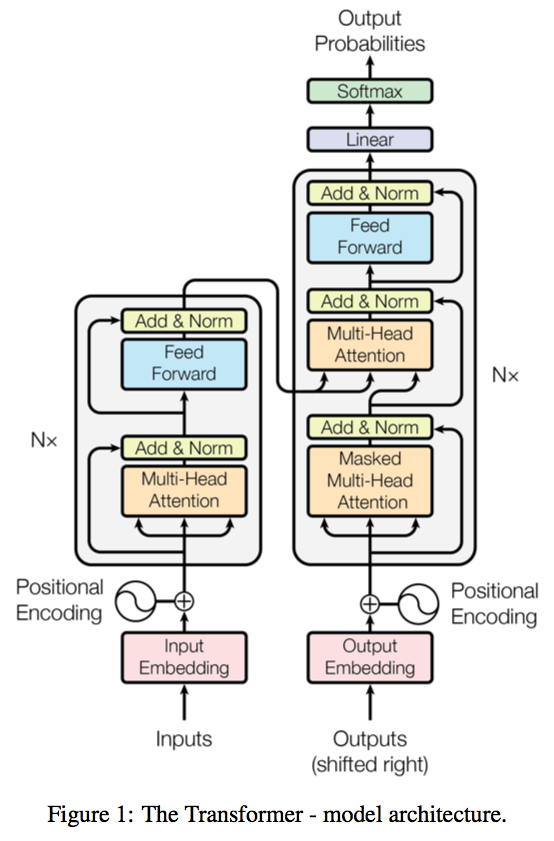
\includegraphics[width=0.35\linewidth,keepaspectratio]{transformer}
	\end{center}		

{\tiny (Ref: ``Attention is all you need''. 2017.  Aswani, Shazeer, Parmar, Uszkoreit,  Jones, Gomez, Kaiser, Polosukhin  https://arxiv.org/pdf/1706.03762.pdf}


			
\end{frame}

%%%%%%%%%%%%%%%%%%%%%%%%%%%%%%%%%%%%%%%%%%%%%%%%%%%%%%%%%%%
\begin{frame}[fragile]\frametitle{A High-Level Look}

Lets start with a very high-level view \ldots and then Zoom in each sub-blocks.

Here is the Transformer block and its i/o.

\begin{center}
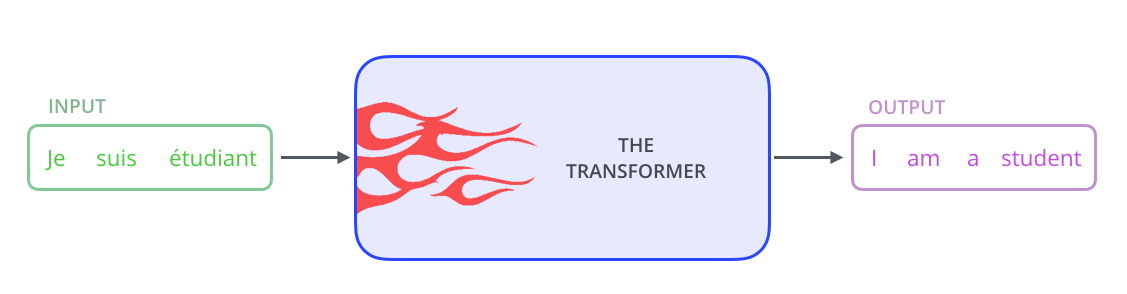
\includegraphics[width=0.8\linewidth,keepaspectratio]{transformer_jay}

{\tiny (Ref: ``The Illustrated Transformer'' - Jay Alammar)}
\end{center}		

\begin{itemize}
\item Main architecture: encoder-decoder ie sequence to sequence
\item Task: machine translation with parallel corpus (encoder-decoder)
\item Sub-tasks: Word Embedding (Encoder), Predict each translated word (Decoder)
\item can be done by RNNs, LSTMs, etc. But they had issues.
\item Here we bring parallelization.
\item Challenges? Different input-output sizes, different attention correspondence, word order matters, semantic preservation, compute cost, storage cost, etc.
\end{itemize}

			
\end{frame}

%%%%%%%%%%%%%%%%%%%%%%%%%%%%%%%%%%%%%%%%%%%%%%%%%%%%%%%%%%%
\begin{frame}[fragile]\frametitle{One level down}

Within Transformer block we have

\begin{center}
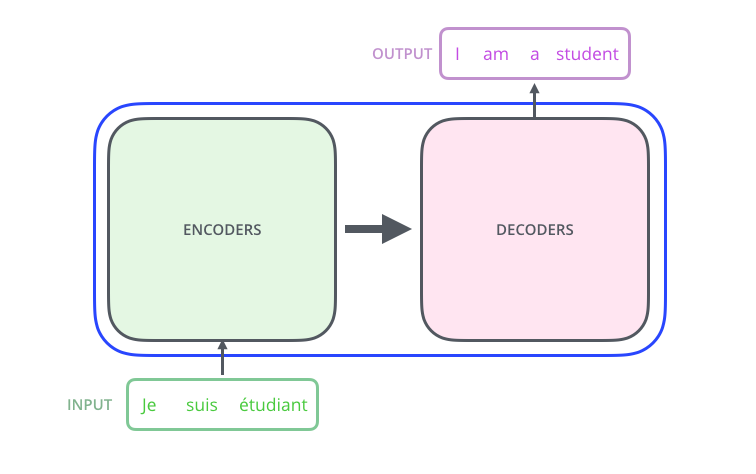
\includegraphics[width=0.6\linewidth,keepaspectratio]{transformer_encoders_decoders_jay}

{\tiny (Ref: ``The Illustrated Transformer'' - Jay Alammar)}
\end{center}		

Inference time flow: 
\begin{itemize}
\item Encoder takes input
\item Does some processing, creates a `latent` representation, sends it to decoder
\item Decoder processes this input to generate the output
\end{itemize}

What would be ML training flow?
			
\end{frame}

%%%%%%%%%%%%%%%%%%%%%%%%%%%%%%%%%%%%%%%%%%%%%%%%%%%%%%%%%%%
\begin{frame}[fragile]\frametitle{One level down}

Each sub-block ie Encoder-Decoder blocks are actually stacks of encoders decoders.

\begin{center}
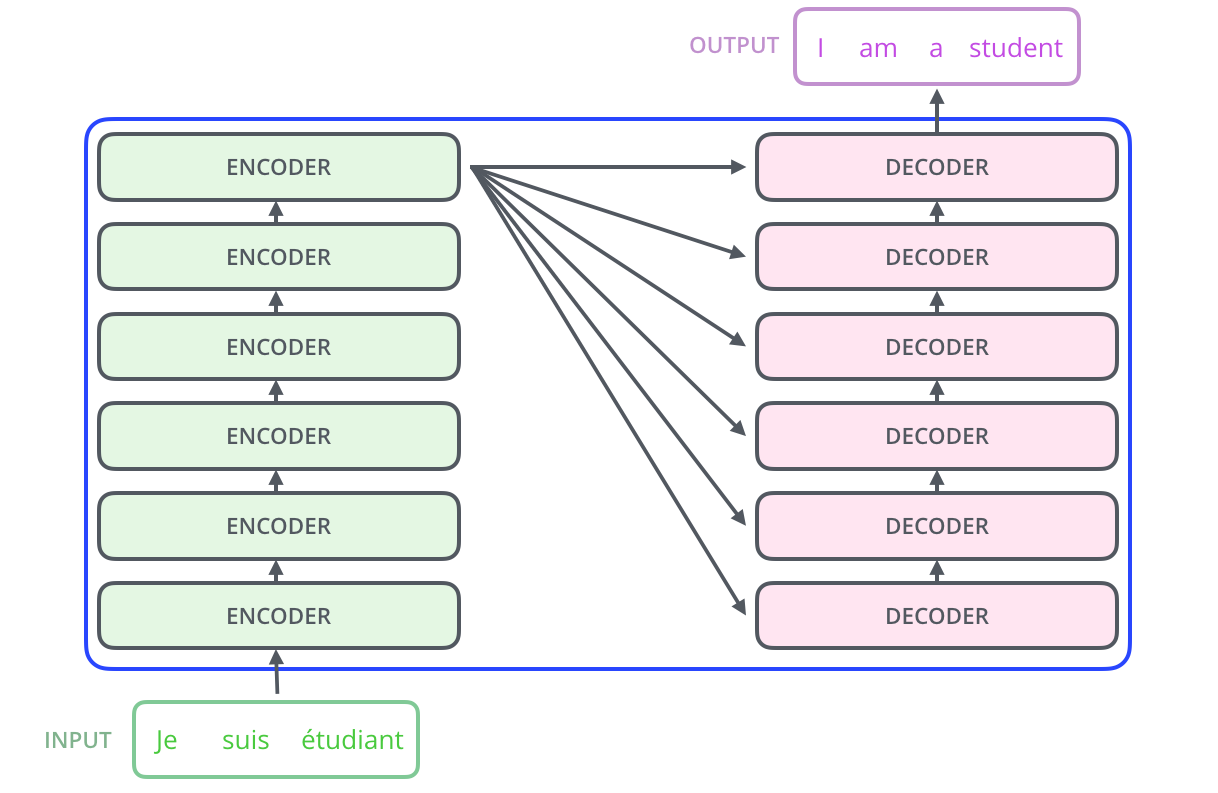
\includegraphics[width=0.6\linewidth,keepaspectratio]{transformer_encoder_decoder_stack_jay}

{\tiny (Ref: ``The Illustrated Transformer'' - Jay Alammar)}
\end{center}		

 
\begin{itemize}
\item Encoder has 6 blocks, so does Decoder. 
\item Why 6? Why not 7? They found it to be good. Like Hyper-parameter.
\end{itemize}

How many blocks GPT 3.5 has?
			
\end{frame}

%%%%%%%%%%%%%%%%%%%%%%%%%%%%%%%%%%%%%%%%%%%%%%%%%%%%%%%%%%%
\begin{frame}[fragile]\frametitle{One level down in Encoder Cell}

Each Encoder sub-block is actually stack of \ldots

\begin{columns}
    \begin{column}[T]{0.5\linewidth}
		\begin{center}
		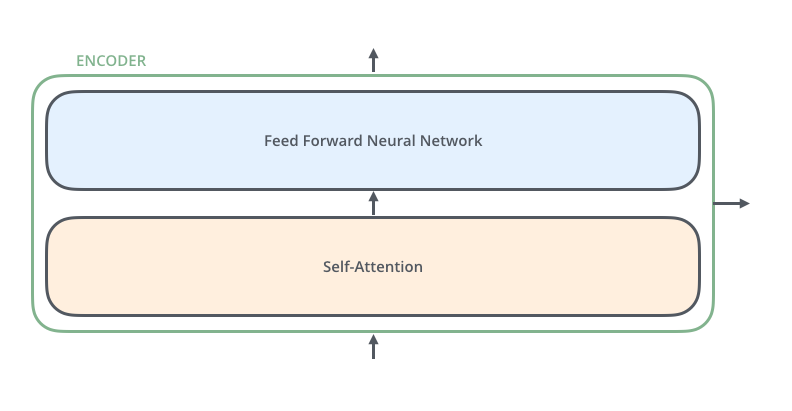
\includegraphics[width=\linewidth,keepaspectratio]{transformer_encoder_jay}
		
		{\tiny (Ref: ``The Illustrated Transformer'' - Jay Alammar)}
		\end{center}		
	\end{column}
	\begin{column}[T]{0.5\linewidth}
		\begin{itemize}
		\item Self Attention:  a layer that helps the encoder look at other words in the input sentence as it encodes a specific word.
		\item Feed Forward: The outputs of the self-attention layer are fed to a feed-forward neural network. The exact same feed-forward network is independently applied to each position.
		\end{itemize}
	\end{column}
\end{columns}
Input Embedding? Positional Embedding? Residual connections? batch normalization?
			
\end{frame}


%%%%%%%%%%%%%%%%%%%%%%%%%%%%%%%%%%%%%%%%%%%%%%%%%%%%%%%%%%%
\begin{frame}[fragile]\frametitle{Similarly on Decoder side}

Each Decoder sub-block is actually stack of \ldots


		\begin{center}
		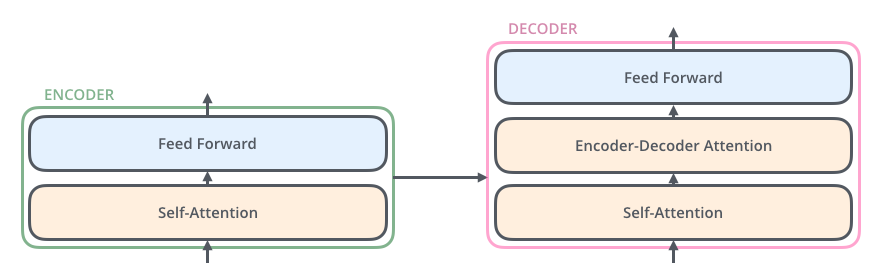
\includegraphics[width=\linewidth,keepaspectratio]{transformer_decoder_jay}
		
		{\tiny (Ref: ``The Illustrated Transformer'' - Jay Alammar)}

		\end{center}		
		

		\begin{itemize}
		\item The decoder also has both those layers (Self but Masked Attention and Feed Forward), but between them is an (cross) attention layer that helps the decoder focus on relevant parts of the input sentence
		\end{itemize}

		
\end{frame}

%%%%%%%%%%%%%%%%%%%%%%%%%%%%%%%%%%%%%%%%%%%%%%%%%%%%%%%%%%%
\begin{frame}[fragile]\frametitle{Transformer Encoder}

Actual architecture in the research paper.

\begin{columns}
    \begin{column}[T]{0.4\linewidth}
			\begin{center}
			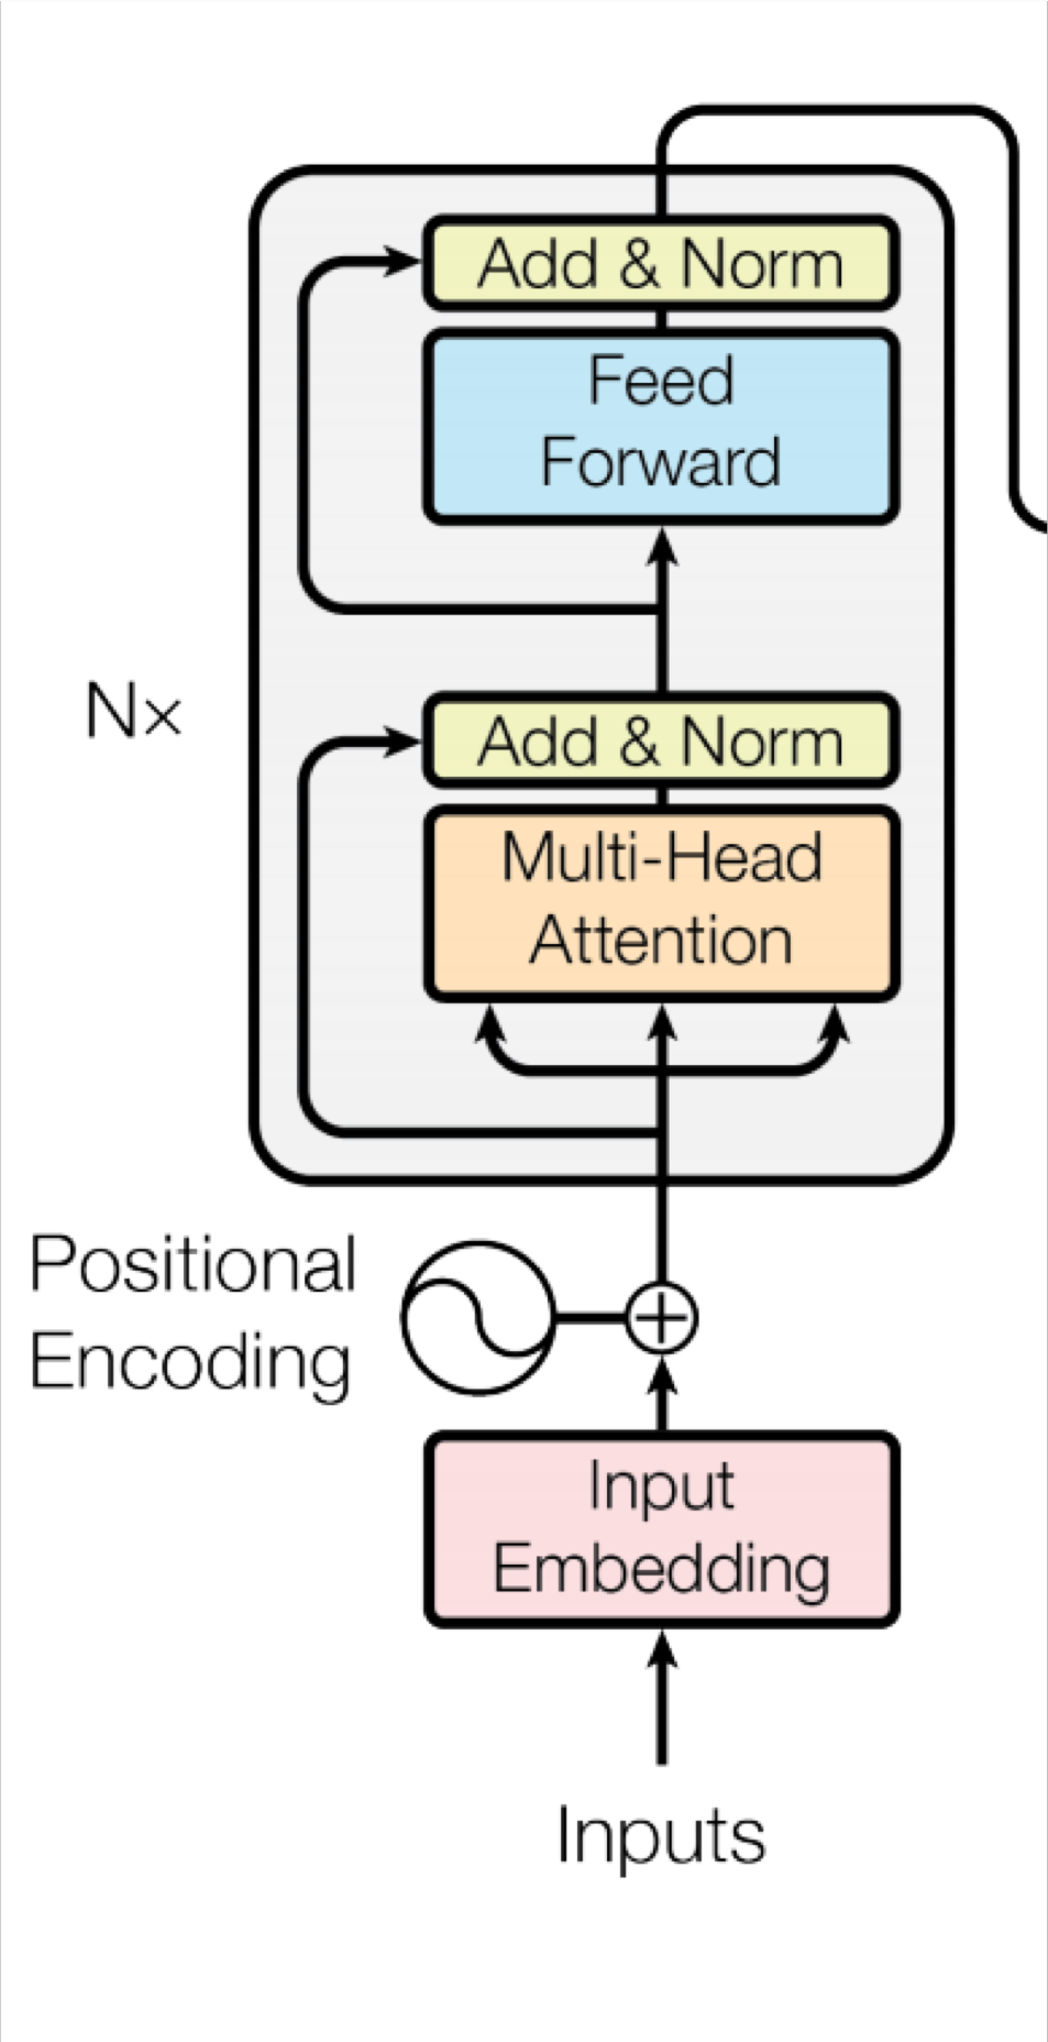
\includegraphics[width=0.6\linewidth,keepaspectratio]{bert70}
			\end{center}		
		\end{column}
    \begin{column}[T]{0.6\linewidth}
      \begin{itemize}
			\item For encoder block, initial input, tokenization, embedding, positional encoding, happens at the start, then the first Encoder cell starts.
			\item In each cell, we have multi-head self attention, residual connections, batch normalization and then feed forward then again residual + batch normalization.
			\item Output of this cell is passed to the next encoder cell.
			\item Output of the last encoder cell in the encoder block is passed to the Decoder block.
			\end{itemize}
    \end{column}
  \end{columns}
		
     \begin{itemize}
			\item Mind well, that each word here gets processed parallelly, unlike RNN or LSTM.
			\item Cells are repeated 6 times (in vertical stack)
			\end{itemize}		
\end{frame}

%%%%%%%%%%%%%%%%%%%%%%%%%%%%%%%%%%%%%%%%%%%%%%%%%%%%%%%%%%%
\begin{frame}[fragile]\frametitle{Transformer Decoder}


			\begin{center}
			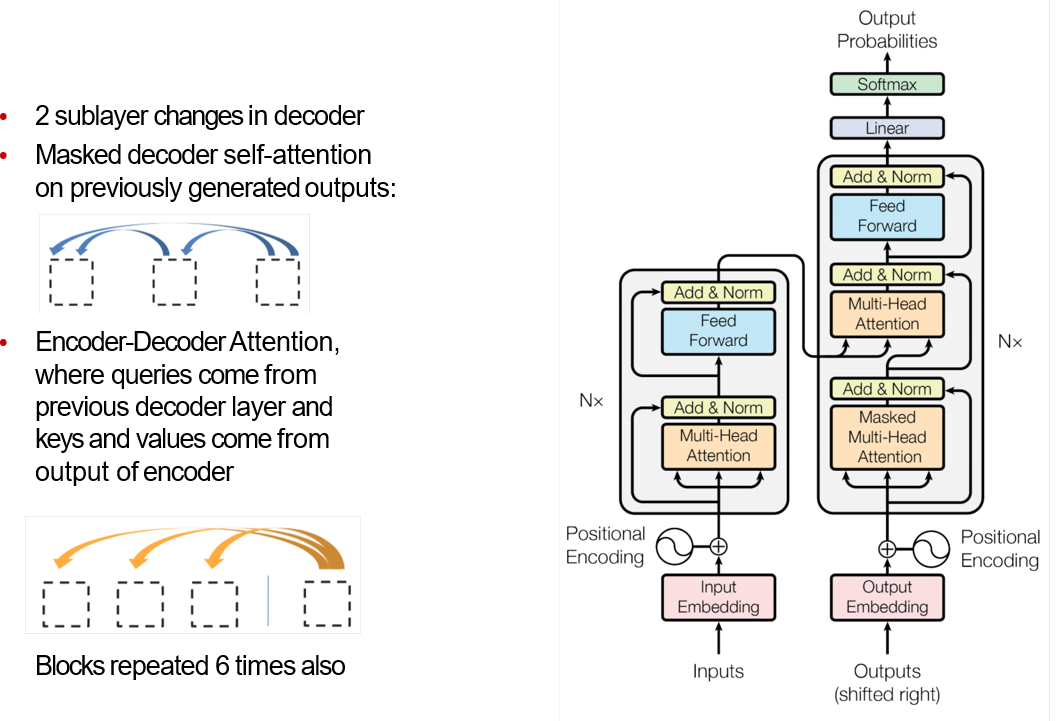
\includegraphics[width=\linewidth,keepaspectratio]{bert71}
			\end{center}		

			
\end{frame}

%%%%%%%%%%%%%%%%%%%%%%%%%%%%%%%%%%%%%%%%%%%%%%%%%%%%%%%%%%%
\begin{frame}[fragile]\frametitle{Transformer Encoder-Decoder}

			\begin{center}
			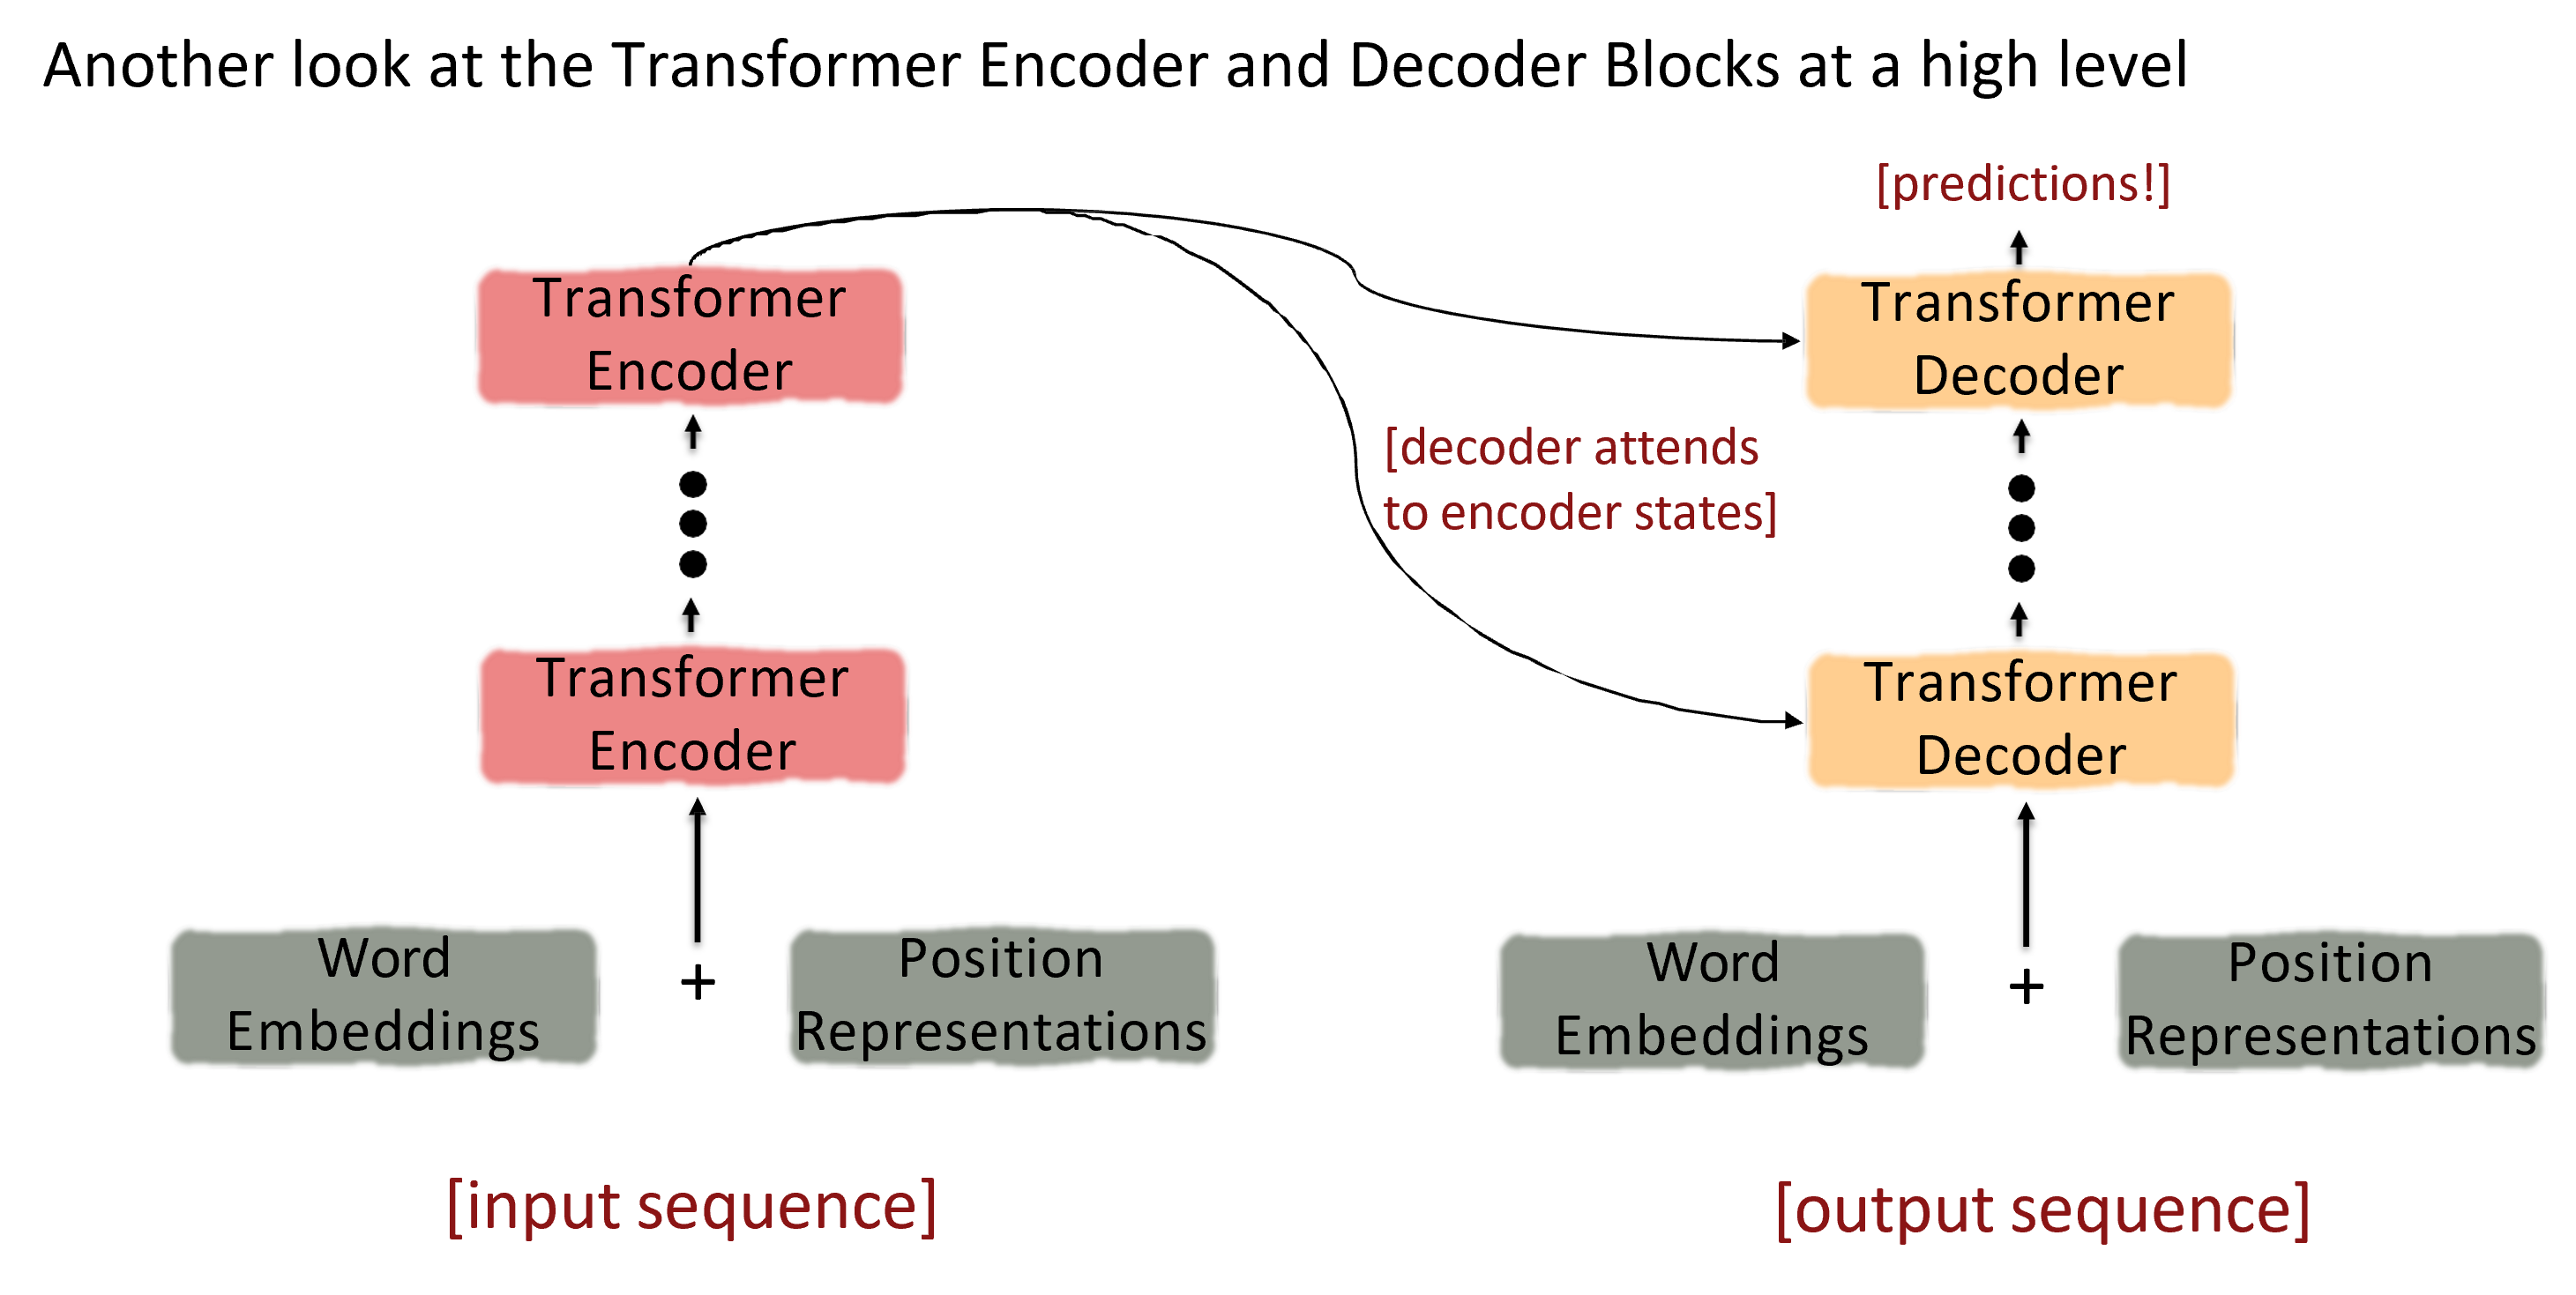
\includegraphics[width=\linewidth,keepaspectratio]{bert72}
			\end{center}		

			
\end{frame}

%%%%%%%%%%%%%%%%%%%%%%%%%%%%%%%%%%%%%%%%%%%%%%%%%%%%%%%%%%%
\begin{frame}[fragile]\frametitle{Transformer Encoder-Decoder}
Next, let’s look at the Transformer Encoder and Decoder Blocks in action


      \begin{itemize}
			\item Imagine Machine Translation: French to English
			\item What would be ML training flow?
			\item What would be ML inference flow?
			\item Can we use input or output text as is, ie in string format?
			\item Whats the NLP way of making text available for ML or DL algorithms?
	\end{itemize}
			
\end{frame}

%%%%%%%%%%%%%%%%%%%%%%%%%%%%%%%%%%%%%%%%%%%%%%%%%%%%%%%%%%%%%%%%%%%%%%%%%%%%%%%%%%
\begin{frame}[fragile]\frametitle{}
\begin{center}
{\Large Block: Input Embedding}
\end{center}
\end{frame}

%%%%%%%%%%%%%%%%%%%%%%%%%%%%%%%%%%%%%%%%%%%%%%%%%%%%%%%%%%%
\begin{frame}[fragile]\frametitle{Convert Sentence to Tokens}


\begin{itemize}
\item Each word can be one or more tokens
\item Subword tokenization, prefixes, suffixes, etc
\item Highly Language dependent, imagine Sanskrit tokenization
\item Each model will have its corresponding tokenizer, thusr forming vocabulary array, word-to-id
\item ``I love cats''  could be tokenised to $[816, 8129, 312]$
\end{itemize}

For now, we can use `Toekn` and `Word` synonymously.

\end{frame}

%%%%%%%%%%%%%%%%%%%%%%%%%%%%%%%%%%%%%%%%%%%%%%%%%%%%%%%%%%%
\begin{frame}[fragile]\frametitle{Convert Tokens to Vectors}


\begin{center}
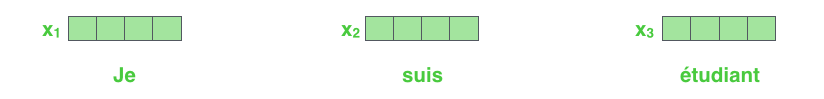
\includegraphics[width=\linewidth,keepaspectratio]{embeddings_jay}


{\tiny (Ref: ``The Illustrated Transformer'' - Jay Alammar)}
\end{center}		


\begin{itemize}
\item Either by Frequency based ie one-hot or tf-idf or Neural way ie Word2Vec (in paper)
\item Or put embedding layer (like in TensorFlow or Keras NLP, which also gets trained)
\item Size: 512, a hyper-parameter we can set – basically it would be the length of the longest sentence in our training dataset.
\item After embedding the words in our input sequence, each of them flows through each of the two layers of the encoder.
\end{itemize}

% \begin{lstlisting}
% I: [0.34, -0.21, 1.21]
% love: [-1.36, 0.98, 0.23]
% cats: [0.54, 0.68, 0.49]
% \end{lstlisting}
\end{frame}

%%%%%%%%%%%%%%%%%%%%%%%%%%%%%%%%%%%%%%%%%%%%%%%%%%%%%%%%%%%
\begin{frame}[fragile]\frametitle{Flow of Vectors in Encoder Cell}


\begin{columns}
    \begin{column}[T]{0.5\linewidth}
\begin{center}
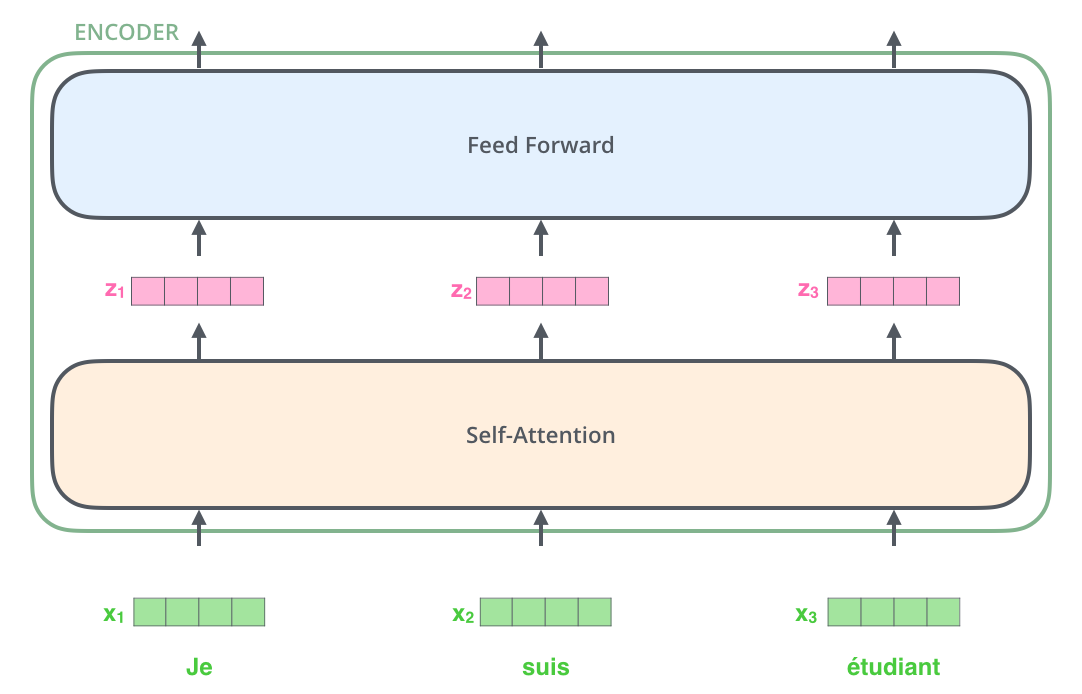
\includegraphics[width=\linewidth,keepaspectratio]{encoder_with_tensors_jay}


{\tiny (Ref: ``The Illustrated Transformer'' - Jay Alammar)}
\end{center}		

		\end{column}
    \begin{column}[T]{0.5\linewidth}
\begin{itemize}
\item Key property : the word in each position flows through its own path in the encoder. 
\item Calculations in the self-attention layer do need other words. 
\item But later, in the feed-forward layer does not have those dependencies, \item thus the various paths can be executed in parallel while flowing through the feed-forward layer.
\end{itemize}
    \end{column}
  \end{columns}
\end{frame}

%%%%%%%%%%%%%%%%%%%%%%%%%%%%%%%%%%%%%%%%%%%%%%%%%%%%%%%%%%%
\begin{frame}[fragile]\frametitle{Flow of Vectors in Encoder Block}


\begin{center}
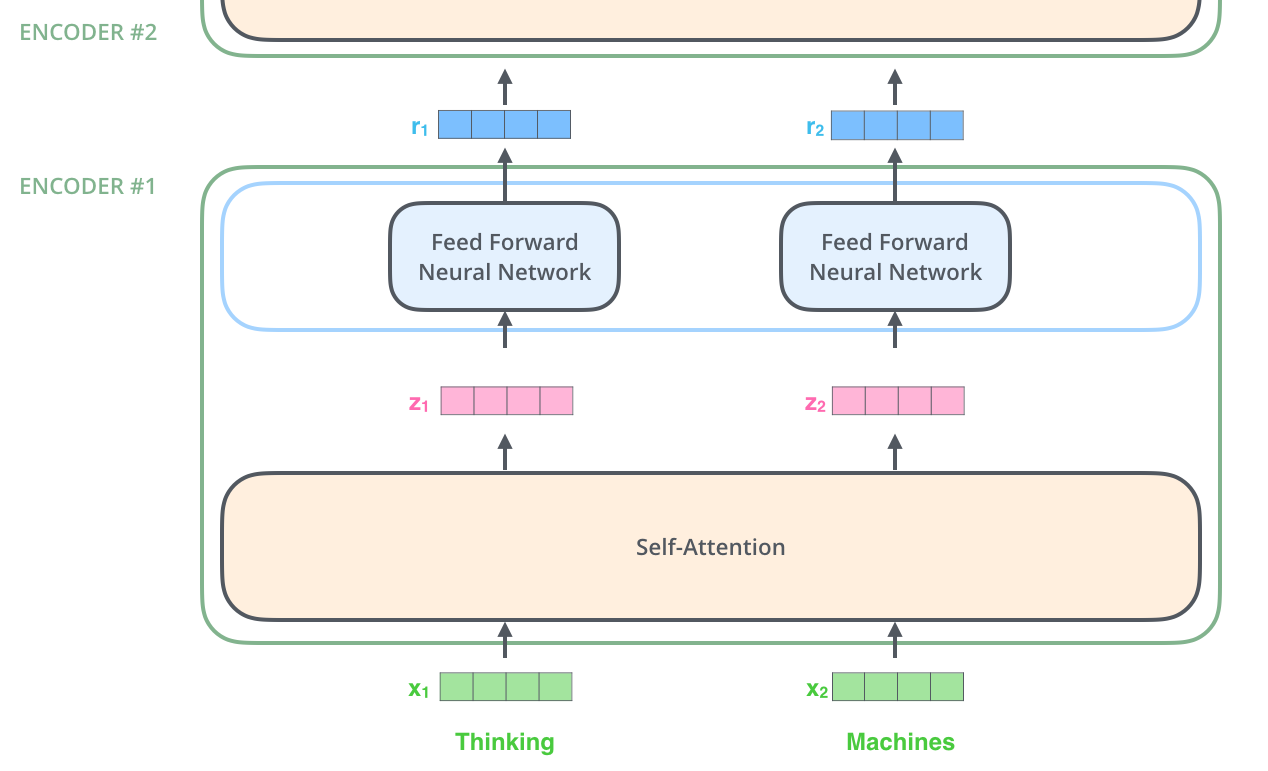
\includegraphics[width=0.6\linewidth,keepaspectratio]{encoder_with_tensors_block_jay}


{\tiny (Ref: ``The Illustrated Transformer'' - Jay Alammar)}
\end{center}		


\begin{itemize}
\item The word at each position passes through a self-attention process. 
\item Then, they each pass through a feed-forward neural network -- the exact same network with each vector flowing through it separately.
\item Meaning ALL weights in these cells, block are same for ALL words going through in each epoch, of course they get adjusted during back propagation.
\end{itemize}

\end{frame}


%%%%%%%%%%%%%%%%%%%%%%%%%%%%%%%%%%%%%%%%%%%%%%%%%%%%%%%%%%%%%%%%%%%%%%%%%%%%%%%%%%
\begin{frame}[fragile]\frametitle{}
\begin{center}
{\Large Block: Positional Encoding}
\end{center}
\end{frame}

%%%%%%%%%%%%%%%%%%%%%%%%%%%%%%%%%%%%%%%%%%%%%%%%%%%%%%%%%%%
\begin{frame}[fragile]\frametitle{Why?}


\begin{itemize}
\item In languages like English (unlike Sanskrit) word order matters, meaning 'Suresh ate chicken' and 'chicken ate Suresh' are two different things.
\item As input is all word vectors together, parallel, (unlike RNN or LSTM where they are sequential ie one after another, there the order is preserved), the sense of position is lost.
\item Need to add that information by unique position value/signature.
\item There are many reasons why a single number, such as the index value, is not used to represent an item’s position in transformer models. 
\item For long sequences, the indices can grow large in magnitude. 
\item If you normalize the index value to lie between 0 and 1, it can create problems for variable length sequences as they would be normalized differently.
\item A cool mechanism (similar to Fourier Transform) was employed.
\item This mechanism is such that uniqueness/signature of a position is achieved and also the distance requirement is fulfilled, meaning neighboring words have less distance and vice versa.
\end{itemize}

\end{frame}

%%%%%%%%%%%%%%%%%%%%%%%%%%%%%%%%%%%%%%%%%%%%%%%%%%%%%%%%%%%
\begin{frame}[fragile]\frametitle{What?}

{\bf Note}: Confirm that uniqueness/signature of a position is achieved and also the distance requirement is fulfilled, meaning neighboring words have less distance and vice versa.



\begin{lstlisting}
Position 1: [0.1, 0.2, 0.3]
Position 2: [0.4, 0.5, 0.6]
Position 3: [0.7, 0.8, 0.9]

Combine Embeddings and Positional Encodings

I (position 1) = [0.34 + 0.1, -0.21 + 0.2, 1.21 + 0.3] = [0.44, -0.01, 1.51]
love (position 2) = [-1.36 + 0.4, 0.98 + 0.5, 0.23 + 0.6] = [-0.96, 1.48, 0.83]
cats (position 3) = [0.54 + 0.7, 0.68 + 0.8, 0.49 + 0.9] = [1.24, 1.48, 1.39]
\end{lstlisting}


\end{frame}



%%%%%%%%%%%%%%%%%%%%%%%%%%%%%%%%%%%%%%%%%%%%%%%%%%%%%%%%%%%
\begin{frame}[fragile]\frametitle{Representing The Order of The Sequence Using Positional Encoding}


\begin{columns}
    \begin{column}[T]{0.5\linewidth}
\begin{center}
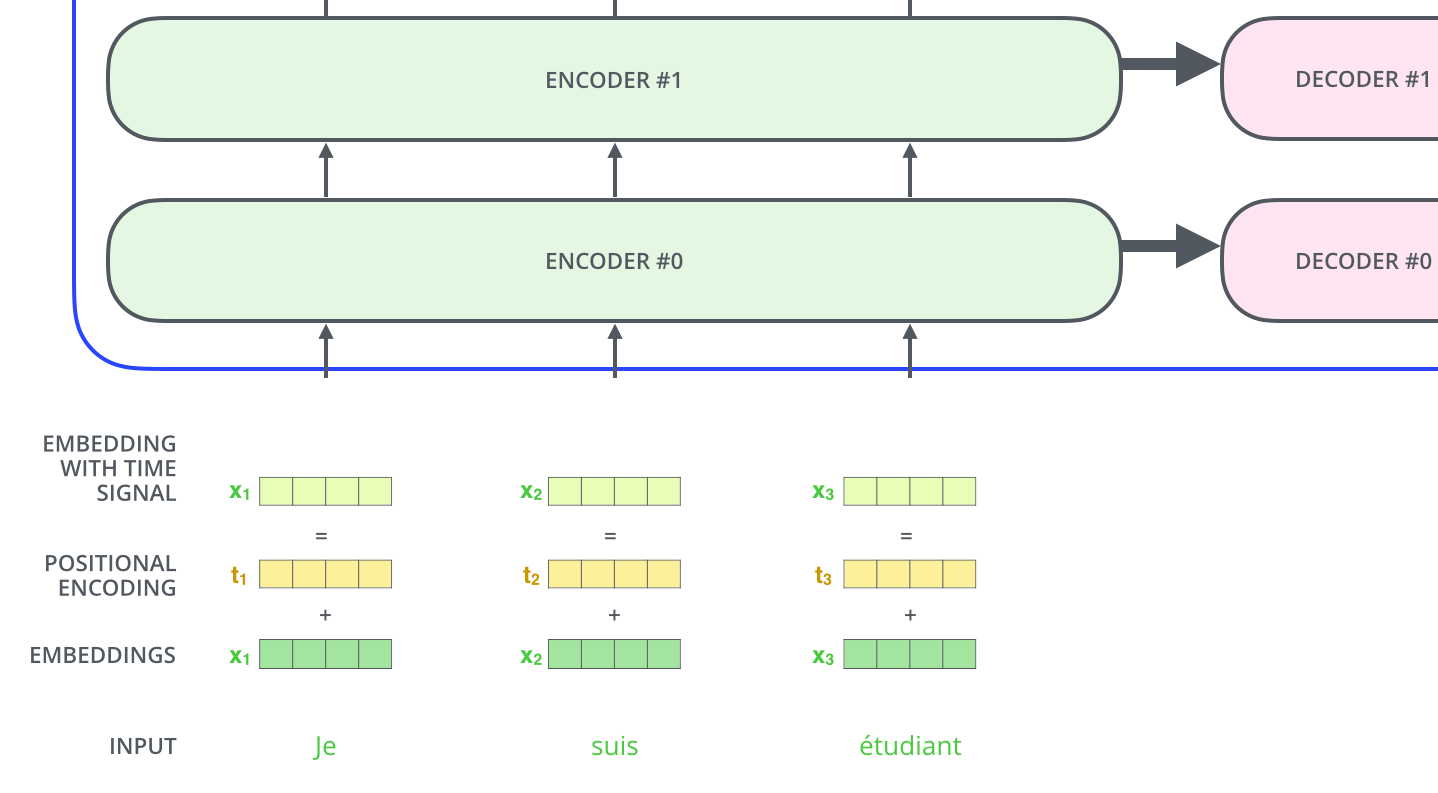
\includegraphics[width=\linewidth,keepaspectratio]{transformer_positional_encoding_vectors_jay}

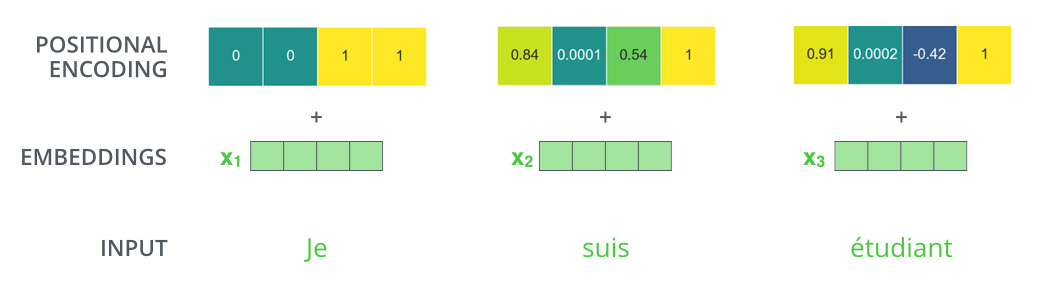
\includegraphics[width=\linewidth,keepaspectratio]{transformer_positional_encoding_example_jay}


{\tiny (Ref: ``The Illustrated Transformer'' - Jay Alammar)}
\end{center}		

		\end{column}
    \begin{column}[T]{0.5\linewidth}

\begin{itemize}
\item Special pattern based vectors encode position or the distance between different words in the sequence. 
\item Using sine waves of different phase lags and amplitude to create unique set of basis functions, equal to number of words in the sentence.
\item They are added to input word embedding.
\end{itemize}
    \end{column}
  \end{columns}
\end{frame}



%%%%%%%%%%%%%%%%%%%%%%%%%%%%%%%%%%%%%%%%%%%%%%%%%%%%%%%%%%%
\begin{frame}[fragile]\frametitle{Positional Patterns}

\begin{itemize}
\item The Position Encoding is computed independently of the input sequence. 
\item These are fixed values that depend only on the max length of the sequence. 
\end{itemize}

$PE_{(pos,2i)} = sin(pos/n^{2i/d_{model}})$


$PE_{(pos,2i+1)} = cos(pos/n^{2i/d_{model}})$

\begin{itemize}
\item $pos$ is the position of the word in the sequence
\item $n$ is User-defined scalar, set to 10,000 by the authors of Attention Is All You Need.
\item $d_{model}$ is the length of the encoding vector (same as the embedding vector) and
\item $i$ is the index value into this vector.Used for mapping to column indices $0 \leq i < d/2$ , with a single value of $i$
 maps to both sine and cosine functions
\end{itemize}

{\tiny (Ref: Transformers Explained Visually - How it works, step-by-step - Ketan Doshi)}

\end{frame}

%%%%%%%%%%%%%%%%%%%%%%%%%%%%%%%%%%%%%%%%%%%%%%%%%%%%%%%%%%%
\begin{frame}[fragile]\frametitle{What Formula Means?}

\begin{itemize}
\item $pos$ is on x axis and encoded value is on y axis.
\item If we had used just one wave, two words, say `Why' and `are` would have got same y value, so no use!!
\item Have more waves, with phase lag and different frequencies (due to $2i/d_{model}$ part of the equation
\item So, for these words, their y values for diff waves would be different, making them unique.
\end{itemize}


\begin{center}
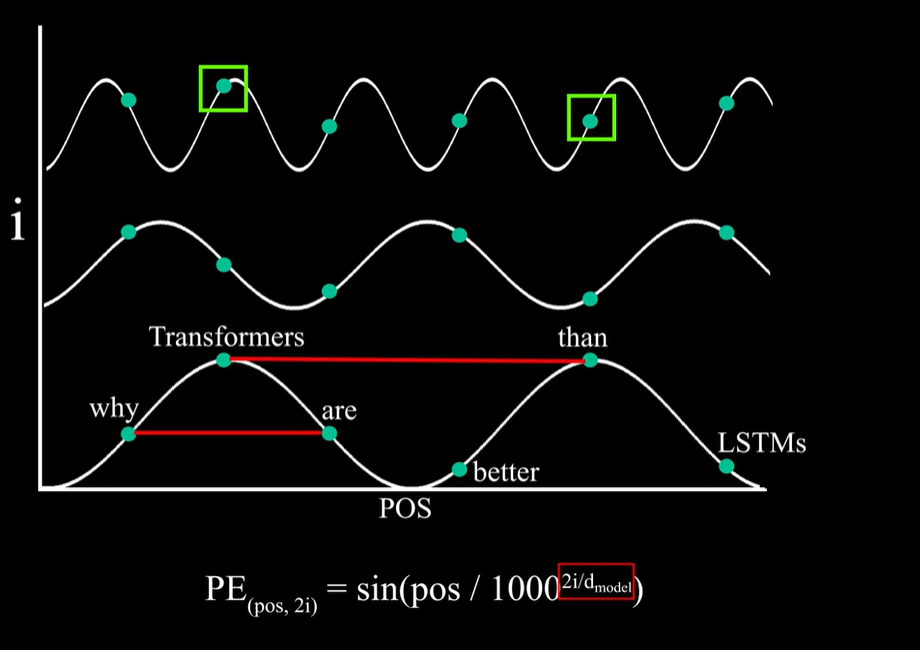
\includegraphics[width=0.5\linewidth,keepaspectratio]{positional_encoding_5}


{\tiny (Ref: ``Attention is all you need || Transformers Explained || Quick Explained'' - Developers Hutt)}
\end{center}		

\end{frame}

%%%%%%%%%%%%%%%%%%%%%%%%%%%%%%%%%%%%%%%%%%%%%%%%%%%%%%%%%%%
\begin{frame}[fragile]\frametitle{Mechanism}


\begin{center}
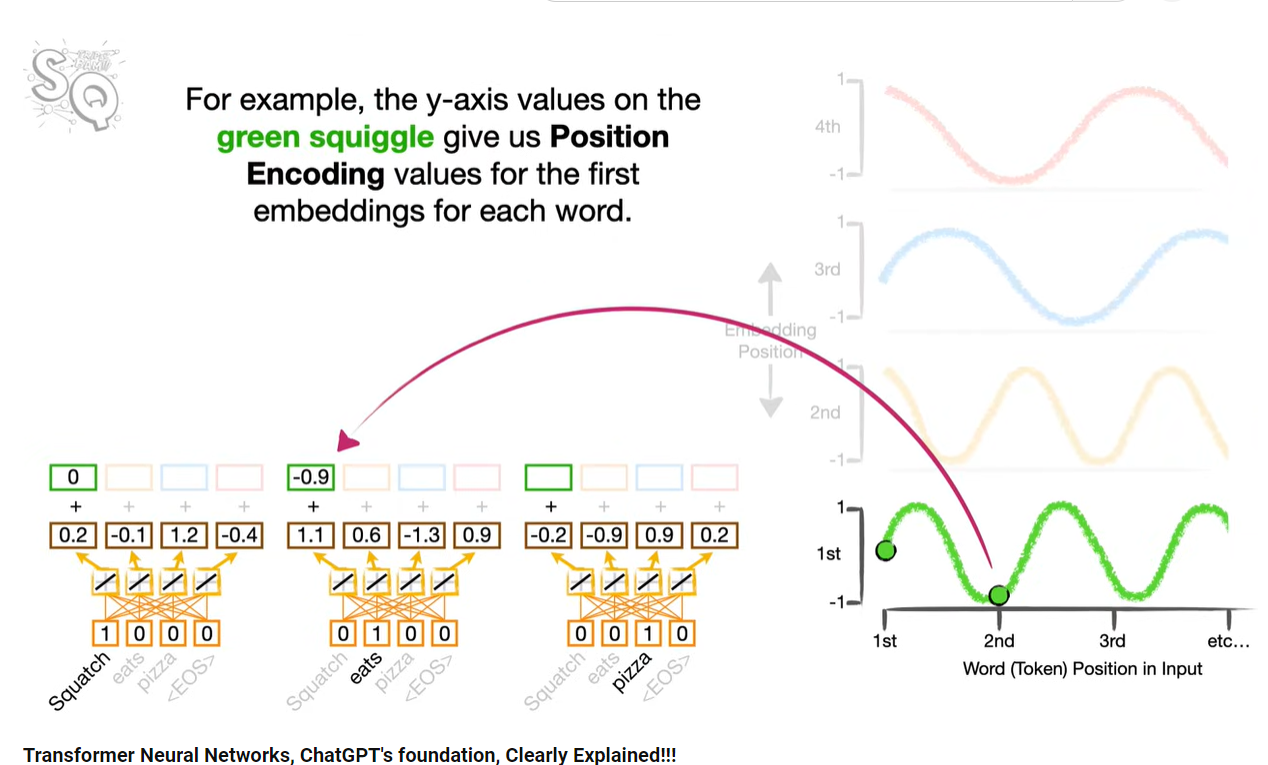
\includegraphics[width=\linewidth,keepaspectratio]{positional_encoding_3}


{\tiny (Ref: StatQuest with Josh Starmer)}
\end{center}		

\end{frame}

%%%%%%%%%%%%%%%%%%%%%%%%%%%%%%%%%%%%%%%%%%%%%%%%%%%%%%%%%%%
\begin{frame}[fragile]\frametitle{Mechanism}


\begin{center}
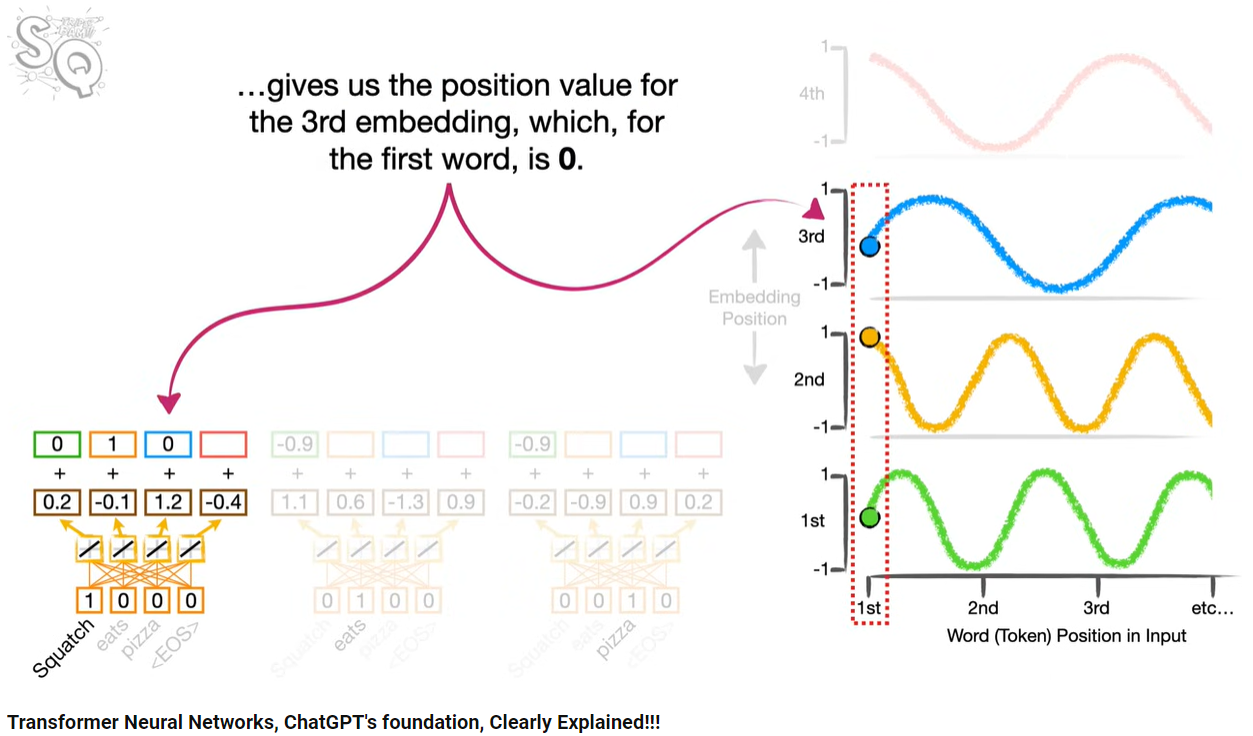
\includegraphics[width=\linewidth,keepaspectratio]{positional_encoding_4}


{\tiny (Ref: StatQuest with Josh Starmer)}
\end{center}		

\end{frame}

%%%%%%%%%%%%%%%%%%%%%%%%%%%%%%%%%%%%%%%%%%%%%%%%%%%%%%%%%%%
\begin{frame}[fragile]\frametitle{Mechanism}

Each position/index is mapped to a vector

\begin{center}
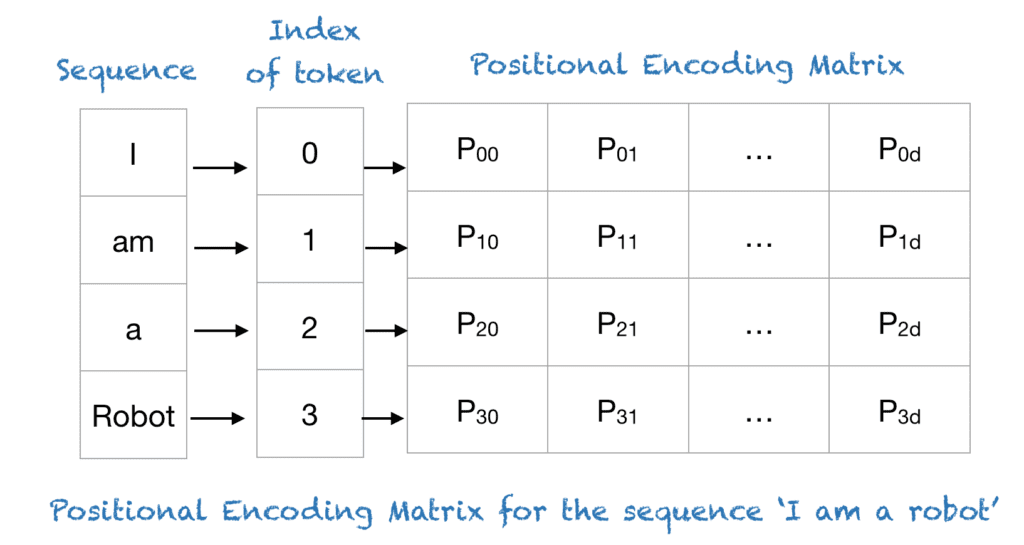
\includegraphics[width=\linewidth,keepaspectratio]{positional_encoding_1}


{\tiny (Ref: ``A Gentle Introduction to Positional Encoding in Transformer Models, Part 1'' - Mehreen Saeed)}
\end{center}		

\end{frame}


%%%%%%%%%%%%%%%%%%%%%%%%%%%%%%%%%%%%%%%%%%%%%%%%%%%%%%%%%%%
\begin{frame}[fragile]\frametitle{Mechanism}

Each position/index is mapped to a vector

\begin{center}
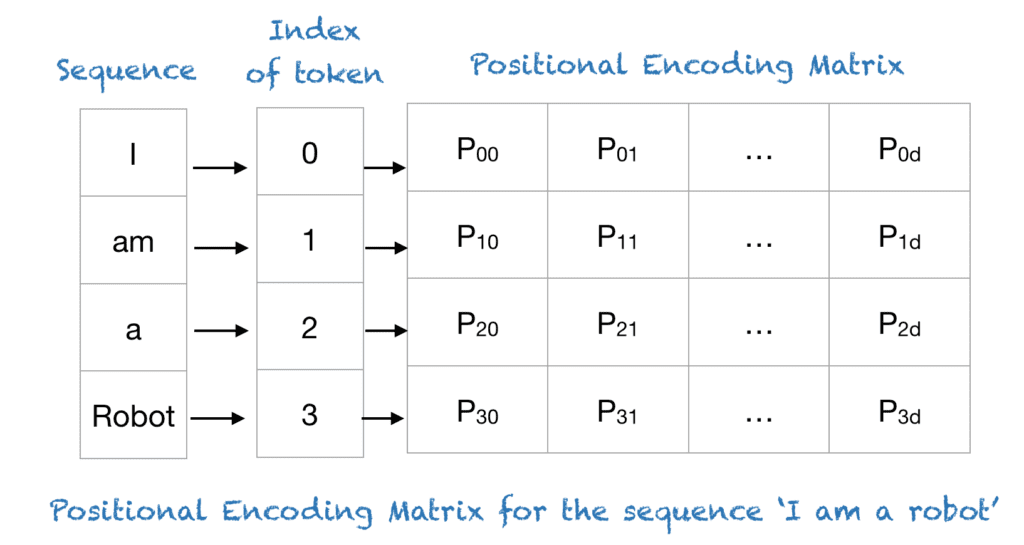
\includegraphics[width=\linewidth,keepaspectratio]{positional_encoding_1}


{\tiny (Ref: ``A Gentle Introduction to Positional Encoding in Transformer Models, Part 1'' - Mehreen Saeed)}
\end{center}		

\end{frame}

%%%%%%%%%%%%%%%%%%%%%%%%%%%%%%%%%%%%%%%%%%%%%%%%%%%%%%%%%%%
\begin{frame}[fragile]\frametitle{Example}

Each position/index is mapped to a vector

\begin{center}
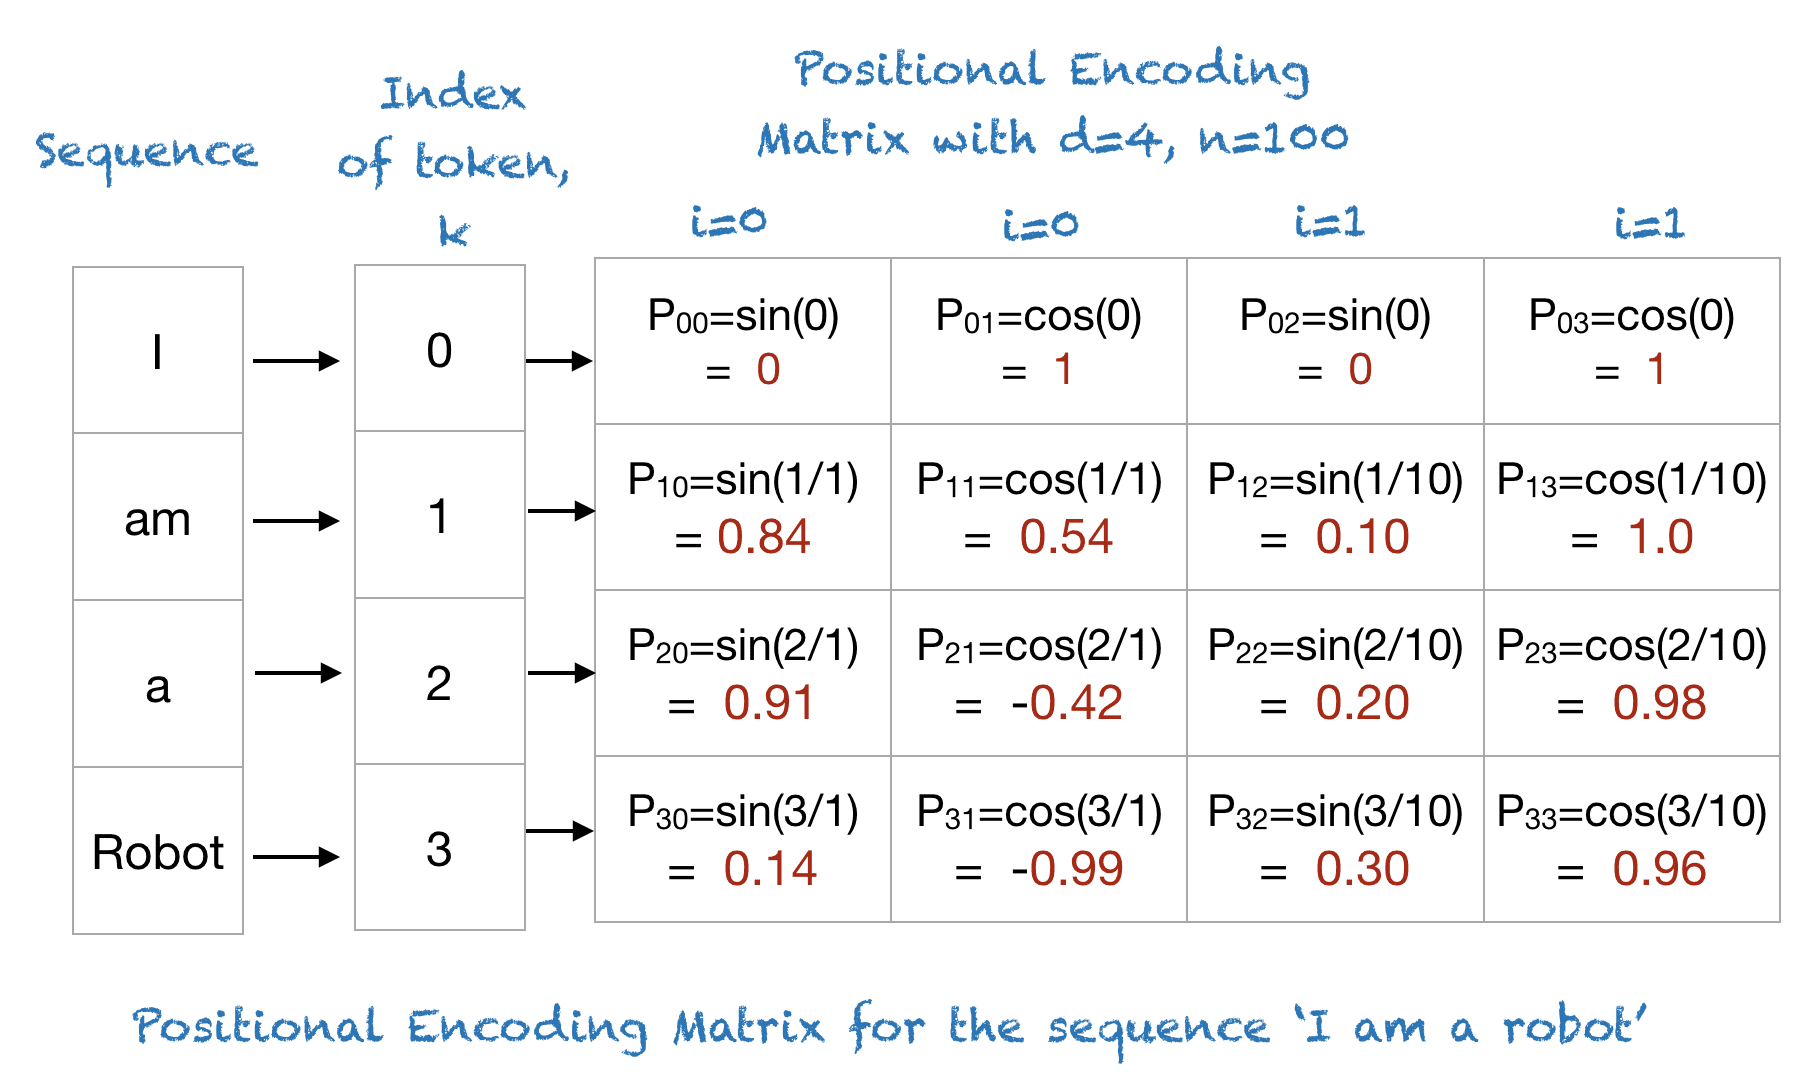
\includegraphics[width=\linewidth,keepaspectratio]{positional_encoding_2}


{\tiny (Ref: ``A Gentle Introduction to Positional Encoding in Transformer Models, Part 1'' - Mehreen Saeed)}
\end{center}		

\end{frame}


%%%%%%%%%%%%%%%%%%%%%%%%%%%%%%%%%%%%%%%%%%%%%%%%%%%%%%%%%%%%%%%%%%%%%%%%%%%%%%%%%%
\begin{frame}[fragile]\frametitle{}
\begin{center}
{\Large Self Attention}
\end{center}
\end{frame}

%%%%%%%%%%%%%%%%%%%%%%%%%%%%%%%%%%%%%%%%%%%%%%%%%%%%%%%%%%%
\begin{frame}[fragile]\frametitle{Self-Attention at a High Level}

\begin{columns}
    \begin{column}[T]{0.5\linewidth}
\begin{center}
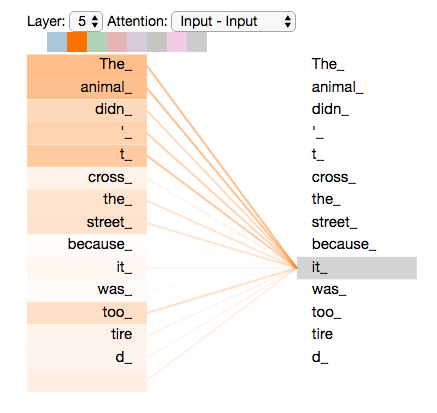
\includegraphics[width=\linewidth,keepaspectratio]{transformer_self-attention_visualization_jay}


{\tiny (Ref: ``The Illustrated Transformer'' - Jay Alammar)}
\end{center}		

		\end{column}
    \begin{column}[T]{0.5\linewidth}

\begin{itemize}
\item ``The animal didn't cross the street because it was too tired'', what ``it'' refers to?
\item  the street or to the animal?
\item For “it”, self-attention mechanism (some how, or should) allows it to associate “it” with “animal”.
\item ie for each word (each position in the input sequence), self attention allows it to look at other positions in the input sequence for clues that can help lead to a better encoding for this word.
\item Lets see how that can be achieved.
\end{itemize}
    \end{column}
  \end{columns}
\end{frame}

%%%%%%%%%%%%%%%%%%%%%%%%%%%%%%%%%%%%%%%%%%%%%%%%%%%%%%%%%%%
\begin{frame}[fragile]\frametitle{Self-Attention in Principle}


\begin{itemize}
\item Slight digression: lets say you have database of key($k$)-value($v$) pairs, then you have a query ($q$), which needs to go and search in the database and get corresponding or closest value.
\item So, $q$ is matched (similarity) with all $k$s, whichever matches most, its $v$ is returned.
% \item Same mechanism is used to create self-attention score.
% \item For each word-vector in the sentence ($q$), we find similarity with $k$ vectors or all the words, which ever matches most, its $v$ vector is returned.
\item The Query word can be interpreted as the word for which we are calculating Attention. The Key and Value word is the word to which we are paying attention ie. how relevant is that word to the Query word.
\item For example, for the sentence, “The ball is blue”, the row for the word “blue” will contain the attention scores for “blue” with every other word. Here, “blue” is the Query word, and the other words are the “Key/Value”.
\end{itemize}

\end{frame}

%%%%%%%%%%%%%%%%%%%%%%%%%%%%%%%%%%%%%%%%%%%%%%%%%%%%%%%%%%%
\begin{frame}[fragile]\frametitle{Self-Attention in Principle}


$W_q$, $W_k$, and $W_v$ are learned during training and are shared between all of the embedding vectors.

\begin{lstlisting}
I = `[0.44, -0.01, 1.51]`
love = `[-0.96, 1.48, 0.83]`
cats  = `[1.24, 1.48, 1.39]`

``I'' = 
`[0.44, -0.01, 1.51] * W_q = Q_1` 
`[0.44, -0.01, 1.51] * W_k = K_1`
`[0.44, -0.01, 1.51] * W_v = V_1`

``love'' = 
`[-0.96, 1.48, 0.83] * W_q = Q_2`  
`[-0.96, 1.48, 0.83] * W_k = K_2`  
`[-0.96, 1.48, 0.83] * W_v = V_2`  

``cats'' = 
`[1.24, 1.48, 1.39] * W_q = Q_3`  
`[1.24, 1.48, 1.39] * W_k = K_3`  
`[1.24, 1.48, 1.39] * W_v = V_3` 
\end{lstlisting}
\end{frame}


%%%%%%%%%%%%%%%%%%%%%%%%%%%%%%%%%%%%%%%%%%%%%%%%%%%%%%%%%%%
\begin{frame}[fragile]\frametitle{Self-Attention in Detail}

\begin{columns}
    \begin{column}[T]{0.5\linewidth}
\begin{center}
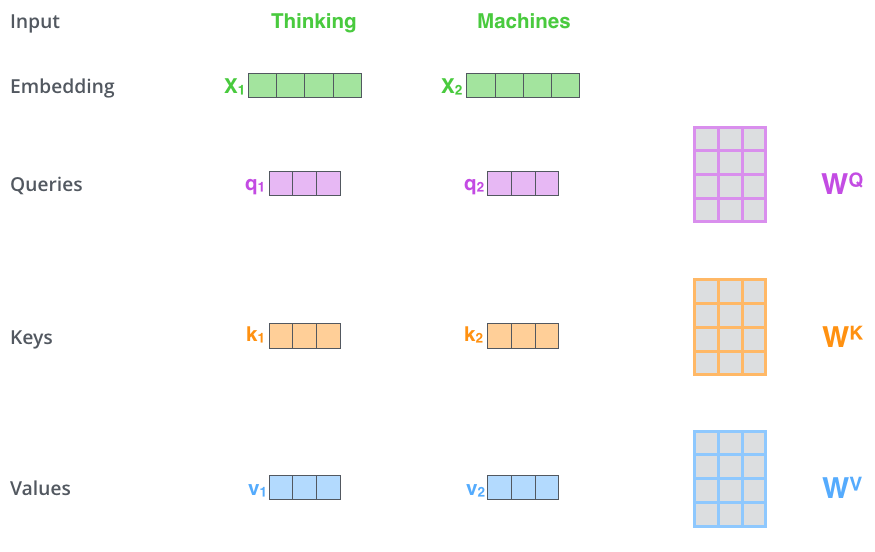
\includegraphics[width=\linewidth,keepaspectratio]{transformer_self_attention_vectors_jay}


{\tiny (Ref: ``The Illustrated Transformer'' - Jay Alammar)}
\end{center}		

		\end{column}
    \begin{column}[T]{0.5\linewidth}

\begin{itemize}
\item Create three vectors from each of the encoder’s input vectors (in this case, the embedding of each word). 
\item So for each word, we create a Query vector, a Key vector, and a Value vector. \item These vectors are created by multiplying the embedding by three matrices, which are trained during the training process.
\end{itemize}
    \end{column}
  \end{columns}
  
  Multiplying $x_1$ by the $W^Q$ weight matrix produces $q_1$, the ``query`` vector associated with that word. We end up creating a ``query'', a ``key'', and a ``value'' projection of each word in the input sentence.
  
  Note: new vectors are smaller, 64, while the embedding and encoder input/output vectors have dimensionality of 512. They don’t HAVE to be smaller, just a choice.
\end{frame}

%%%%%%%%%%%%%%%%%%%%%%%%%%%%%%%%%%%%%%%%%%%%%%%%%%%%%%%%%%%
\begin{frame}[fragile]\frametitle{Self-Attention Scores}

\begin{columns}
    \begin{column}[T]{0.5\linewidth}
\begin{center}
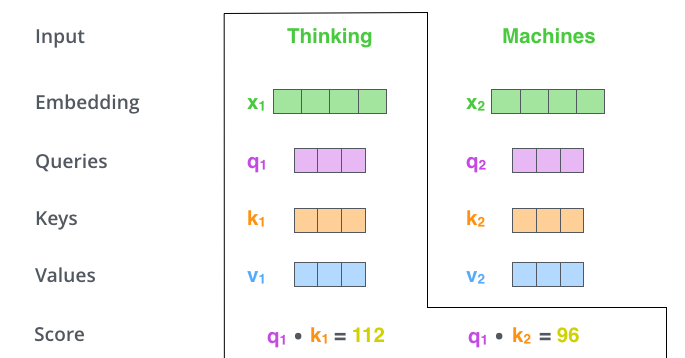
\includegraphics[width=\linewidth,keepaspectratio]{transformer_self_attention_score_jay}


{\tiny (Ref: ``The Illustrated Transformer'' - Jay Alammar)}
\end{center}		

		\end{column}
    \begin{column}[T]{0.5\linewidth}

\begin{itemize}
\item Calculating the self-attention for the first word in this example, ``Thinking''. 
\item Need to score each word of the input sentence against this word, thats its importance wrt that word
\item score = dot product of words query vector with key vector of the running words. Each is a single scalar value. So, score for first word $w_1, s_1 = q_1 k_1 + q_1 k_2 + \ldots$
\end{itemize}
    \end{column}
  \end{columns}

* Please note that in the diagram the Embedding vectors also include positional encoding incorporated inside.
\end{frame}

%%%%%%%%%%%%%%%%%%%%%%%%%%%%%%%%%%%%%%%%%%%%%%%%%%%%%%%%%%%
\begin{frame}[fragile]\frametitle{Self-Attention Scores}

\begin{columns}
    \begin{column}[T]{0.5\linewidth}
\begin{center}
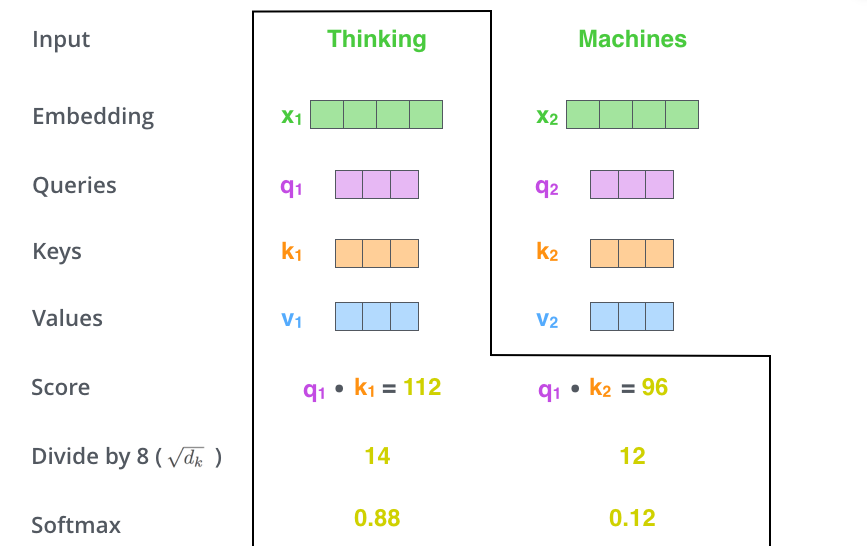
\includegraphics[width=\linewidth,keepaspectratio]{self-attention_softmax_jay}


{\tiny (Ref: ``The Illustrated Transformer'' - Jay Alammar)}
\end{center}		

		\end{column}
    \begin{column}[T]{0.5\linewidth}

\begin{itemize}
\item Divide the scores by 8 (the square root of the dimension of the key vectors used in the paper – 64. 
\item This leads to having more stable gradients. There could be other possible values here, but this is the default), 
\item then pass the result through a softmax that normalizes from 0 to 1

\end{itemize}
    \end{column}
  \end{columns}
  
   Note: Clearly word with itself will have the highest softmax score, thats ok
 but then next matching-high scores have importance

* Please note that in the diagram the Embedding vectors also include positional encoding incorporated inside.
\end{frame}

%%%%%%%%%%%%%%%%%%%%%%%%%%%%%%%%%%%%%%%%%%%%%%%%%%%%%%%%%%%
\begin{frame}[fragile]\frametitle{Self-Attention Scores with Value Vectors}

\begin{columns}
    \begin{column}[T]{0.5\linewidth}
\begin{center}
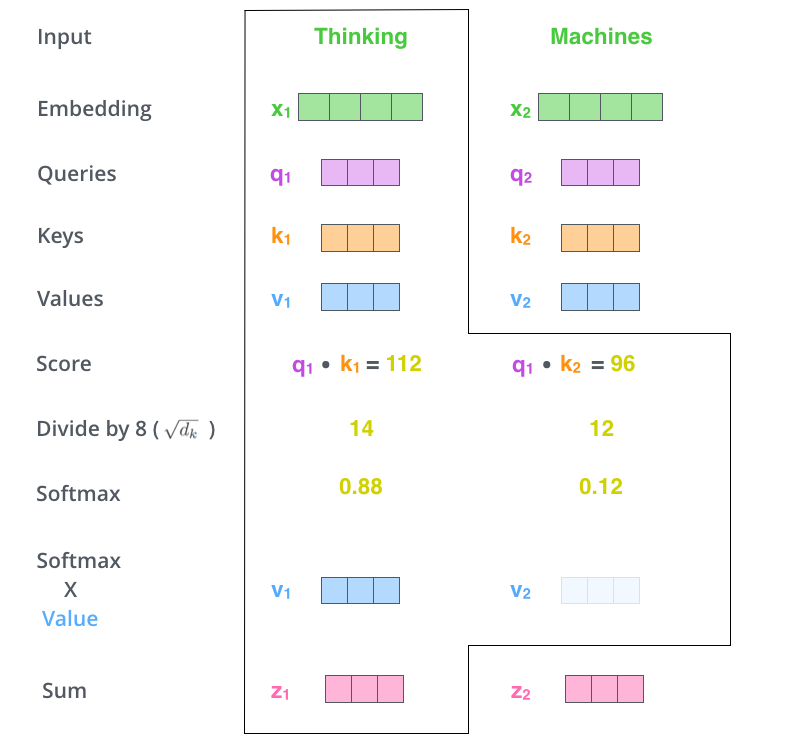
\includegraphics[width=\linewidth,keepaspectratio]{self-attention-output_jay}


{\tiny (Ref: ``The Illustrated Transformer'' - Jay Alammar)}
\end{center}		

		\end{column}
    \begin{column}[T]{0.5\linewidth}

\begin{itemize}
\item Multiply each value vector by the softmax scores respectively, like $s_1 \times v_1$ and $s_2 \times v_2$, here $s$s are scalars scores or weights, where as $v$s are value vectors.
\item The intuition here is to keep intact the values of the word(s) we want to focus on, and drown-out irrelevant words, basically weighted per position.
\item The last step is to sum up the weighted value vectors.
\item This produces the output of the self-attention layer at this position (for the first word).
\end{itemize}
    \end{column}
  \end{columns}

* Please note that in the diagram the Embedding vectors also include positional encoding incorporated inside.
\end{frame}

%%%%%%%%%%%%%%%%%%%%%%%%%%%%%%%%%%%%%%%%%%%%%%%%%%%%%%%%%%%
\begin{frame}[fragile]\frametitle{Self-Attention Scores in a Matrix Way}

\begin{columns}
    \begin{column}[T]{0.5\linewidth}
\begin{center}
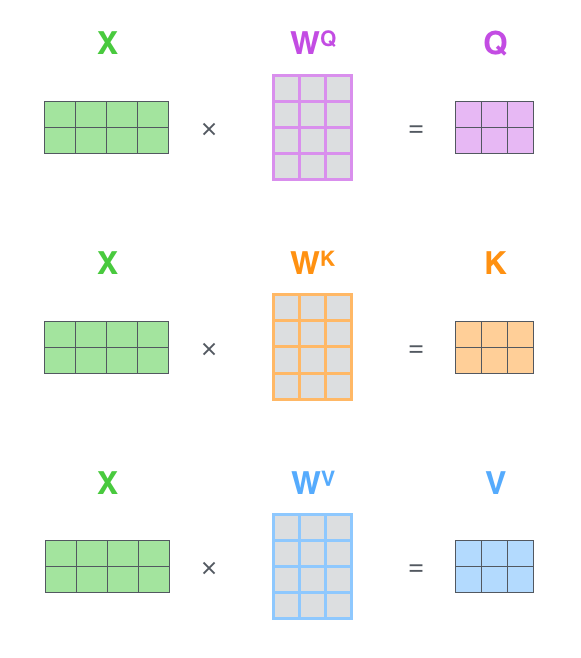
\includegraphics[width=0.8\linewidth,keepaspectratio]{self-attention-matrix-calculation_jay}


{\tiny (Ref: ``The Illustrated Transformer'' - Jay Alammar)}
\end{center}		

		\end{column}
    \begin{column}[T]{0.5\linewidth}

\begin{itemize}
\item Assuming two words in the sentence, so number of rows are two, num columns are 512 (but shown 4 just for brevity) and the q/k/v vectors (64, or 3 boxes in the figure)
\item  Calculate the Query, Key, and Value matrices. 
\item Input sentence vector is matrix $X$, and multiplying it by the weight matrices to be trained ($W^Q, W^K, W^V$).
\end{itemize}
    \end{column}
  \end{columns}

* Please note that in the diagram the Embedding vectors $X$ also include positional encoding incorporated inside.
\end{frame}

%%%%%%%%%%%%%%%%%%%%%%%%%%%%%%%%%%%%%%%%%%%%%%%%%%%%%%%%%%%
\begin{frame}[fragile]\frametitle{Self-Attention Scores in a single formula}


\begin{center}
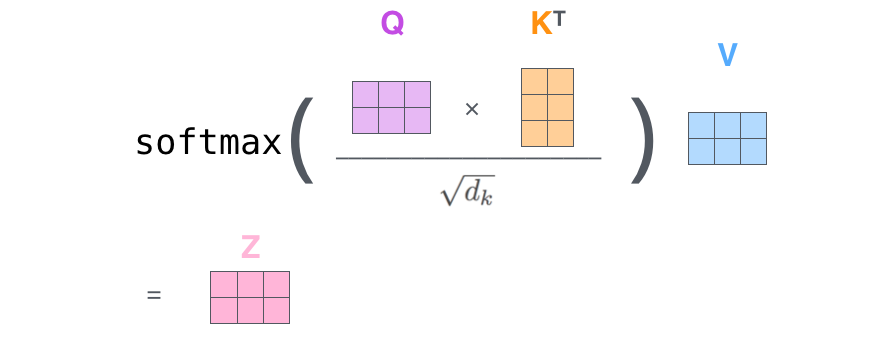
\includegraphics[width=\linewidth,keepaspectratio]{self-attention-matrix-calculation-2_jay}


{\tiny (Ref: ``The Illustrated Transformer'' - Jay Alammar)}
\end{center}		

\end{frame}



% %%%%%%%%%%%%%%%%%%%%%%%%%%%%%%%%%%%%%%%%%%%%%%%%%%%%%%%%%%%
% \begin{frame}[fragile]\frametitle{Self Attention Summary}


% \begin{center}
% 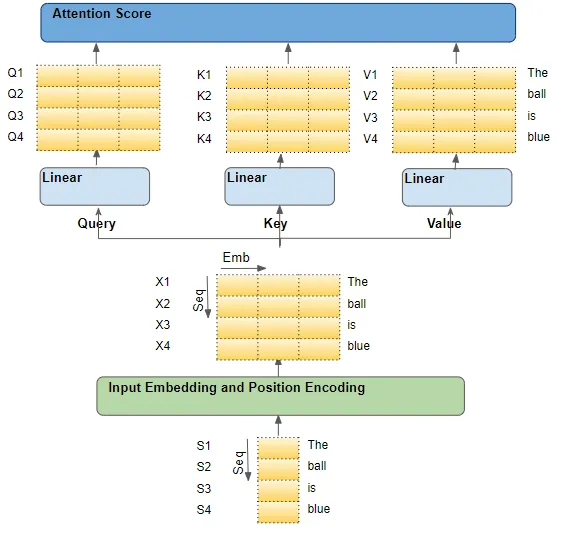
\includegraphics[width=0.6\linewidth,keepaspectratio]{transformer_self_attention_summary}


% {\tiny (Ref: ``Transformers Explained Visually (Part 1): Overview of Functionality'' - Ketan Doshi)}
% \end{center}		


% \end{frame}


% %%%%%%%%%%%%%%%%%%%%%%%%%%%%%%%%%%%%%%%%%%%%%%%%%%%%%%%%%%%
% \begin{frame}[fragile]\frametitle{Dot-Product Attention}


      % \begin{itemize}
			% \item Inputs: a query q and a set of key-value (k-v) pairs to an output
			% \item Query, keys, values, and output are all vectors
			% \item Output is weighted sum of values, where
			% \item Weight of each value is computed by an inner product of query and corresponding key
			% \item Queries and keys have same dimensionality $d_k$ , value have $d_v$
			% \end{itemize}
			
			% \begin{center}
			% 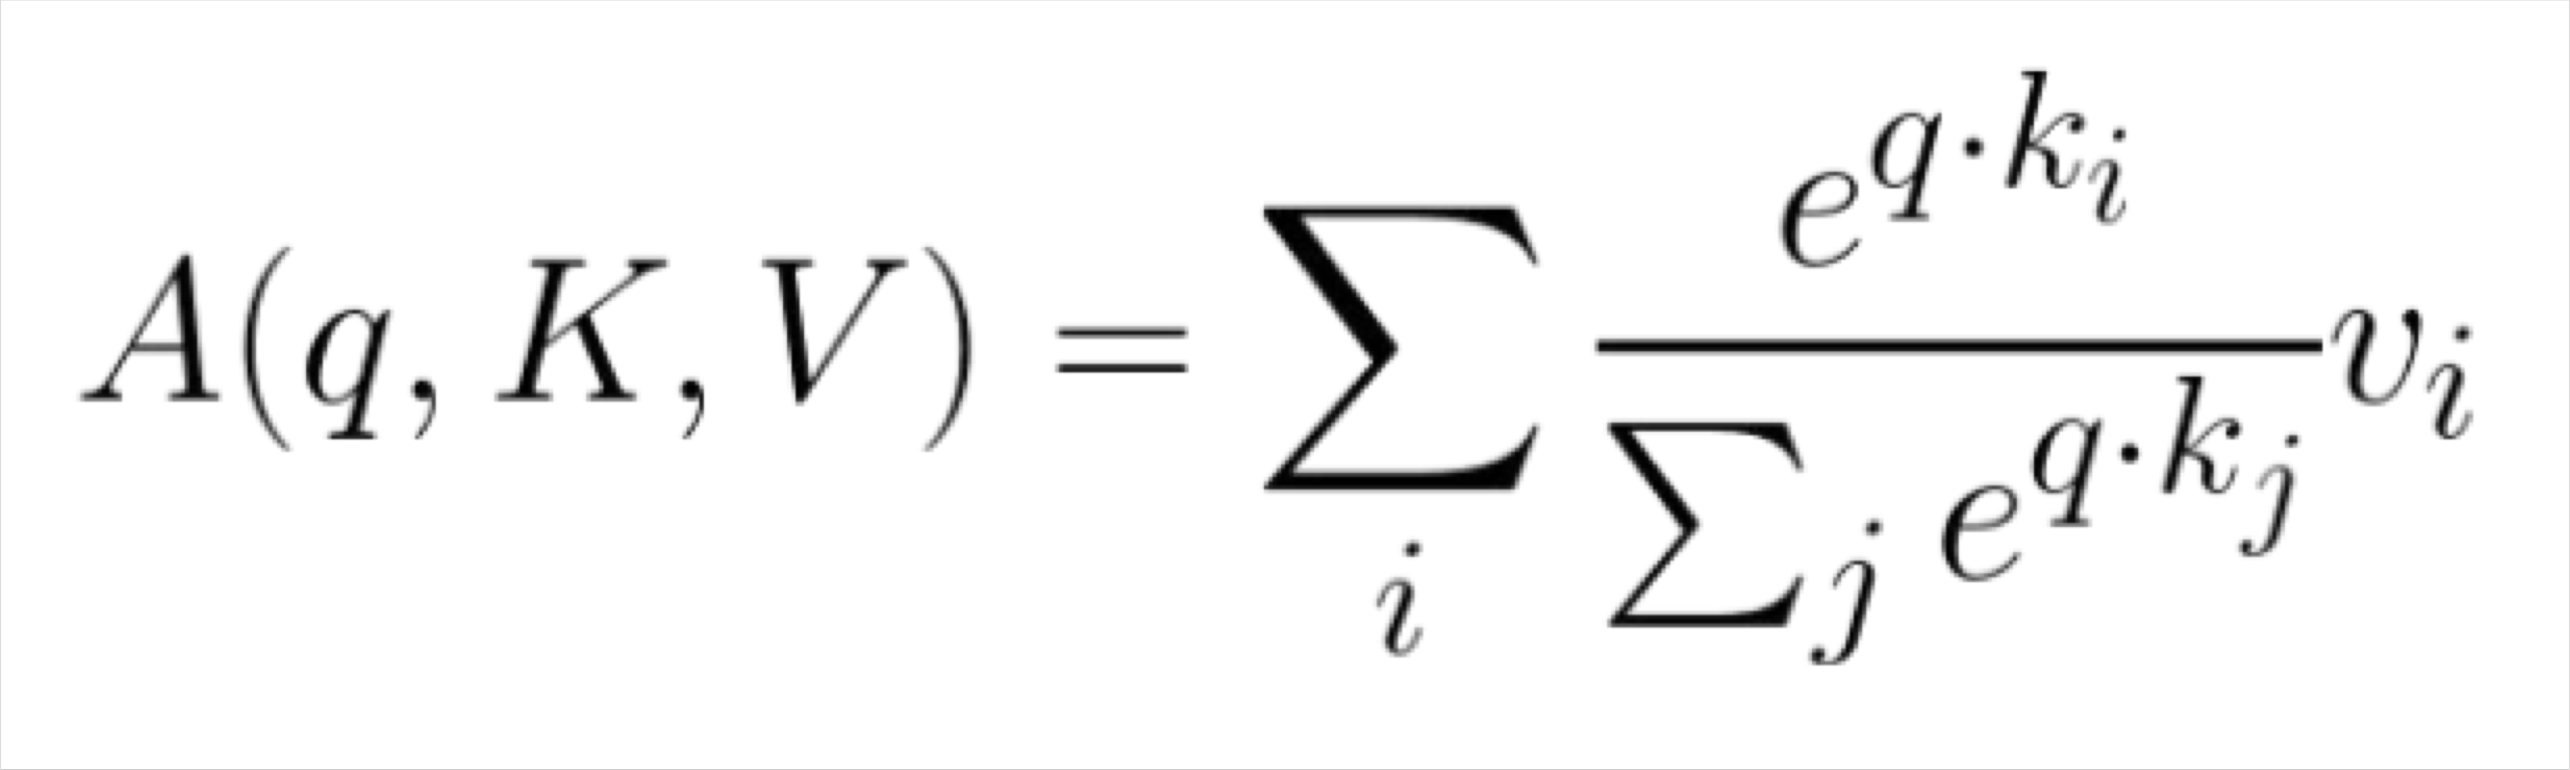
\includegraphics[width=0.4\linewidth,keepaspectratio]{bert73}
			% \end{center}		
			
			% % {\tiny (Ref: CS224n: Natural Language Processing with Deep Learning - Christopher Manning)}

% \end{frame}

% %%%%%%%%%%%%%%%%%%%%%%%%%%%%%%%%%%%%%%%%%%%%%%%%%%%%%%%%%%%
% \begin{frame}[fragile]\frametitle{Matrix notation}


      % \begin{itemize}
			% \item Inputs: a query q and a set of key-value (k-v) pairs to an output
			% \item Query, keys, values, and output are all vectors
			% \item Output is weighted sum of values, where
			% \item Weight of each value is computed by an inner product of query and corresponding key
			% \item Queries and keys have same dimensionality $d_k$ , value have $d_v$
			% \end{itemize}
			
			% \begin{center}
			% 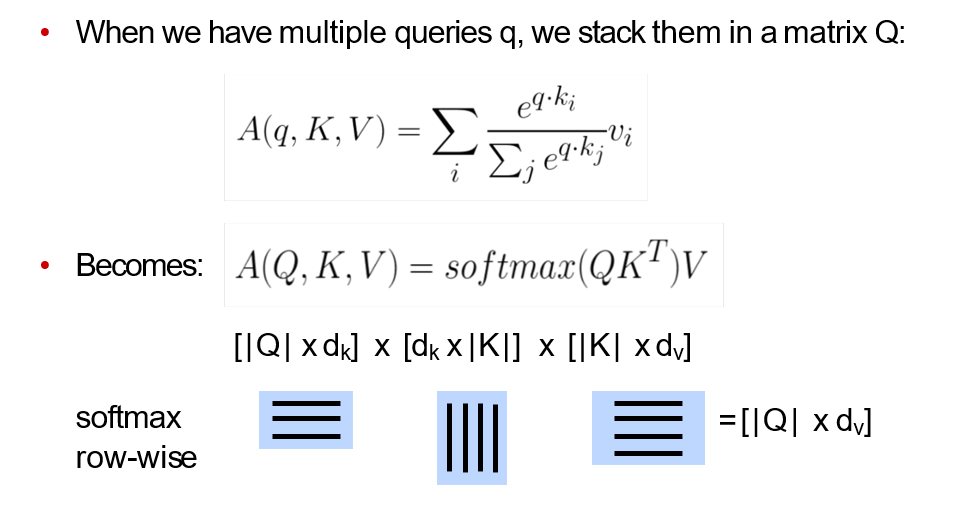
\includegraphics[width=0.8\linewidth,keepaspectratio]{bert74}
			% \end{center}		
			
			% % {\tiny (Ref: CS224n: Natural Language Processing with Deep Learning - Christopher Manning)}

% \end{frame}

% %%%%%%%%%%%%%%%%%%%%%%%%%%%%%%%%%%%%%%%%%%%%%%%%%%%%%%%%%%%
% \begin{frame}[fragile]\frametitle{Key-Query-Value Attention}

			
			% \begin{center}
			% 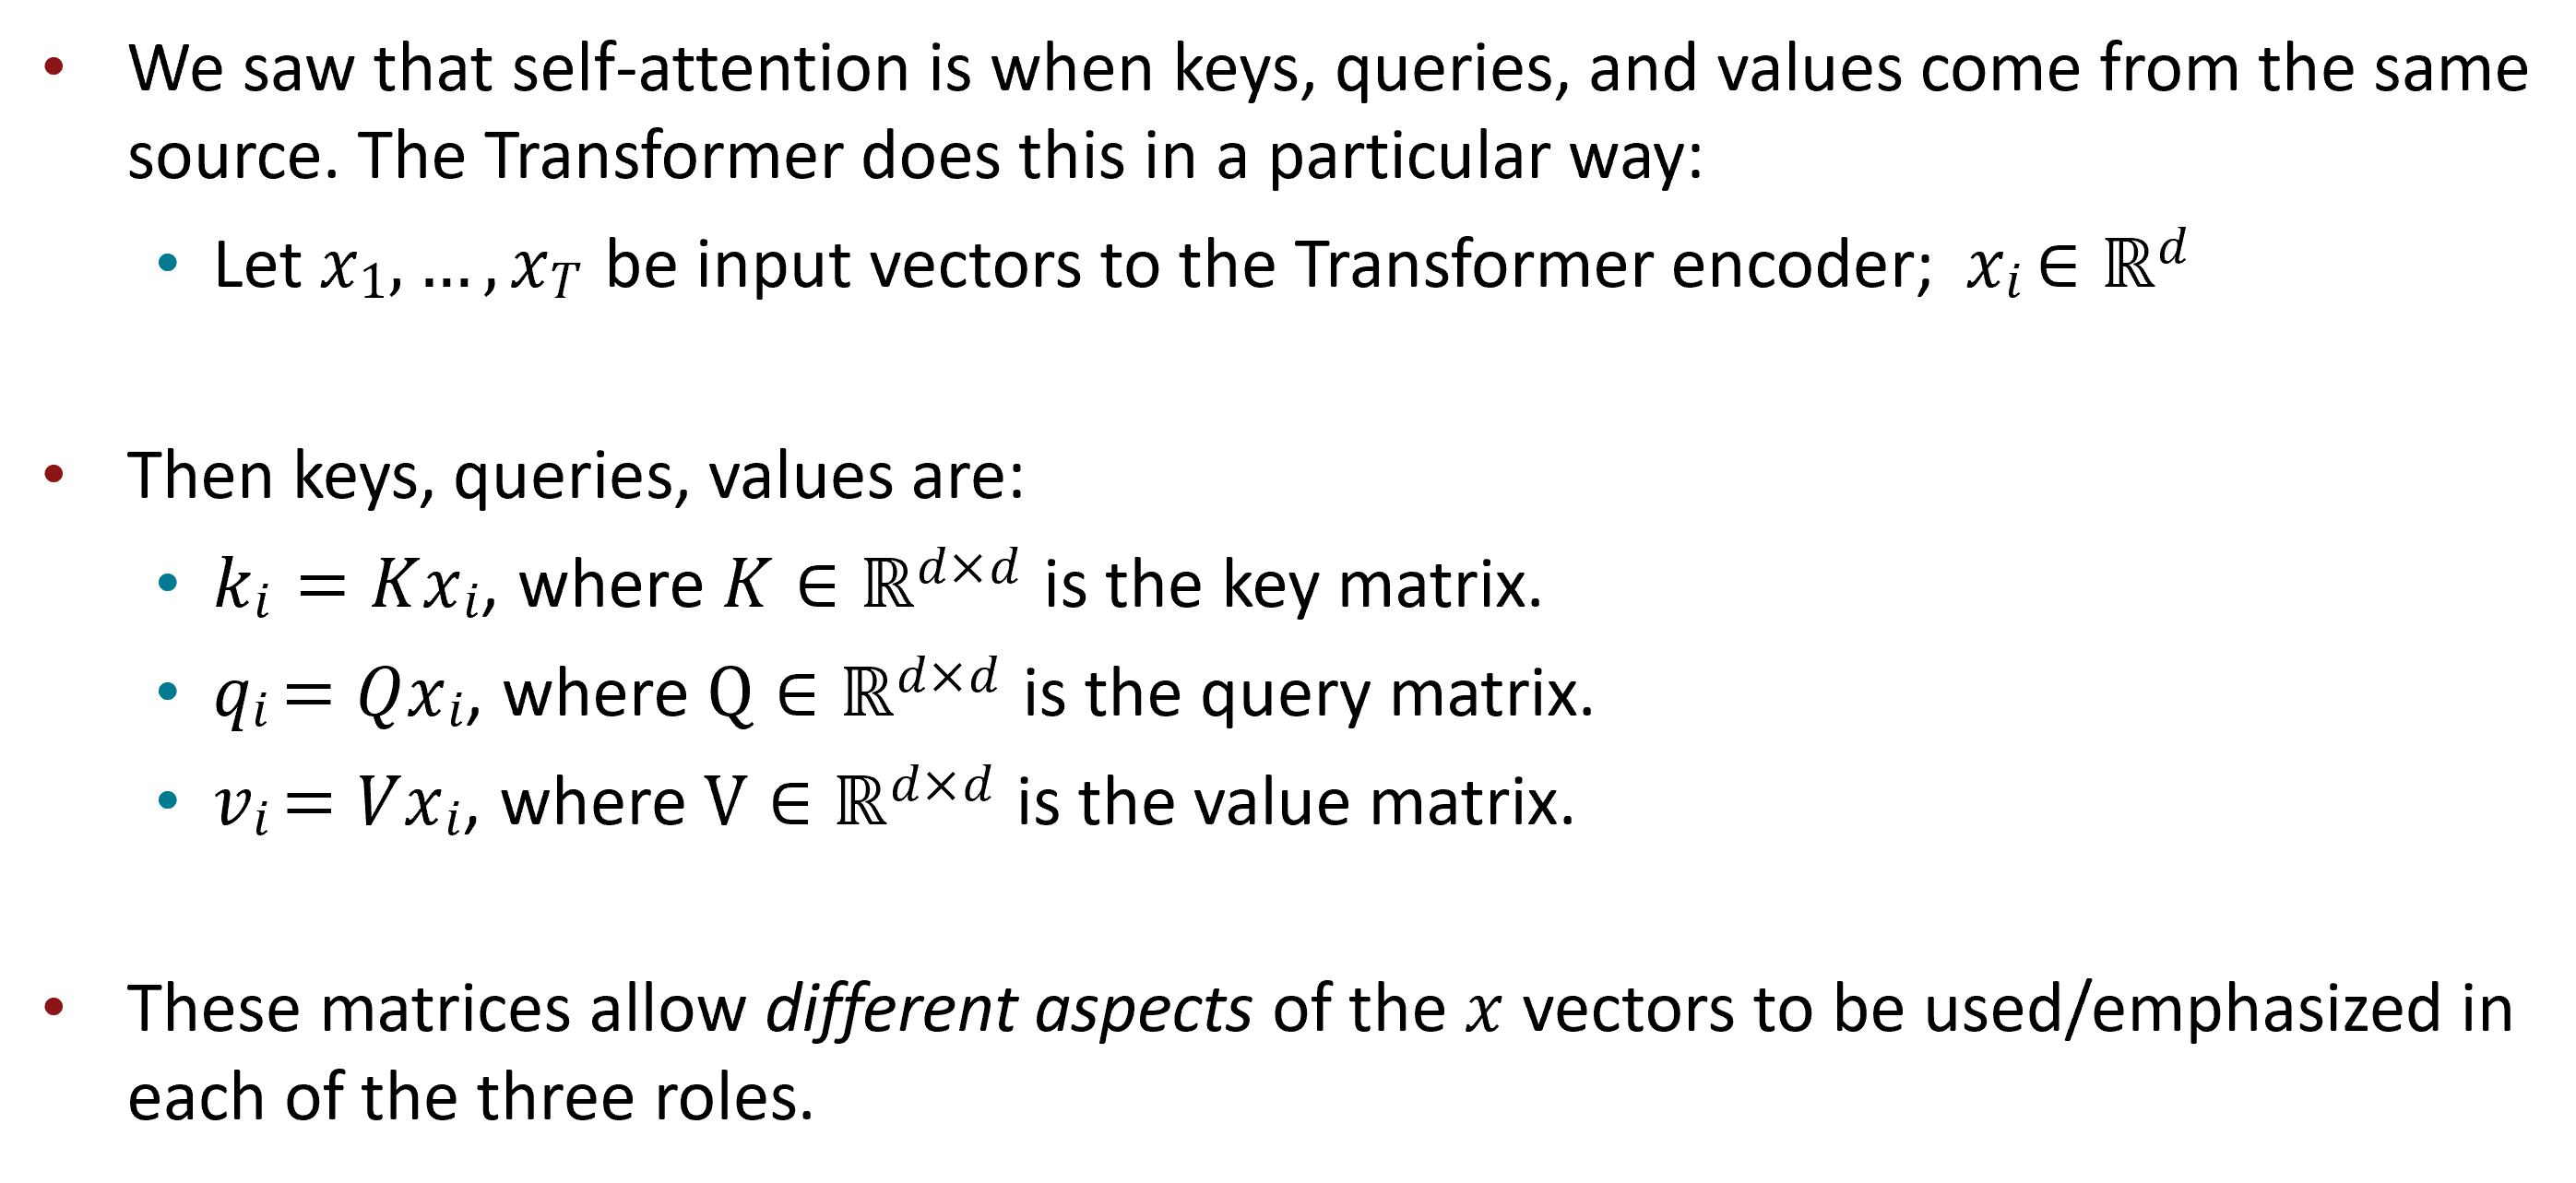
\includegraphics[width=\linewidth,keepaspectratio]{bert75}
			% \end{center}		
			
% % {\tiny (Ref: Language \& Machine Learning - John Hewitt)}

% \end{frame}

% %%%%%%%%%%%%%%%%%%%%%%%%%%%%%%%%%%%%%%%%%%%%%%%%%%%%%%%%%%%
% \begin{frame}[fragile]\frametitle{Key-Query-Value Attention}

			
			% \begin{center}
			% 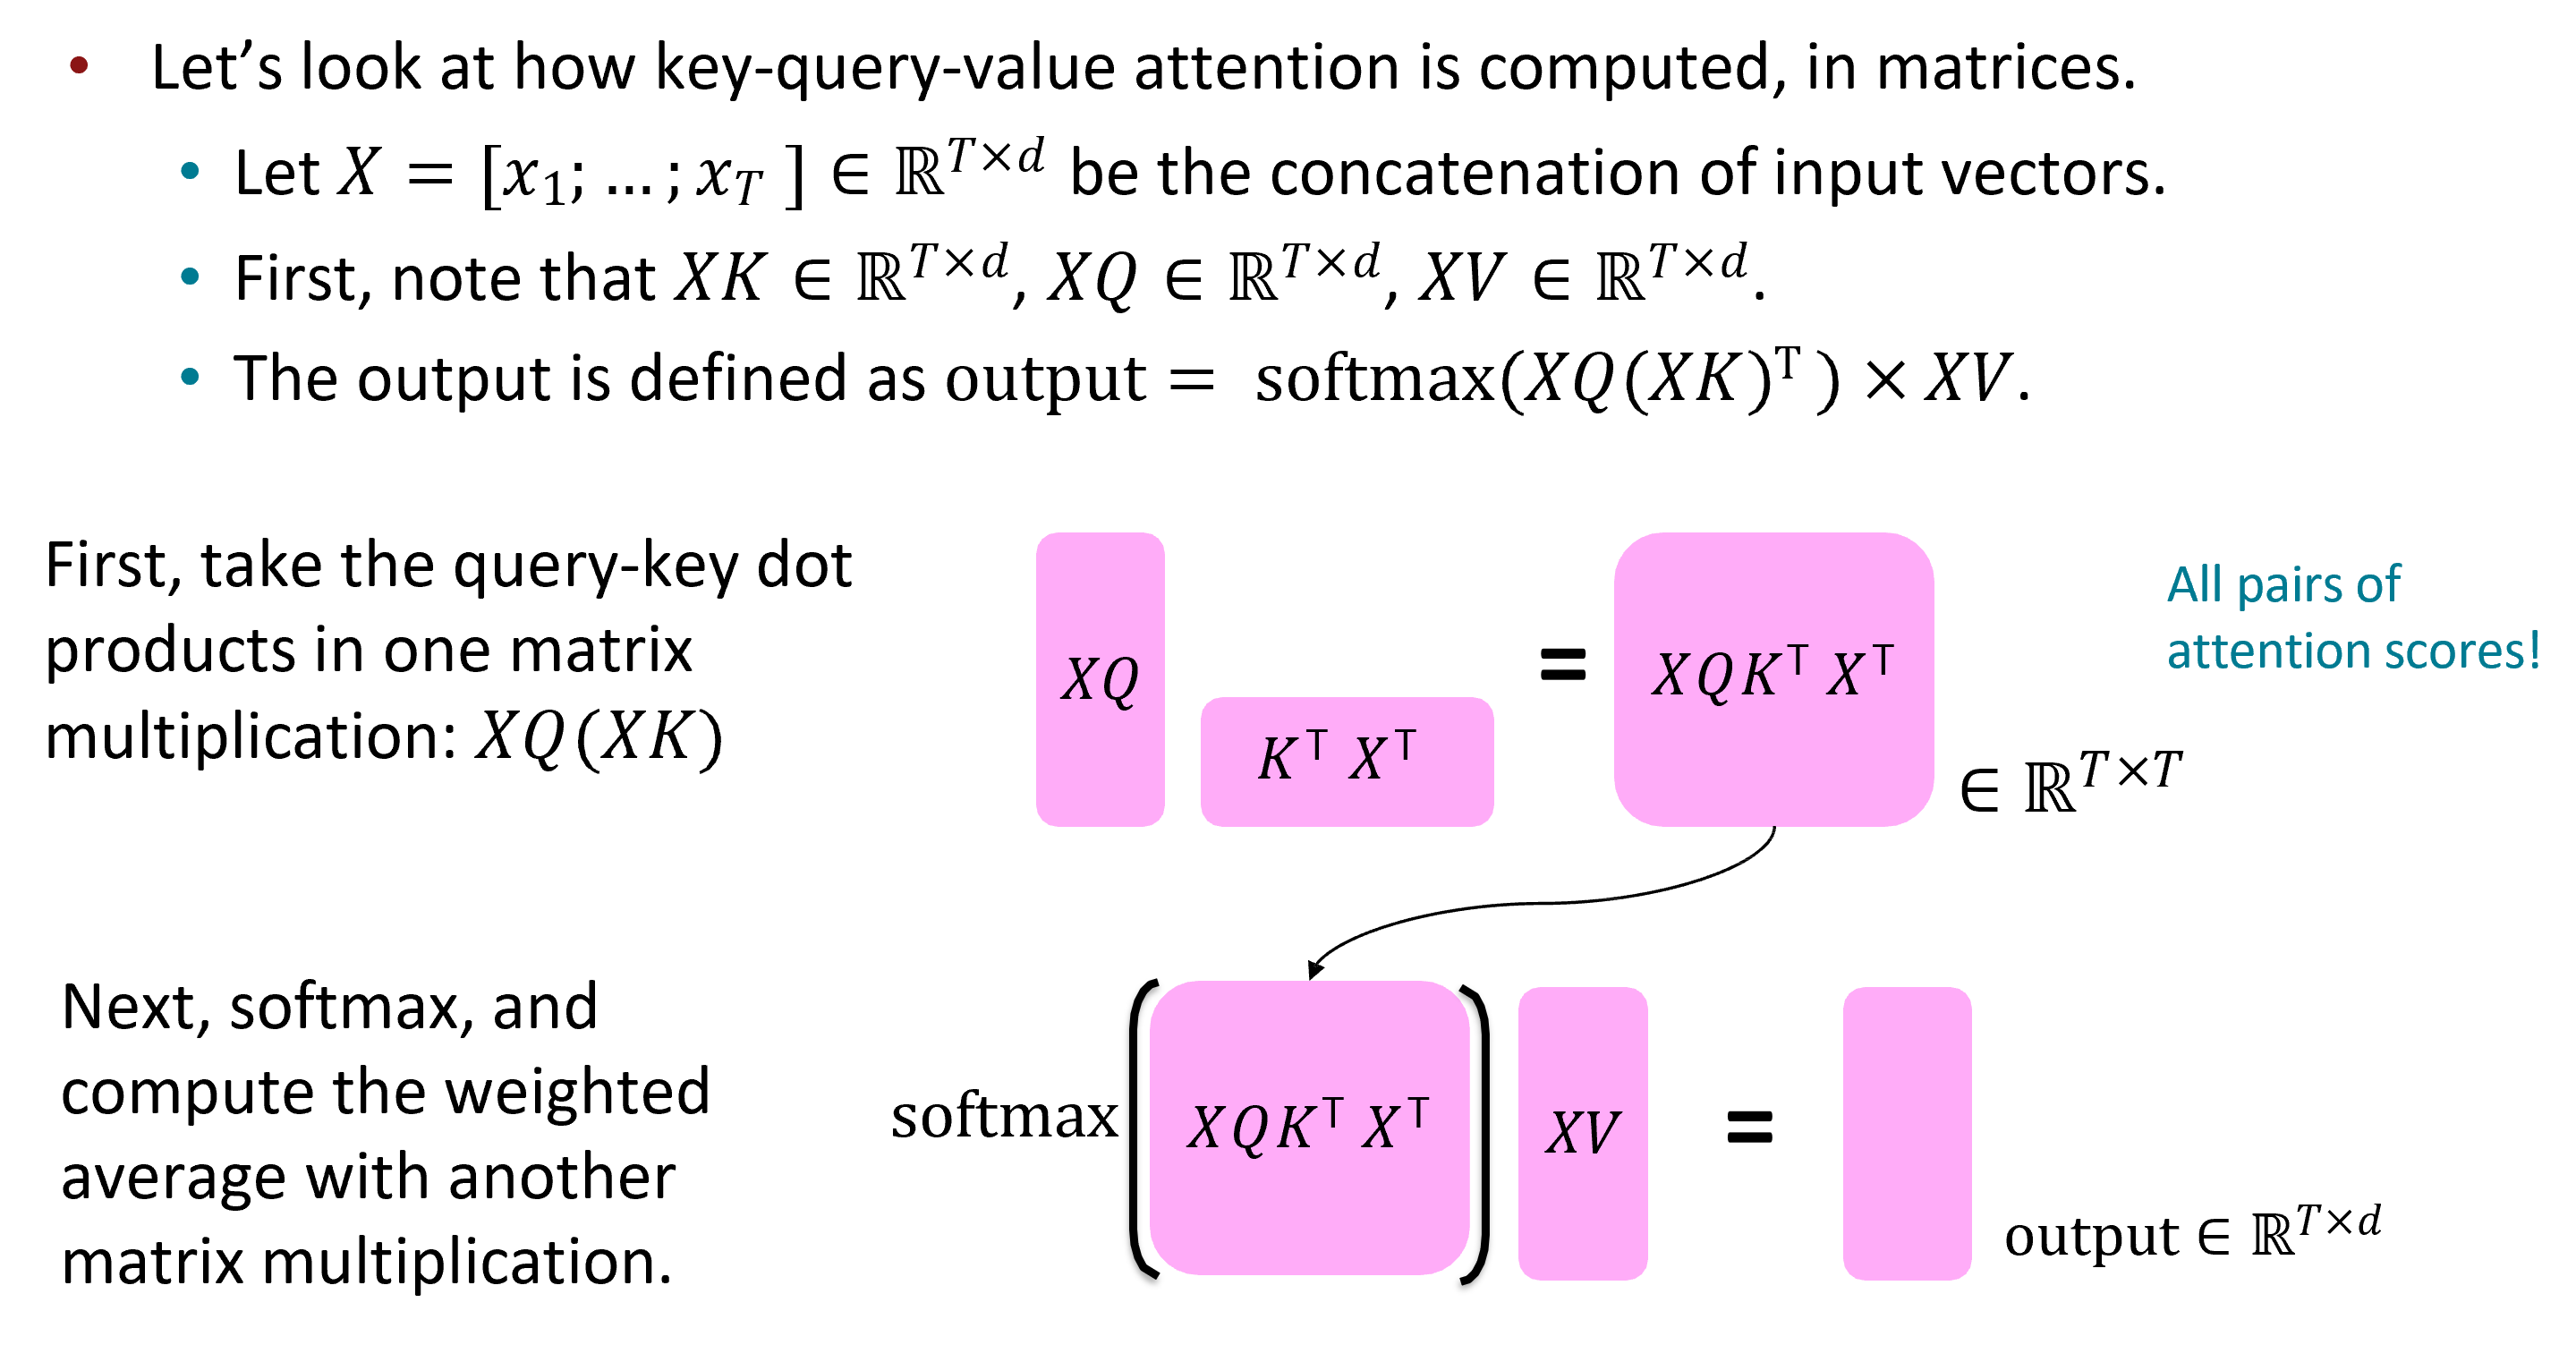
\includegraphics[width=\linewidth,keepaspectratio]{bert76}
			% \end{center}		
			
% % {\tiny (Ref: Language \& Machine Learning - John Hewitt)}

% \end{frame}


%%%%%%%%%%%%%%%%%%%%%%%%%%%%%%%%%%%%%%%%%%%%%%%%%%%%%%%%%%%%%%%%%%%%%%%%%%%%%%%%%%
\begin{frame}[fragile]\frametitle{}
\begin{center}
{\Large Multi-head Attention}
\end{center}
\end{frame}

%%%%%%%%%%%%%%%%%%%%%%%%%%%%%%%%%%%%%%%%%%%%%%%%%%%%%%%%%%%
\begin{frame}[fragile]\frametitle{The Beast With Many Heads}

Having multiple self attention helps:

\begin{columns}
    \begin{column}[T]{0.5\linewidth}
\begin{center}
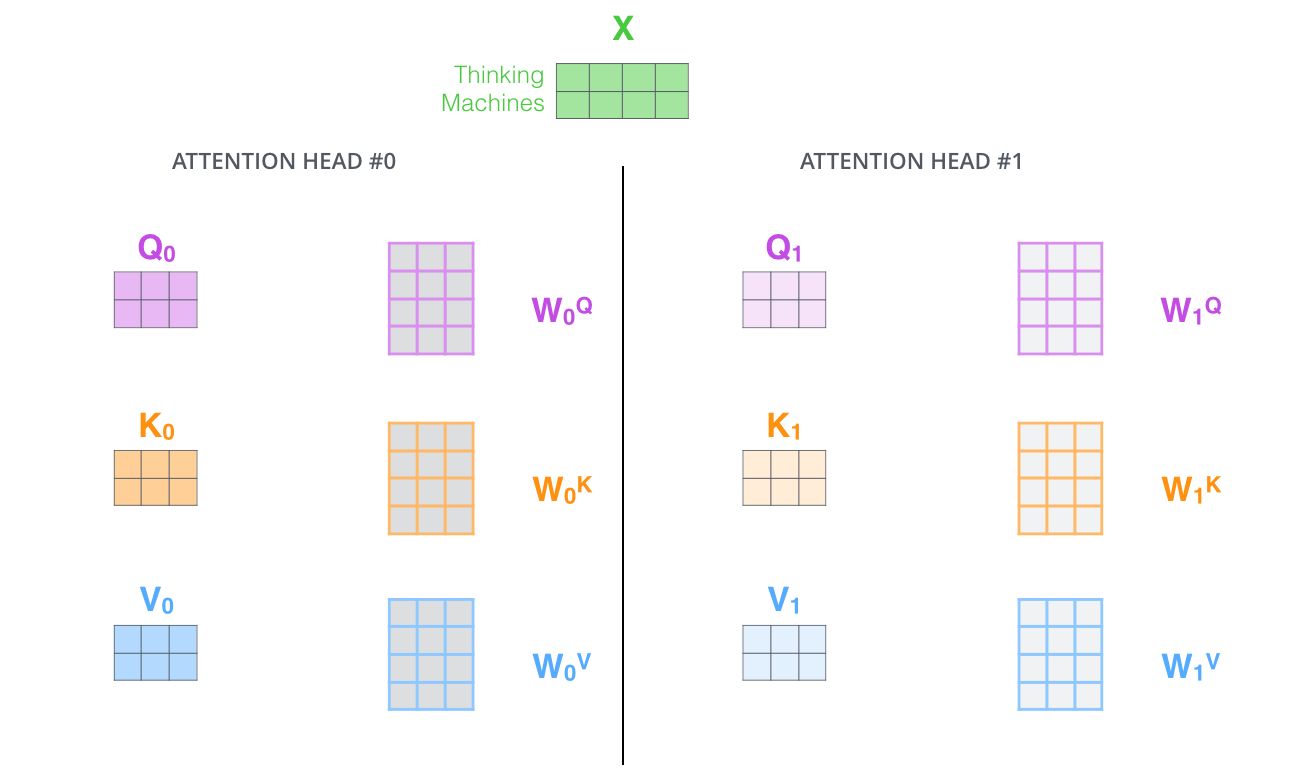
\includegraphics[width=\linewidth,keepaspectratio]{transformer_attention_heads_qkv_jay}


{\tiny (Ref: ``The Illustrated Transformer'' - Jay Alammar)}
\end{center}		

		\end{column}
    \begin{column}[T]{0.5\linewidth}

\begin{itemize}
\item Expands the model’s ability to focus on different positions. Because each weight matrices of Q K V are initialized randomly, they can get settled differently, and also differently for different sentences.
\item Paper uses 8 heads in a single multi-head self attention cell.
\item ie Each of these sets is randomly initialized. Then, after training, each set is used to project the input embeddings (or vectors from lower encoders/decoders) into a different representation subspace.
\end{itemize}
    \end{column}
  \end{columns}
\end{frame}

%%%%%%%%%%%%%%%%%%%%%%%%%%%%%%%%%%%%%%%%%%%%%%%%%%%%%%%%%%%
\begin{frame}[fragile]\frametitle{The Beast With Many Heads}

Having multiple self attention helps:

\begin{columns}
    \begin{column}[T]{0.5\linewidth}
\begin{center}
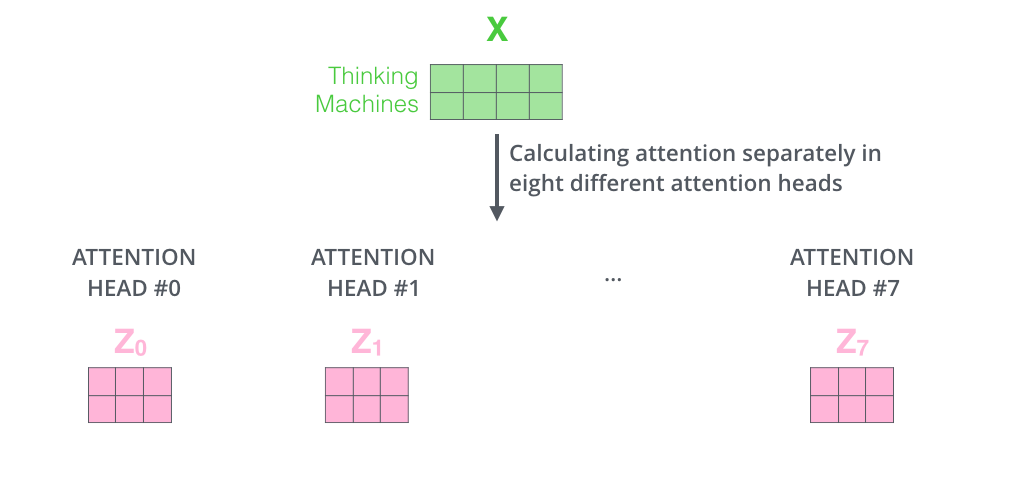
\includegraphics[width=\linewidth,keepaspectratio]{transformer_attention_heads_z_jay}


{\tiny (Ref: ``The Illustrated Transformer'' - Jay Alammar)}
\end{center}		

		\end{column}
    \begin{column}[T]{0.5\linewidth}

\begin{itemize}
\item One problem though. 
\item The next feed-forward layer is not expecting eight matrices – it’s expecting a single matrix (a vector for each word). So we need a way to condense these eight down into a single matrix.
\item How do we do that? 
\end{itemize}
    \end{column}
  \end{columns}
\end{frame}

%%%%%%%%%%%%%%%%%%%%%%%%%%%%%%%%%%%%%%%%%%%%%%%%%%%%%%%%%%%
\begin{frame}[fragile]\frametitle{The Beast With Many Heads}

Having multiple self attention helps:

\begin{columns}
    \begin{column}[T]{0.5\linewidth}
\begin{center}
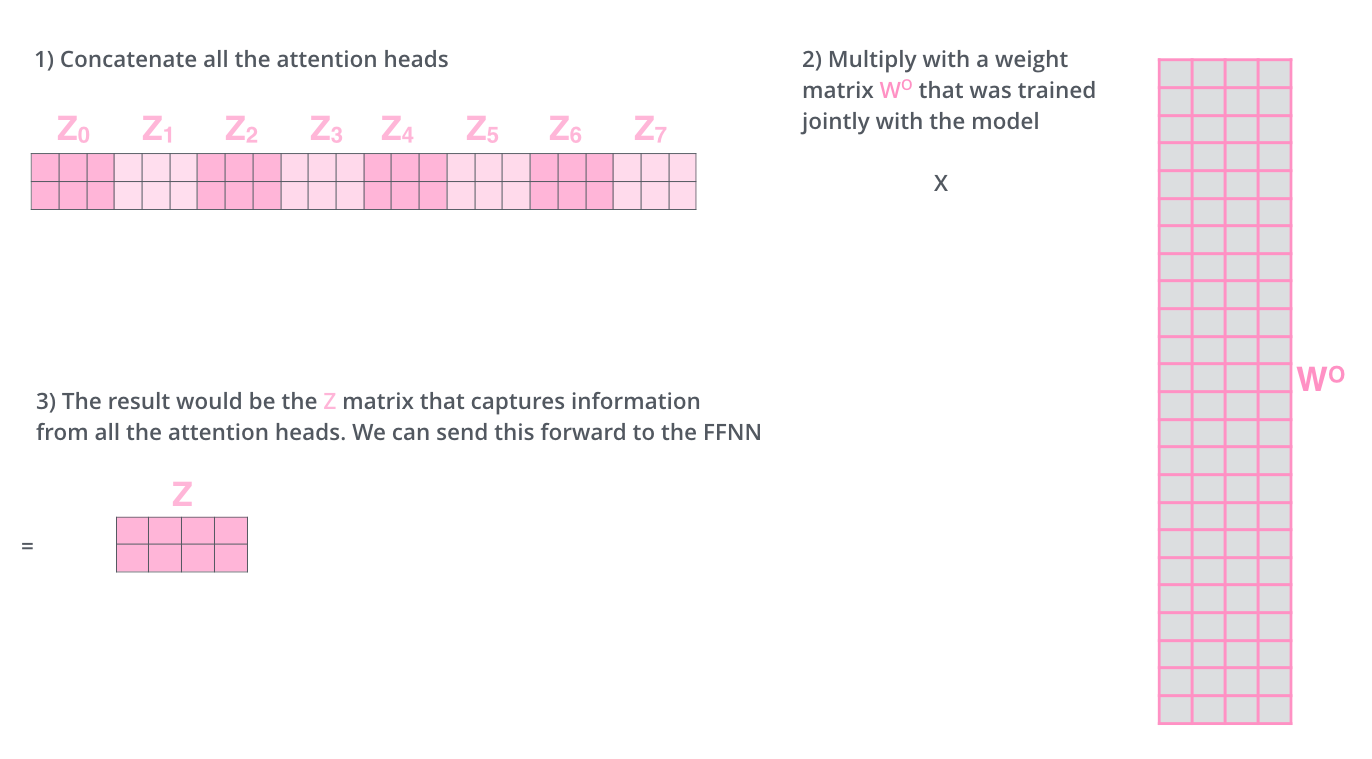
\includegraphics[width=\linewidth,keepaspectratio]{transformer_attention_heads_weight_matrix_o_jay}


{\tiny (Ref: ``The Illustrated Transformer'' - Jay Alammar)}
\end{center}		

		\end{column}
    \begin{column}[T]{0.5\linewidth}

\begin{itemize}
\item  We concat the matrices then multiply them by an additional weights matrix $W^O$.
\end{itemize}
    \end{column}
  \end{columns}
\end{frame}


%%%%%%%%%%%%%%%%%%%%%%%%%%%%%%%%%%%%%%%%%%%%%%%%%%%%%%%%%%%
\begin{frame}[fragile]\frametitle{Self Attention in Summary}


\begin{center}
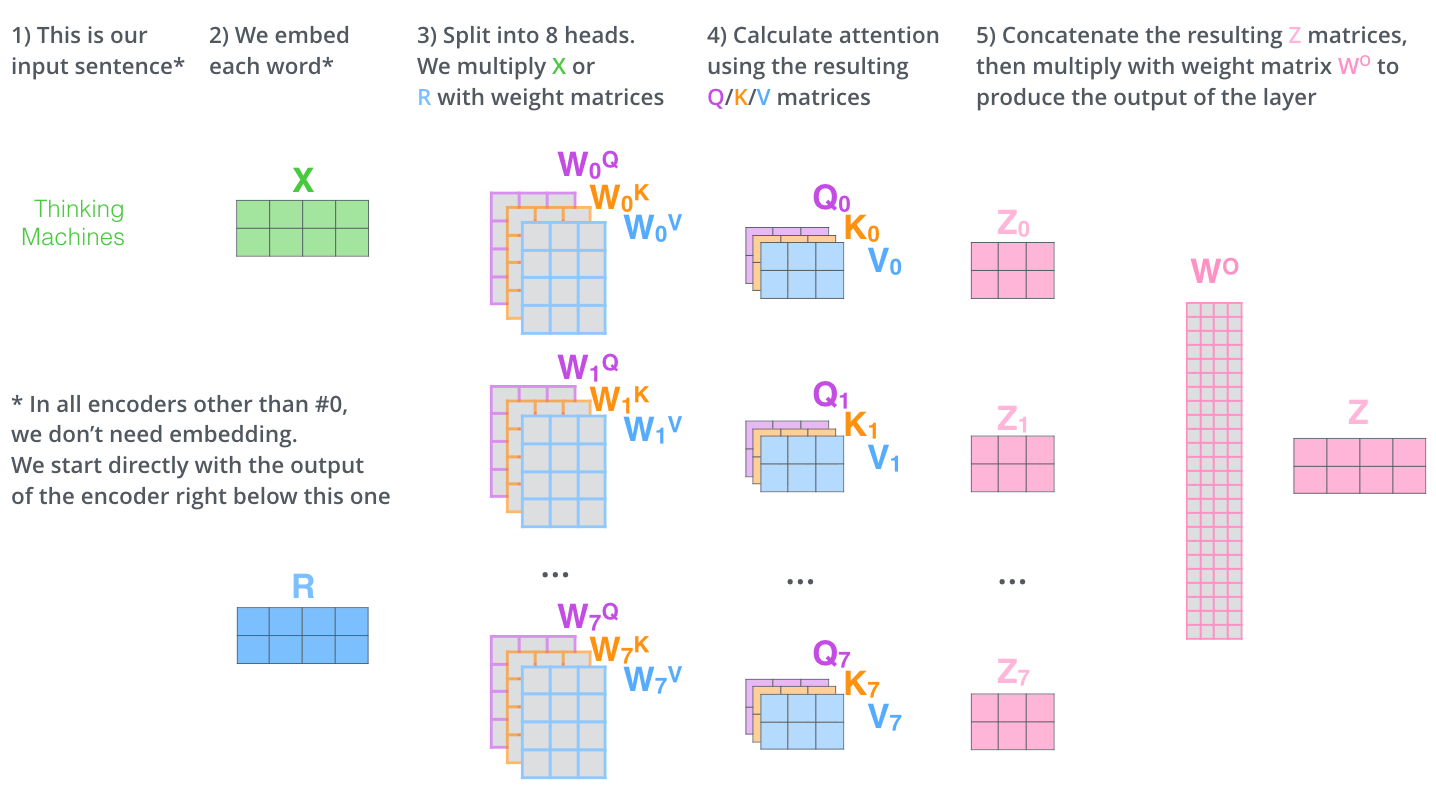
\includegraphics[width=\linewidth,keepaspectratio]{transformer_multi-headed_self-attention-recap_jay}


{\tiny (Ref: ``The Illustrated Transformer'' - Jay Alammar)}
\end{center}	


* Please note that in the diagram the Embedding vectors $X$ also include positional encoding incorporated inside.	$R$ shown in the diagram refers to output of previous encoder cell to the next one. First the first cell, its $X$, but for the subsequent ones, its the output of the previous cell, that's $R$.

\end{frame}


%%%%%%%%%%%%%%%%%%%%%%%%%%%%%%%%%%%%%%%%%%%%%%%%%%%%%%%%%%%
\begin{frame}[fragile]\frametitle{Self Attention in Summary Example}

\begin{columns}
    \begin{column}[T]{0.5\linewidth}
\begin{center}
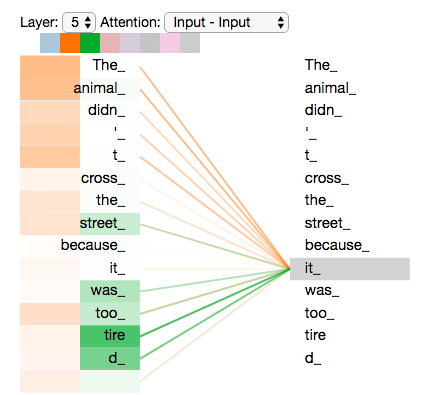
\includegraphics[width=\linewidth,keepaspectratio]{transformer_self-attention_visualization_2_jay}


{\tiny (Ref: ``The Illustrated Transformer'' - Jay Alammar)}
\end{center}	
		\end{column}
    \begin{column}[T]{0.5\linewidth}

As we encode the word "it", one attention head is focusing most on "the animal", while another is focusing on "tired" -- in a sense, the model's representation of the word "it" bakes in some of the representation of both "animal" and "tired".
    \end{column}
  \end{columns}
\end{frame}

%%%%%%%%%%%%%%%%%%%%%%%%%%%%%%%%%%%%%%%%%%%%%%%%%%%%%%%%%%%
\begin{frame}[fragile]\frametitle{Self Attention in Summary Example}

\begin{columns}
    \begin{column}[T]{0.5\linewidth}

\begin{center}
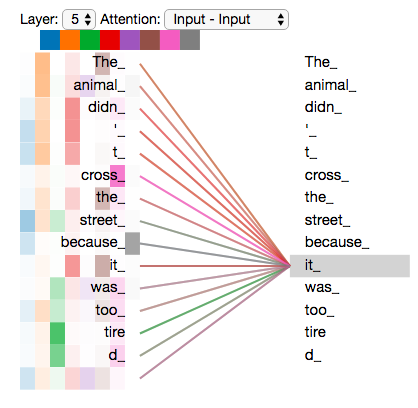
\includegraphics[width=\linewidth,keepaspectratio]{transformer_self-attention_visualization_3_jay}


{\tiny (Ref: ``The Illustrated Transformer'' - Jay Alammar)}
\end{center}	
		\end{column}
    \begin{column}[T]{0.5\linewidth}
If we add all the attention heads to the picture, however, things can be harder to interpret, but thats what happens.

This is how Self-Attention block generates, ``attended'' vectors.
    \end{column}
  \end{columns}
\end{frame}

% %%%%%%%%%%%%%%%%%%%%%%%%%%%%%%%%%%%%%%%%%%%%%%%%%%%%%%%%%%%
% \begin{frame}[fragile]\frametitle{Multi-headed attention}

			
			% \begin{center}
			% 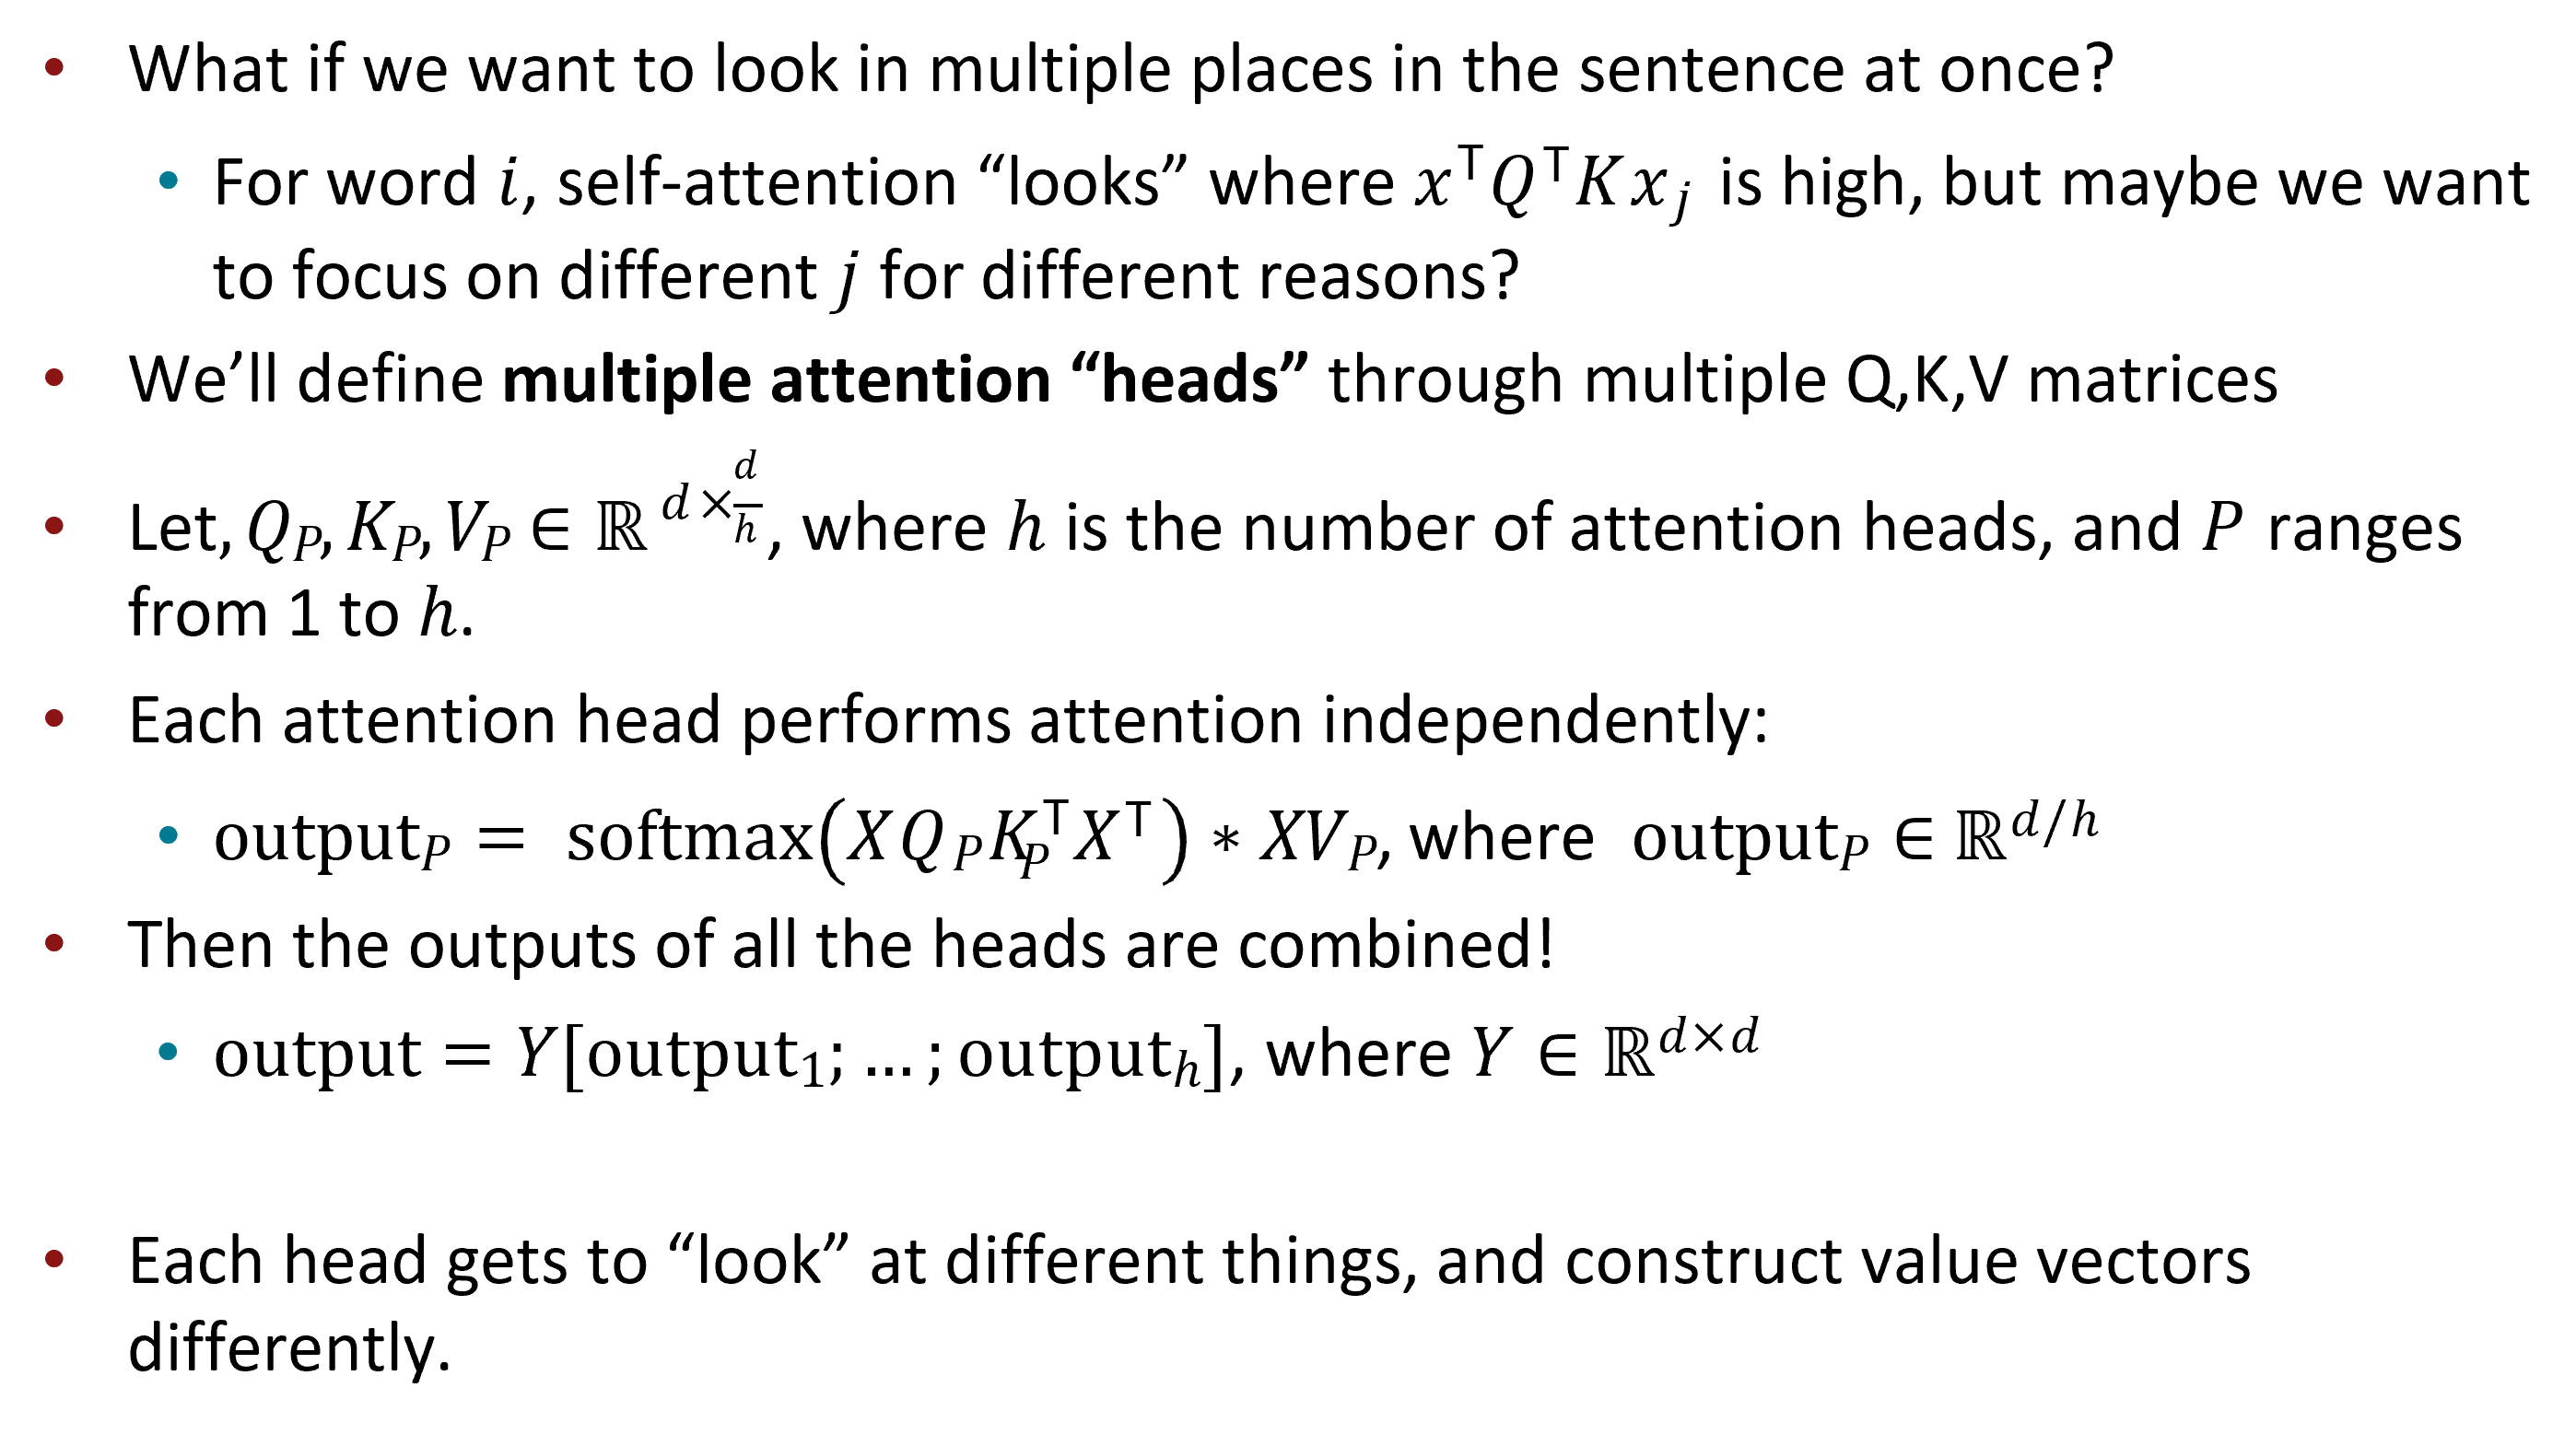
\includegraphics[width=\linewidth,keepaspectratio]{bert77}
			% \end{center}		
			
% % {\tiny (Ref: Language \& Machine Learning - John Hewitt)}

% \end{frame}

% %%%%%%%%%%%%%%%%%%%%%%%%%%%%%%%%%%%%%%%%%%%%%%%%%%%%%%%%%%%
% \begin{frame}[fragile]\frametitle{The Transformer Encoder: Multi-headed attention}

			
			% \begin{center}
			% 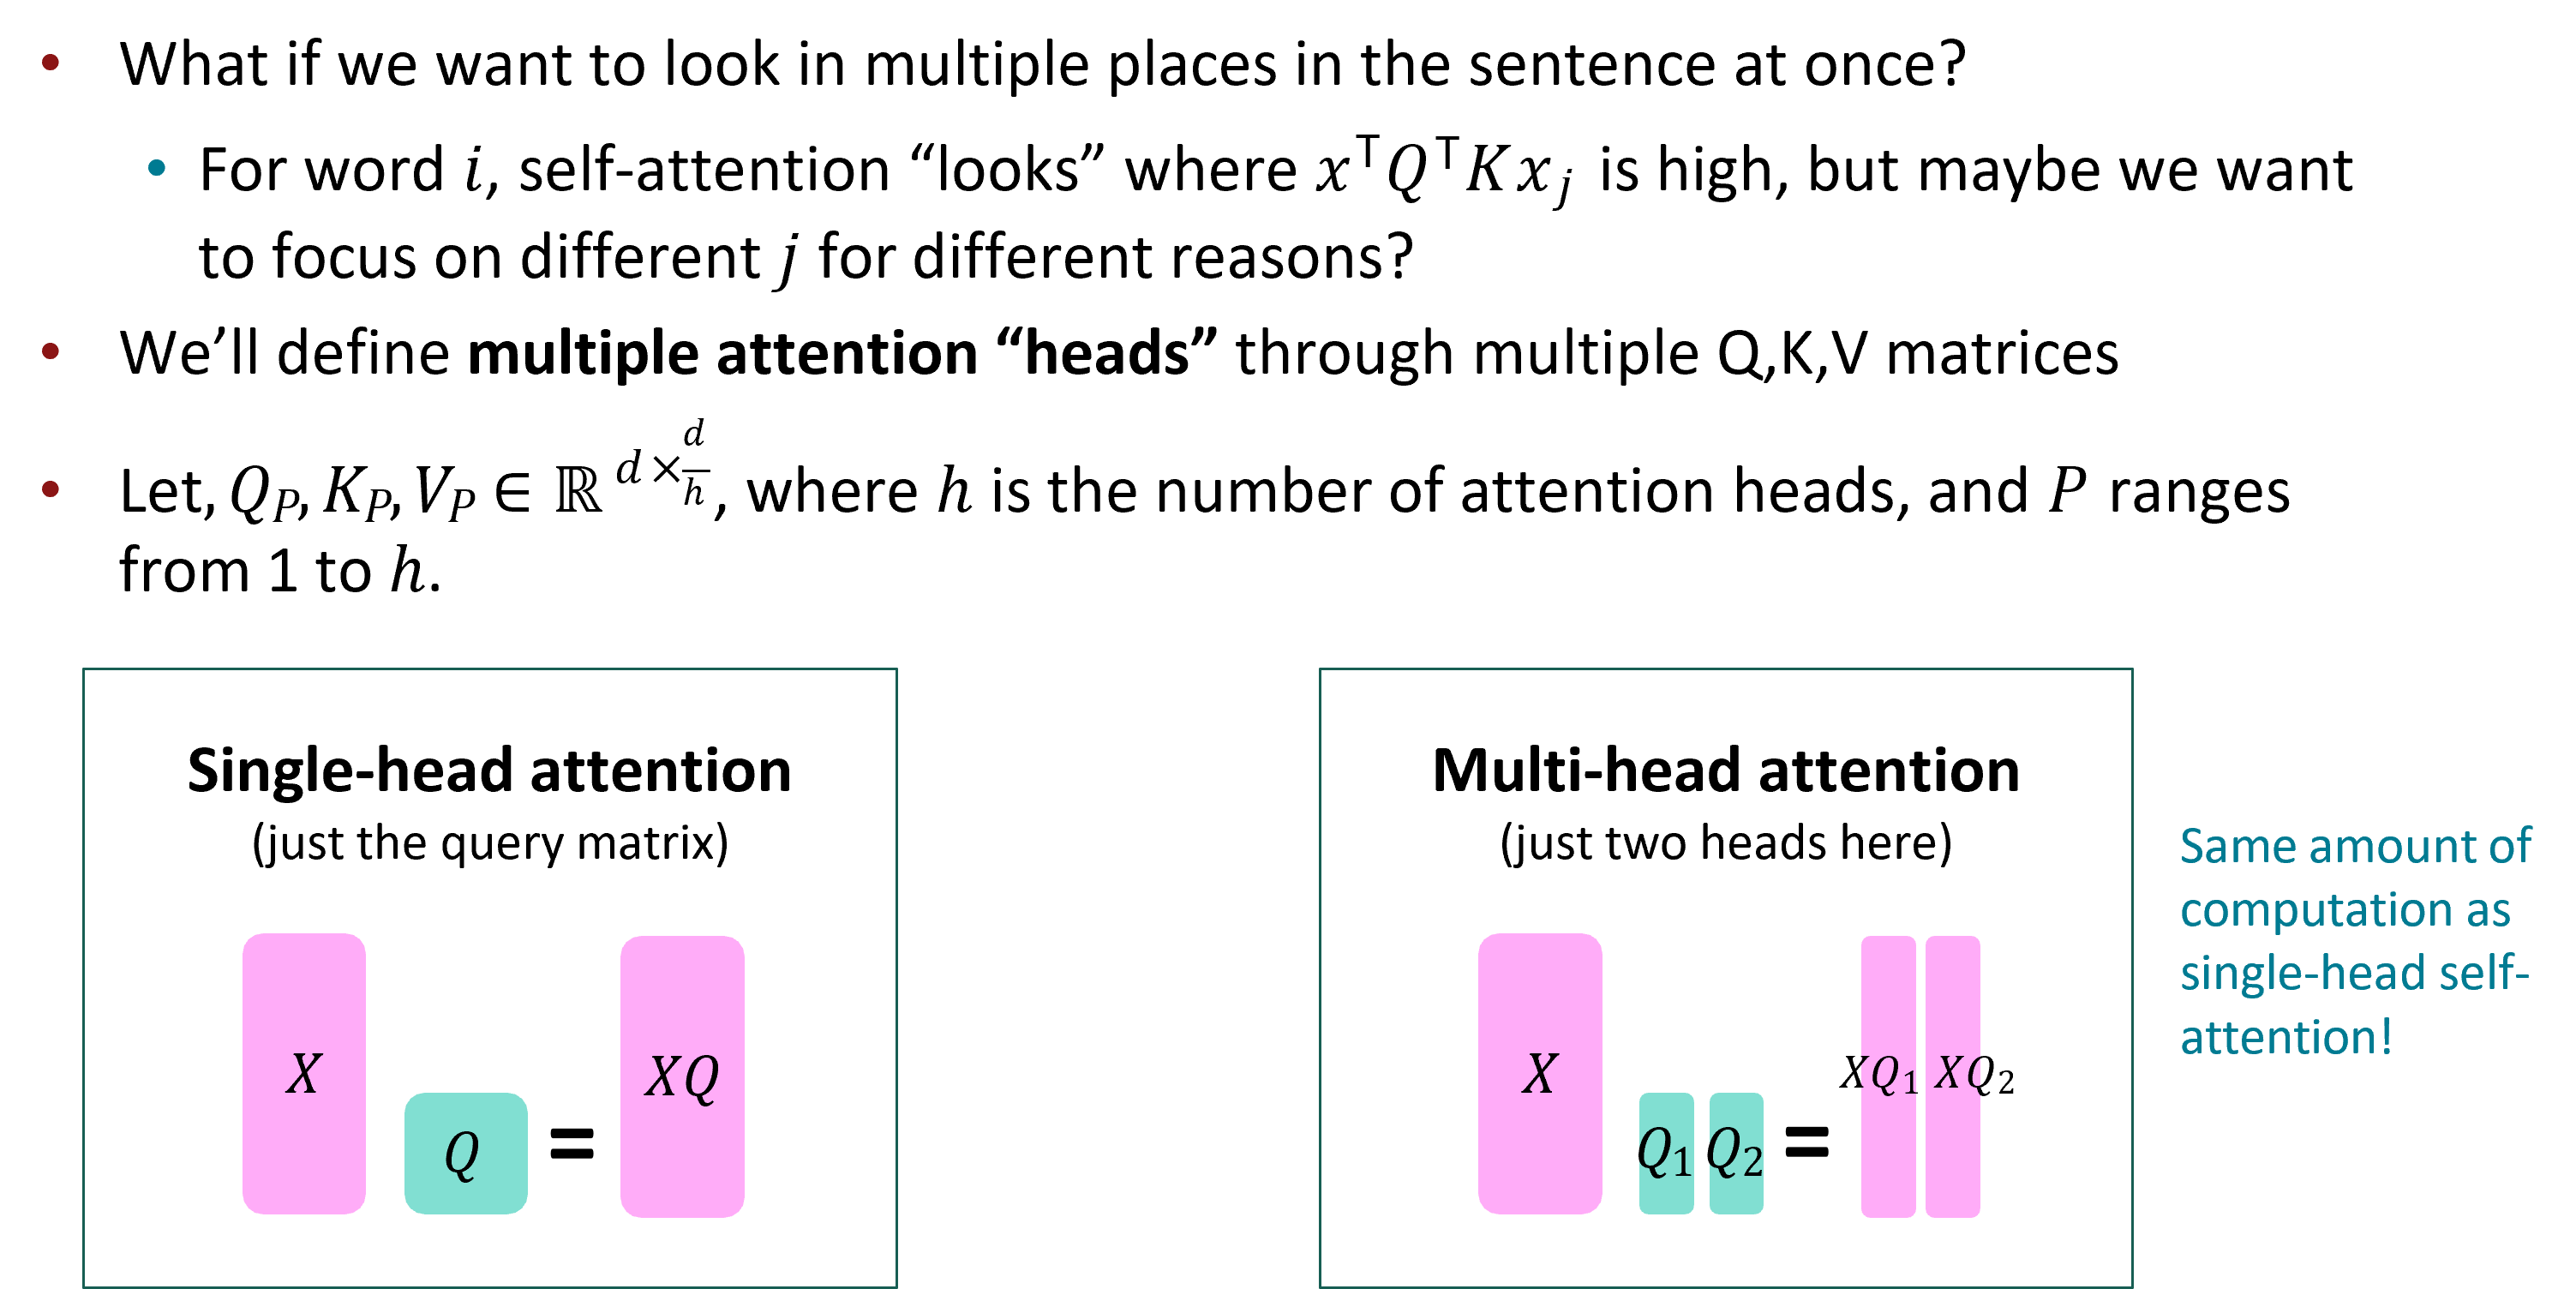
\includegraphics[width=\linewidth,keepaspectratio]{bert78}
			% \end{center}		
			
% % {\tiny (Ref: Language \& Machine Learning - John Hewitt)}

% \end{frame}

% %%%%%%%%%%%%%%%%%%%%%%%%%%%%%%%%%%%%%%%%%%%%%%%%%%%%%%%%%%%
% \begin{frame}[fragile]\frametitle{Attention visualization in layer 5}

			
			% \begin{center}
			% 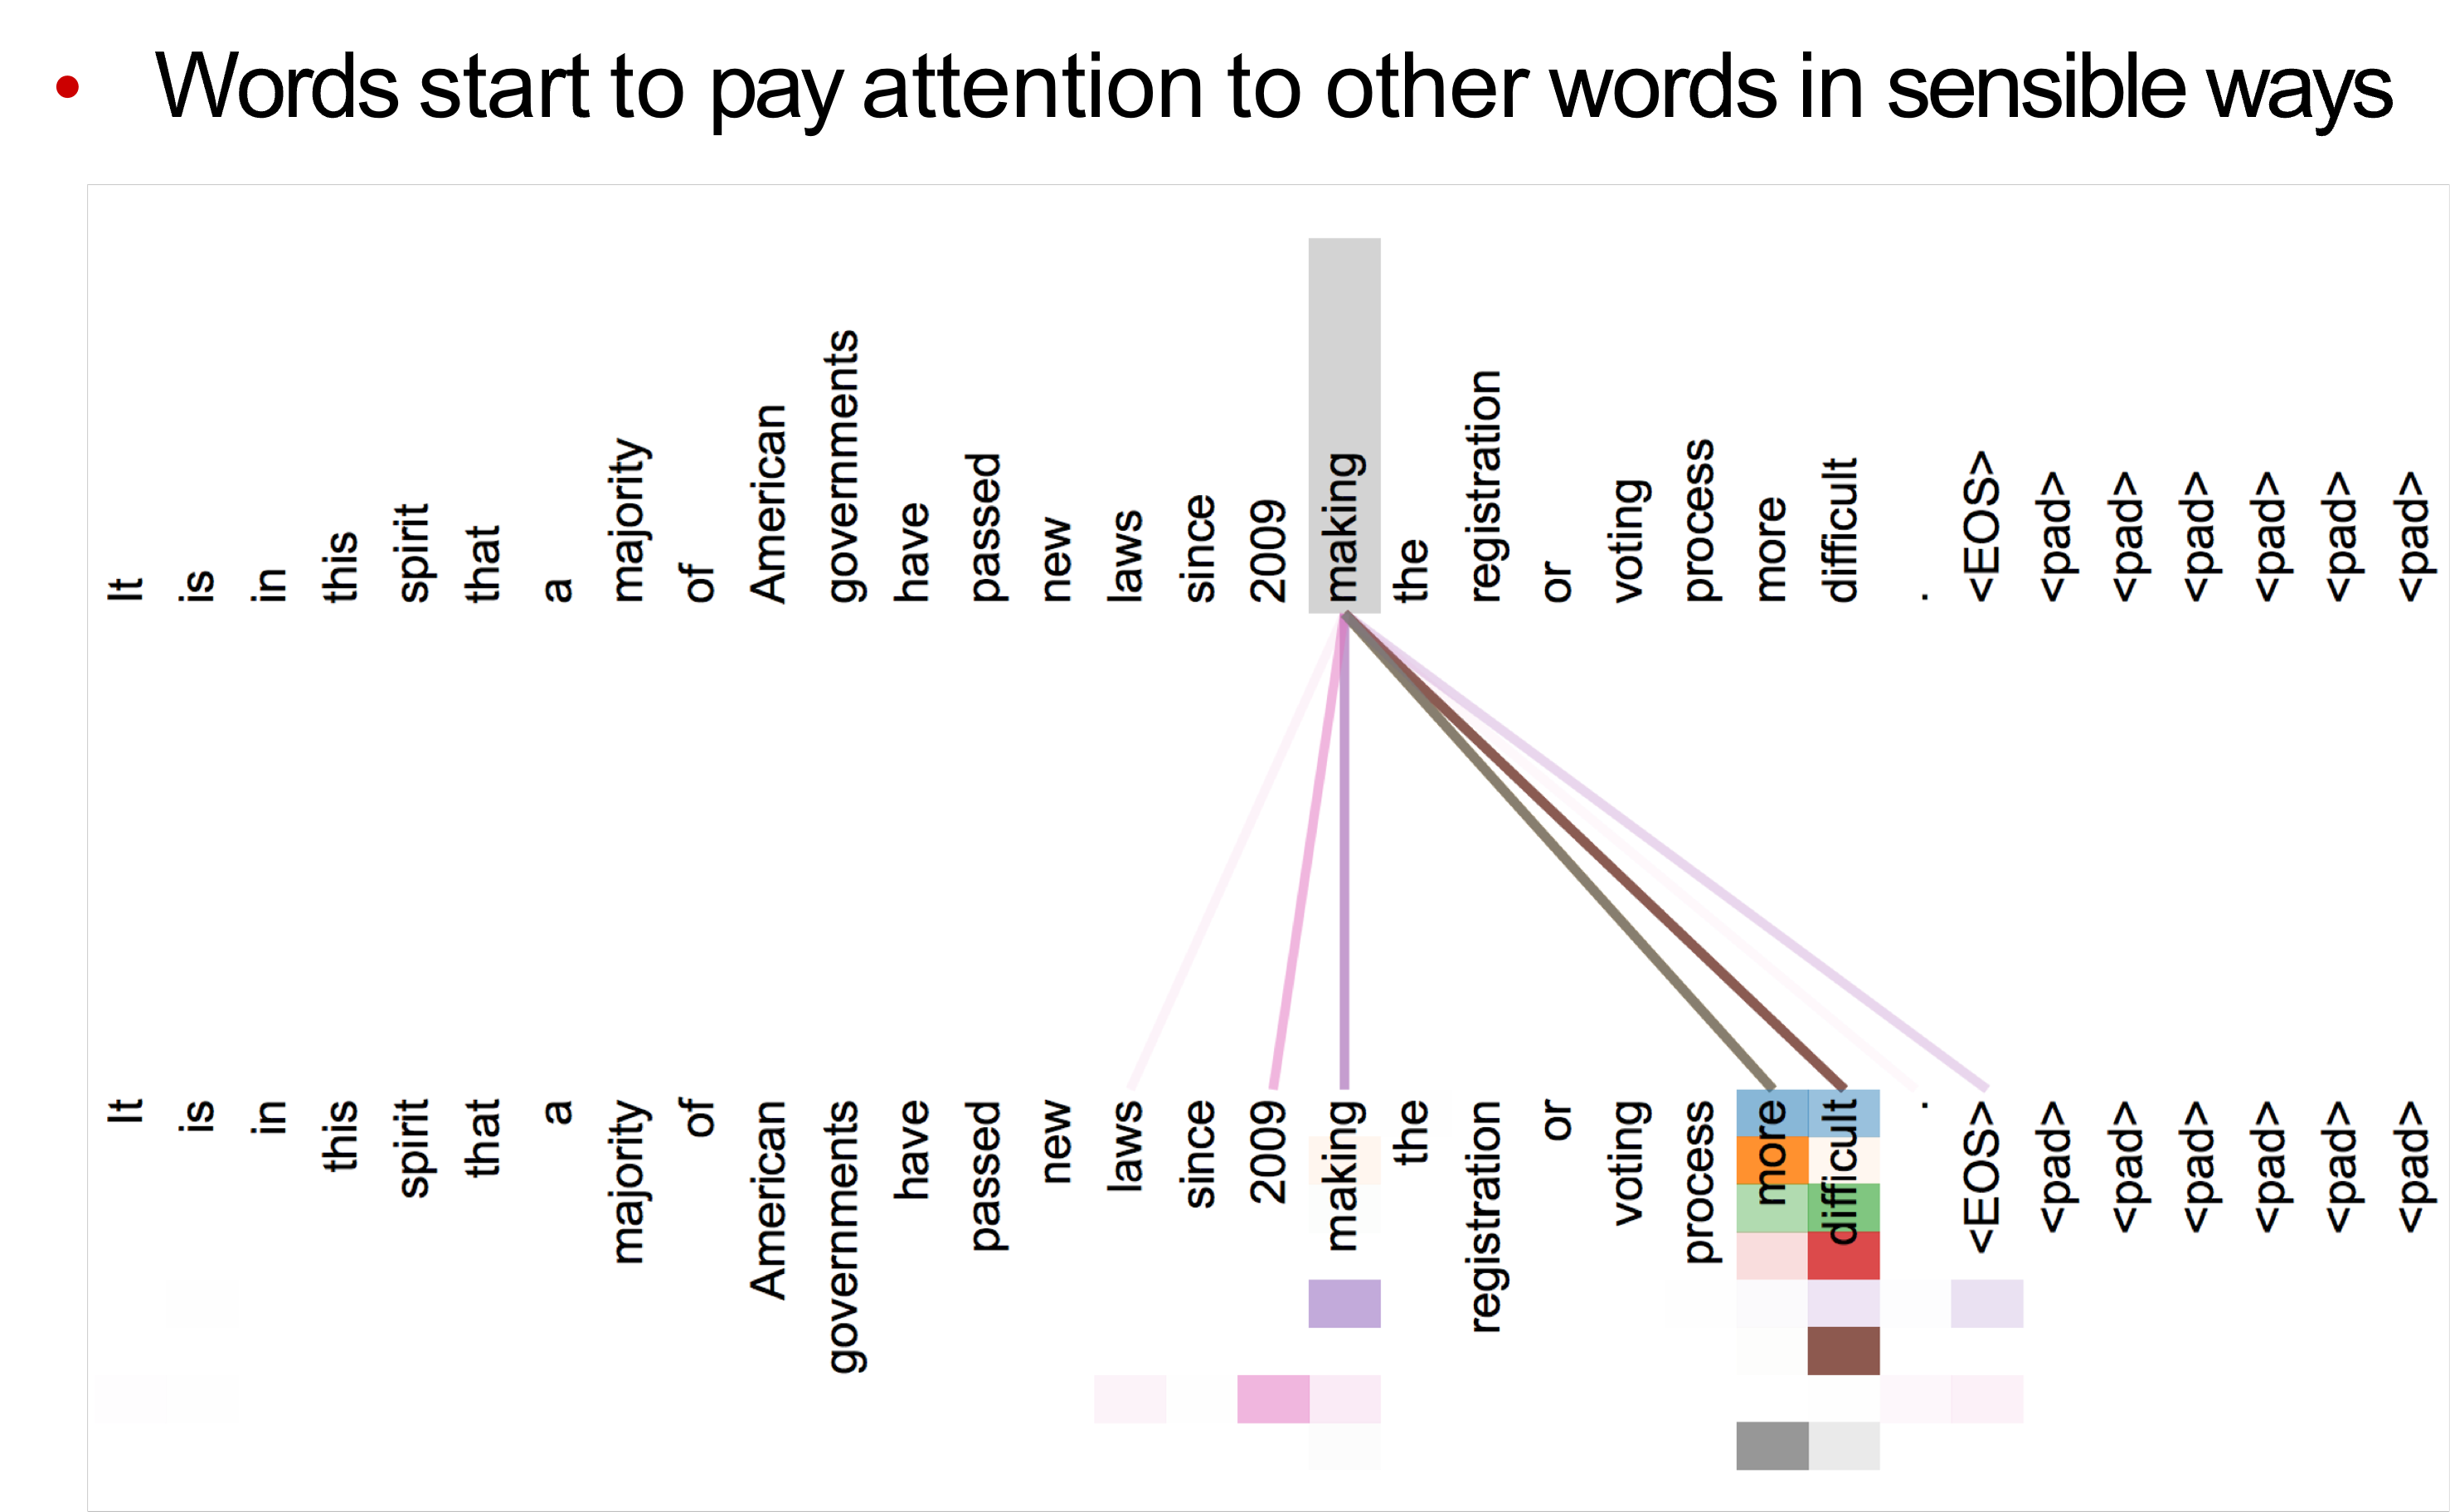
\includegraphics[width=0.8\linewidth,keepaspectratio]{bert79}
			% \end{center}		
			
			% % {\tiny (Ref: CS224n: Natural Language Processing with Deep Learning - Christopher Manning)}

% \end{frame}

% %%%%%%%%%%%%%%%%%%%%%%%%%%%%%%%%%%%%%%%%%%%%%%%%%%%%%%%%%%%
% \begin{frame}[fragile]\frametitle{Attention visualization: Implicit anaphora resolution}

			
			% \begin{center}
			% 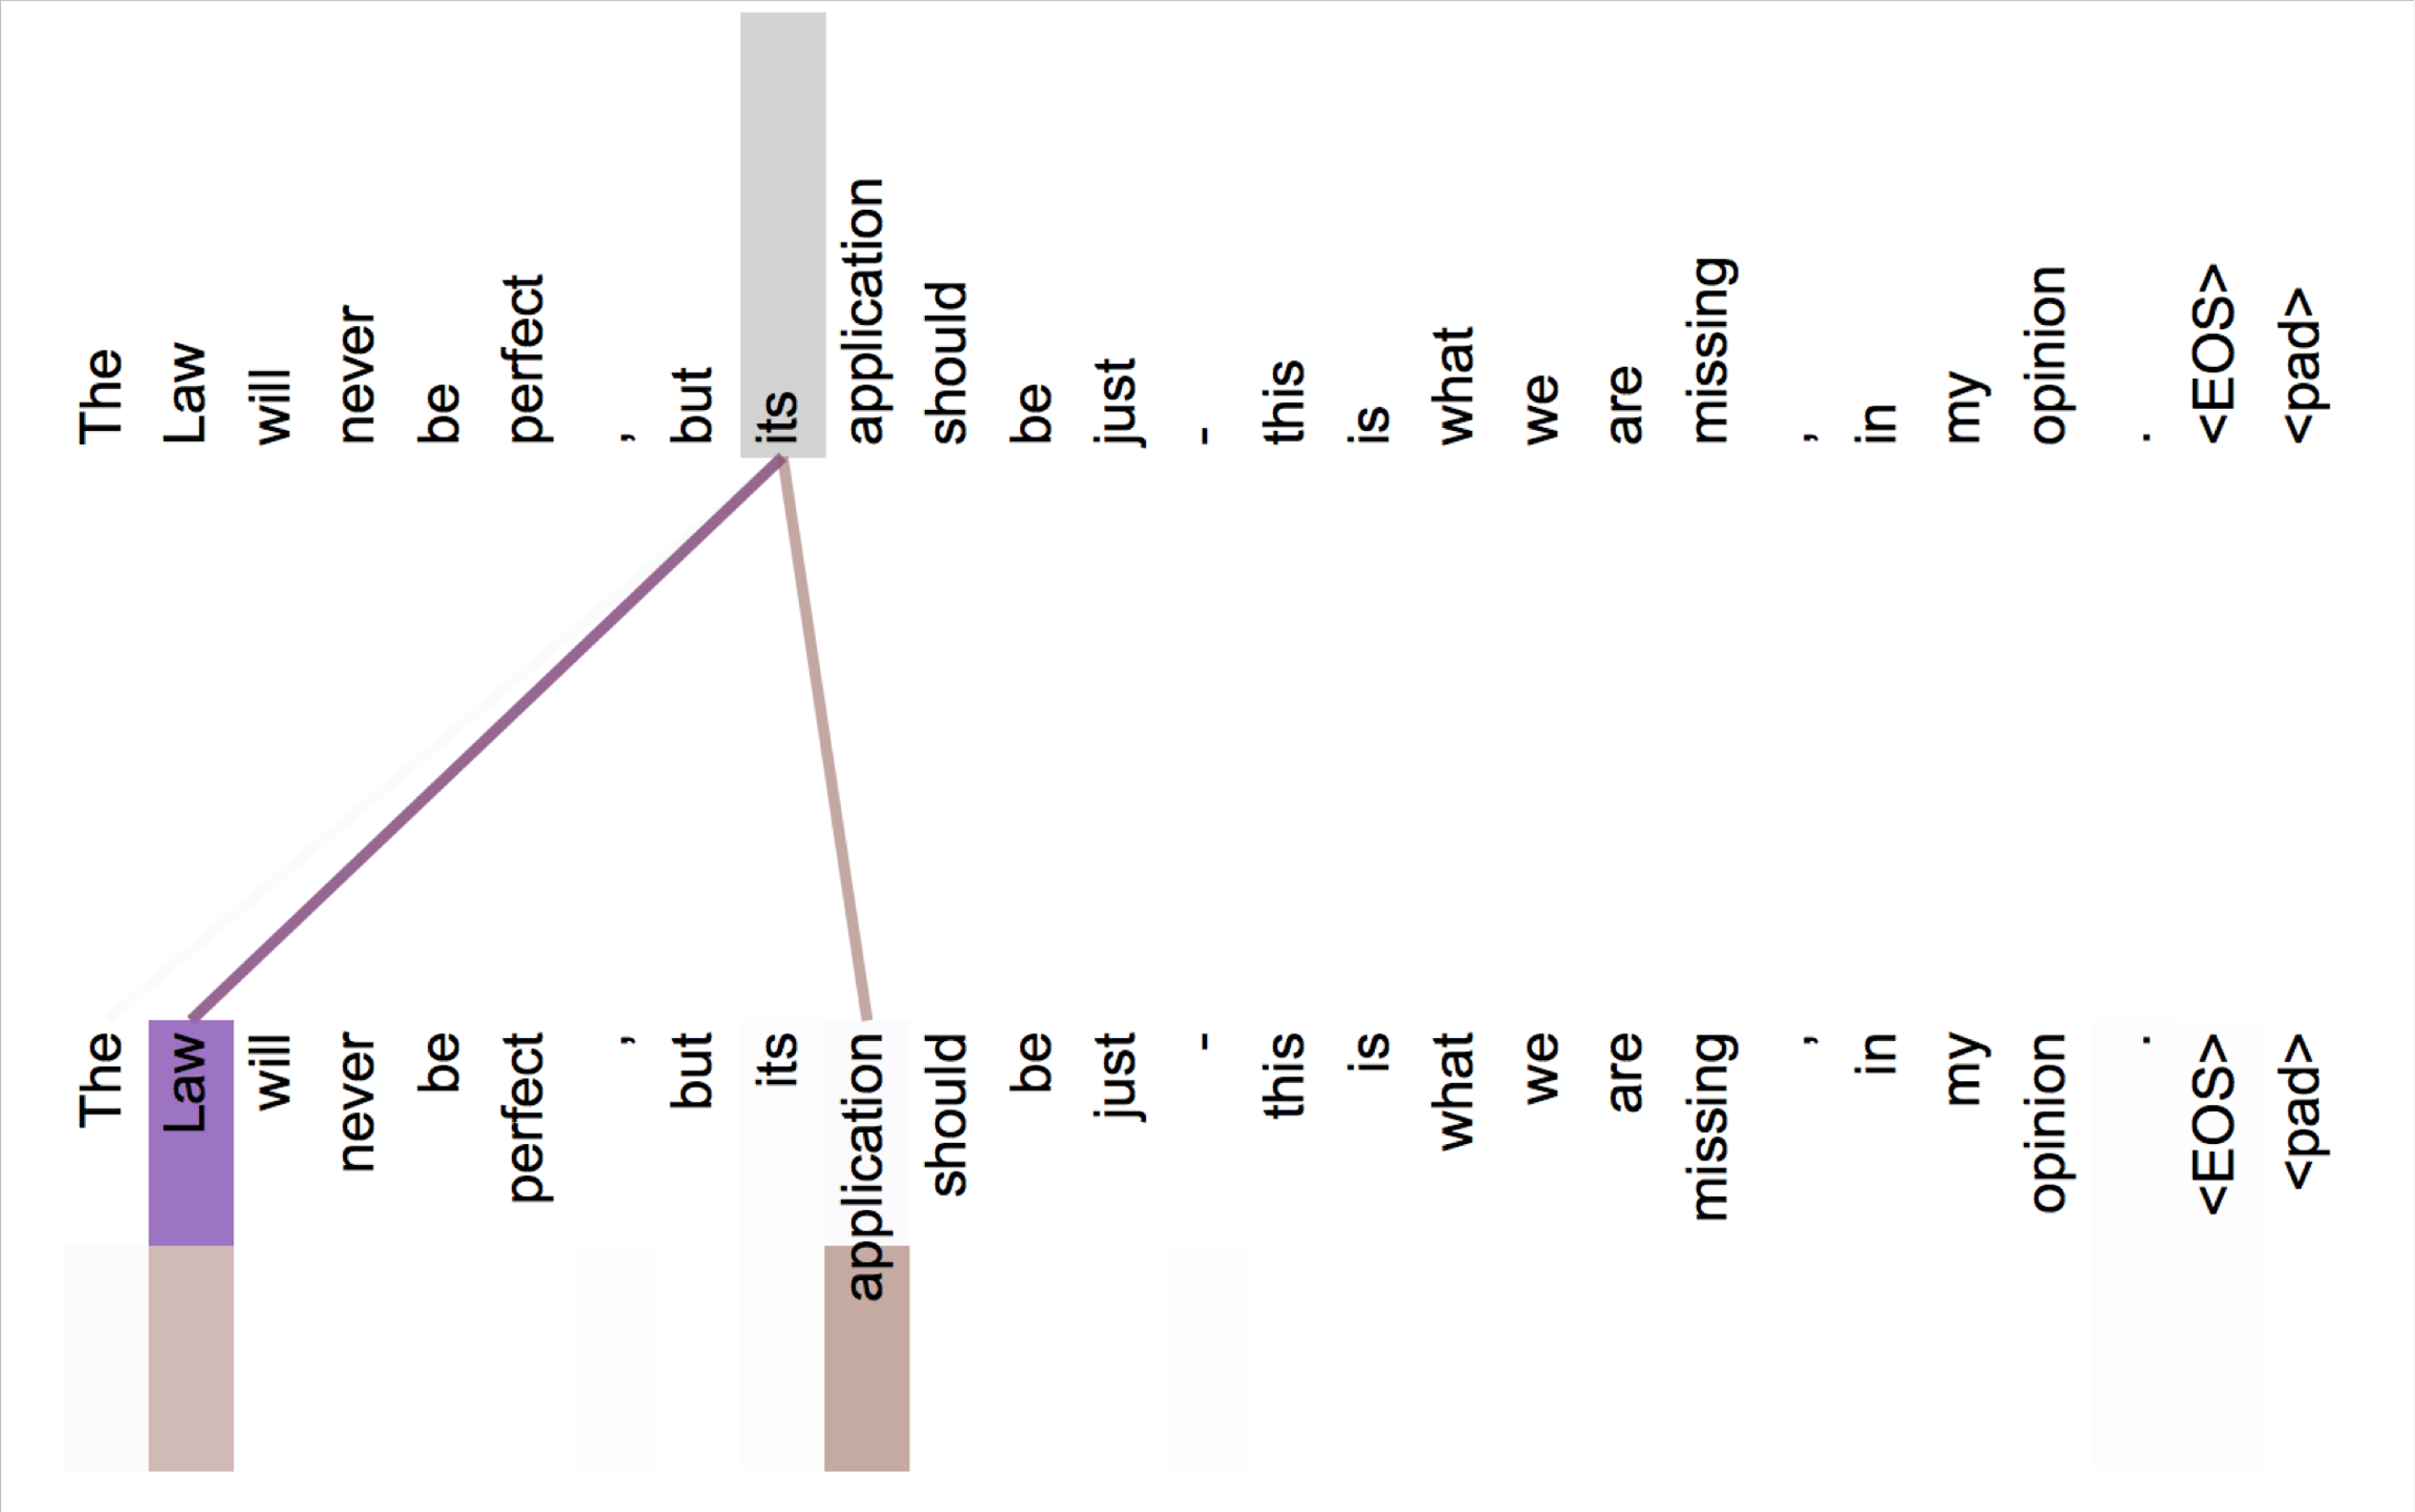
\includegraphics[width=0.6\linewidth,keepaspectratio]{bert80}
			% \end{center}		
			
			% In 5th layer. Isolated attentions from just the word ‘its’ for attention heads 5 and 6.  Note that the attentions are very sharp for this word.

			
			% % {\tiny (Ref: CS224n: Natural Language Processing with Deep Learning - Christopher Manning)}

% \end{frame}

% %%%%%%%%%%%%%%%%%%%%%%%%%%%%%%%%%%%%%%%%%%%%%%%%%%%%%%%%%%%
% \begin{frame}[fragile]\frametitle{Parallel attention heads}

			
			% \begin{center}
			% 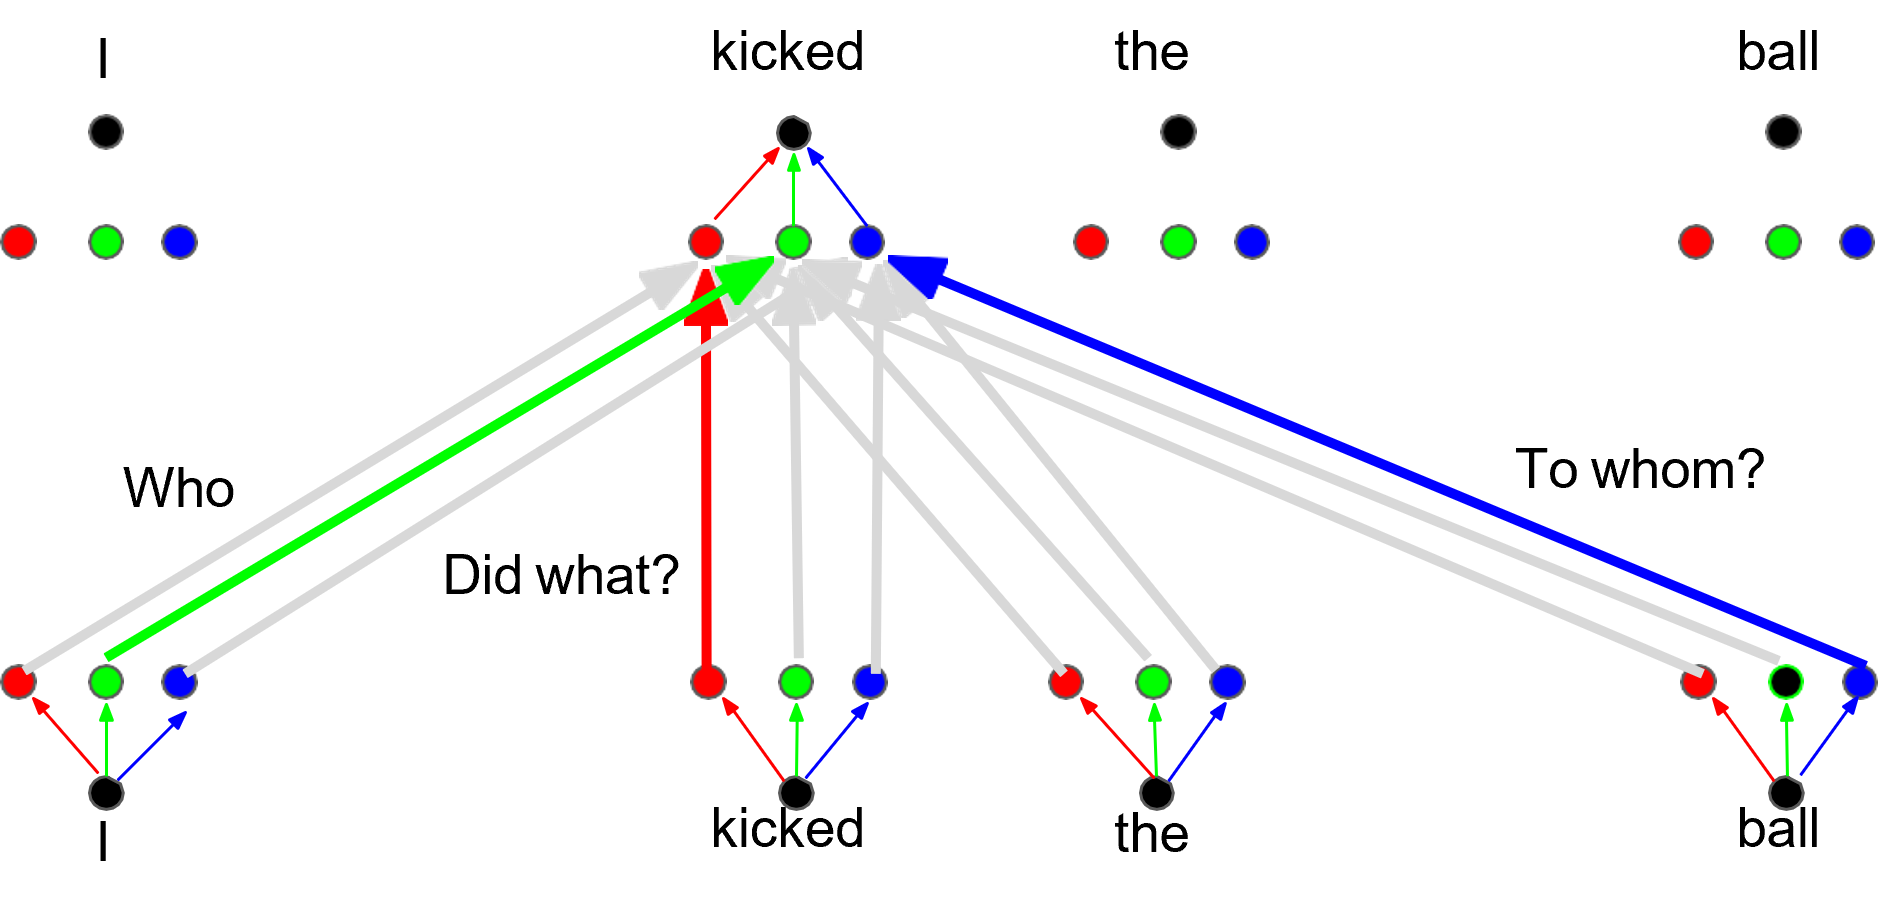
\includegraphics[width=0.6\linewidth,keepaspectratio]{bert81}
			% \end{center}		
			
		
			% % {\tiny (Ref: Ashish Vaswani)}

% \end{frame}

%%%%%%%%%%%%%%%%%%%%%%%%%%%%%%%%%%%%%%%%%%%%%%%%%%%%%%%%%%%%%%%%%%%%%%%%%%%%%%%%%%
\begin{frame}[fragile]\frametitle{}
\begin{center}
{\Large Feed Forward}
\end{center}
\end{frame}

%%%%%%%%%%%%%%%%%%%%%%%%%%%%%%%%%%%%%%%%%%%%%%%%%%%%%%%%%%%
\begin{frame}[fragile]\frametitle{Feed Forward}

\begin{itemize}
\item The feed-forward layer operates on the output of the multi-headed self-attention layer.
\item It treats each position of the global representation independently.
\item It does not take the relationship between elements into consideration.
\item The feed-forward layers contain weights that are tuned during training.
\item There are two linear transformations/layers ($W_1,W_2$) with a non-linear activation function (usually ReLU) in between. 
\item This non-linearity allows the model to capture complex relationships in data, relationships which aren’t directly related.
\item The result of the feed-forward layer is added back to the global\_representation matrix through a residual connection
\item Note that  that this operation is addition, rather than concatenation. This means that residual\_output is the global\_representation matrix enhanced by the knowledge gleaned from the feed-forward neural network.
\item residual\_output is normalised. This step is necessary to reduce internal covariate shift and stabilise training. To put it simply, if internal parameters change too rapidly between each layer the model cannot learn properly.
\end{itemize}


{\tiny (Ref: Unlocking the Transformer: Advancing Technology From RNNs and LSTMs - Anthony Gavriel)}


\begin{lstlisting}
FNN_output_1 = ReLU((i_output * W1 + b1)) * W2 + b2
FNN_output_2 = ReLU((love_output * W1 + b1)) * W2 + b2
FNN_output_3 = ReLU((cats_output * W1 + b1)) * W2 + b2

residual_output = global_representation + FNN_output_1 + FNN_output_2 + FNN_output_3

\end{lstlisting}

\end{frame}



%%%%%%%%%%%%%%%%%%%%%%%%%%%%%%%%%%%%%%%%%%%%%%%%%%%%%%%%%%%%%%%%%%%%%%%%%%%%%%%%%%
\begin{frame}[fragile]\frametitle{}
\begin{center}
{\Large Add \& Norm}
\end{center}
\end{frame}

%%%%%%%%%%%%%%%%%%%%%%%%%%%%%%%%%%%%%%%%%%%%%%%%%%%%%%%%%%%
\begin{frame}[fragile]\frametitle{The Residuals}


\begin{center}
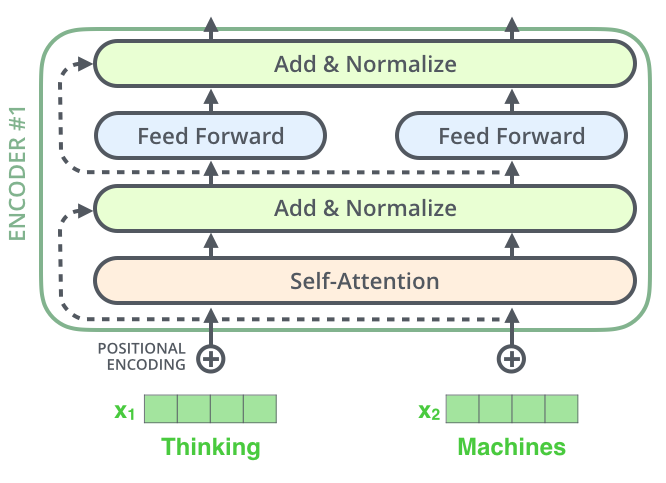
\includegraphics[width=0.6\linewidth,keepaspectratio]{transformer_resideual_layer_norm_jay}


{\tiny (Ref: ``The Illustrated Transformer'' - Jay Alammar)}
\end{center}		

Each sub-layer (self-attention, ffnn) in each encoder has a residual connection around it, and is followed by a layer-normalization step.

The dotted line means, sometimes, the self-attention block wont be considered/skipped and directed next Add/Normalize block is taken up.

\end{frame}

%%%%%%%%%%%%%%%%%%%%%%%%%%%%%%%%%%%%%%%%%%%%%%%%%%%%%%%%%%%
\begin{frame}[fragile]\frametitle{Visualize The Residuals}

Visualize the vectors and the layer-norm operation associated with self attention, it would look like this:

\begin{center}
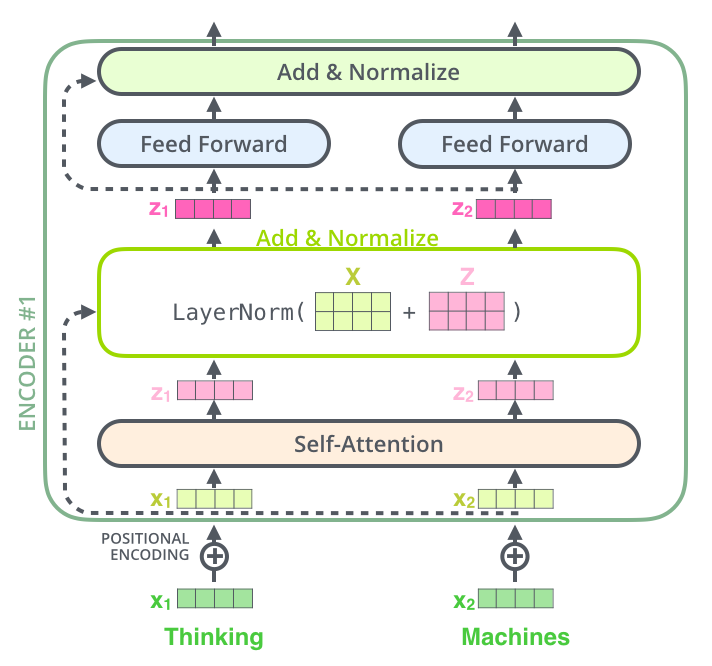
\includegraphics[width=0.6\linewidth,keepaspectratio]{transformer_resideual_layer_norm_2_jay}


{\tiny (Ref: ``The Illustrated Transformer'' - Jay Alammar)}
\end{center}		

\end{frame}

%%%%%%%%%%%%%%%%%%%%%%%%%%%%%%%%%%%%%%%%%%%%%%%%%%%%%%%%%%%
\begin{frame}[fragile]\frametitle{Also for the Decoder}

\begin{center}
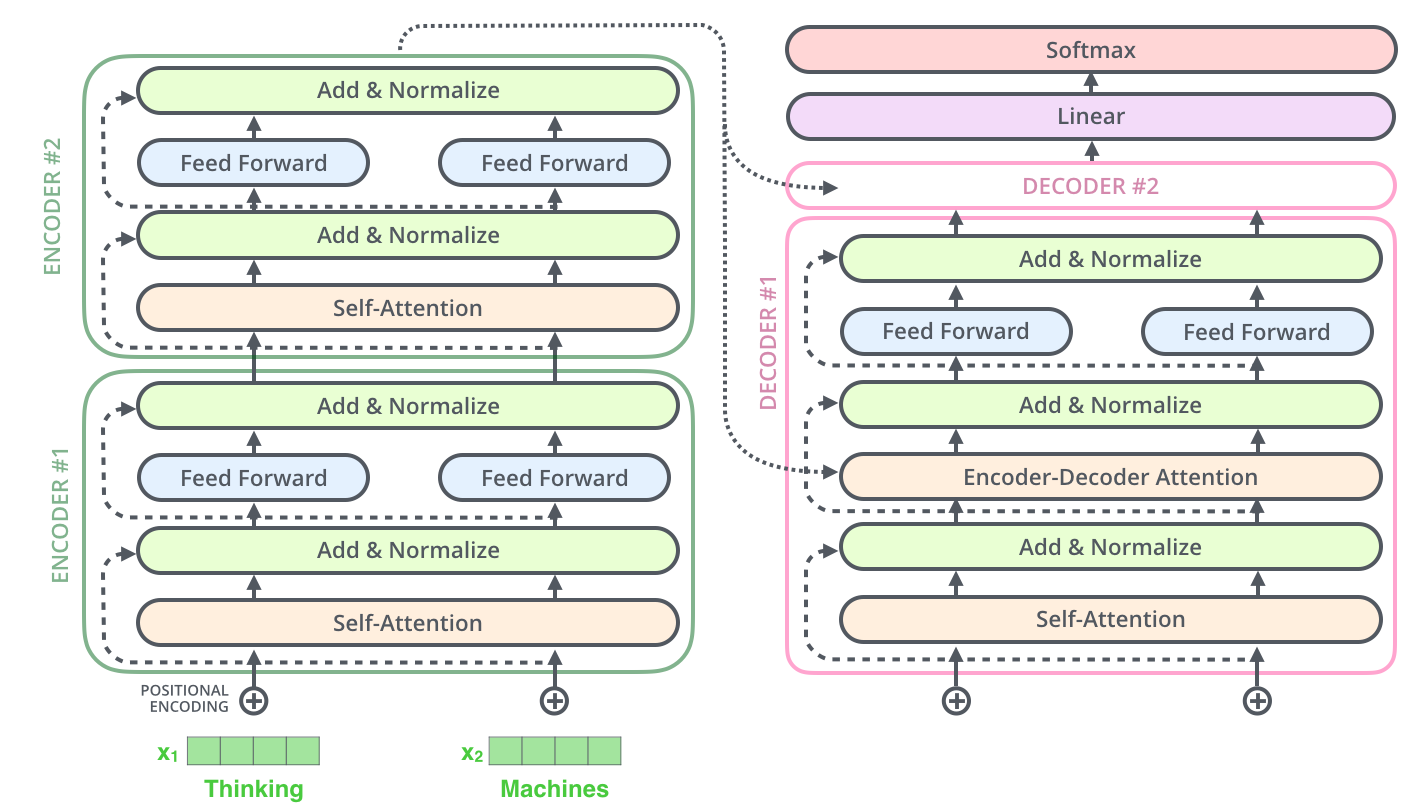
\includegraphics[width=\linewidth,keepaspectratio]{transformer_resideual_layer_norm_3_jay}


{\tiny (Ref: ``The Illustrated Transformer'' - Jay Alammar)}
\end{center}		

Output of Encoders ($K$ and $V$) are passed to 'Cross Attention' layers of each decoder cell.

\end{frame}


% %%%%%%%%%%%%%%%%%%%%%%%%%%%%%%%%%%%%%%%%%%%%%%%%%%%%%%%%%%%
% \begin{frame}[fragile]\frametitle{Residual connections}

			% The Transformer Encoder: Residual connections [He et al., 2016]
			
			% \begin{center}
			% 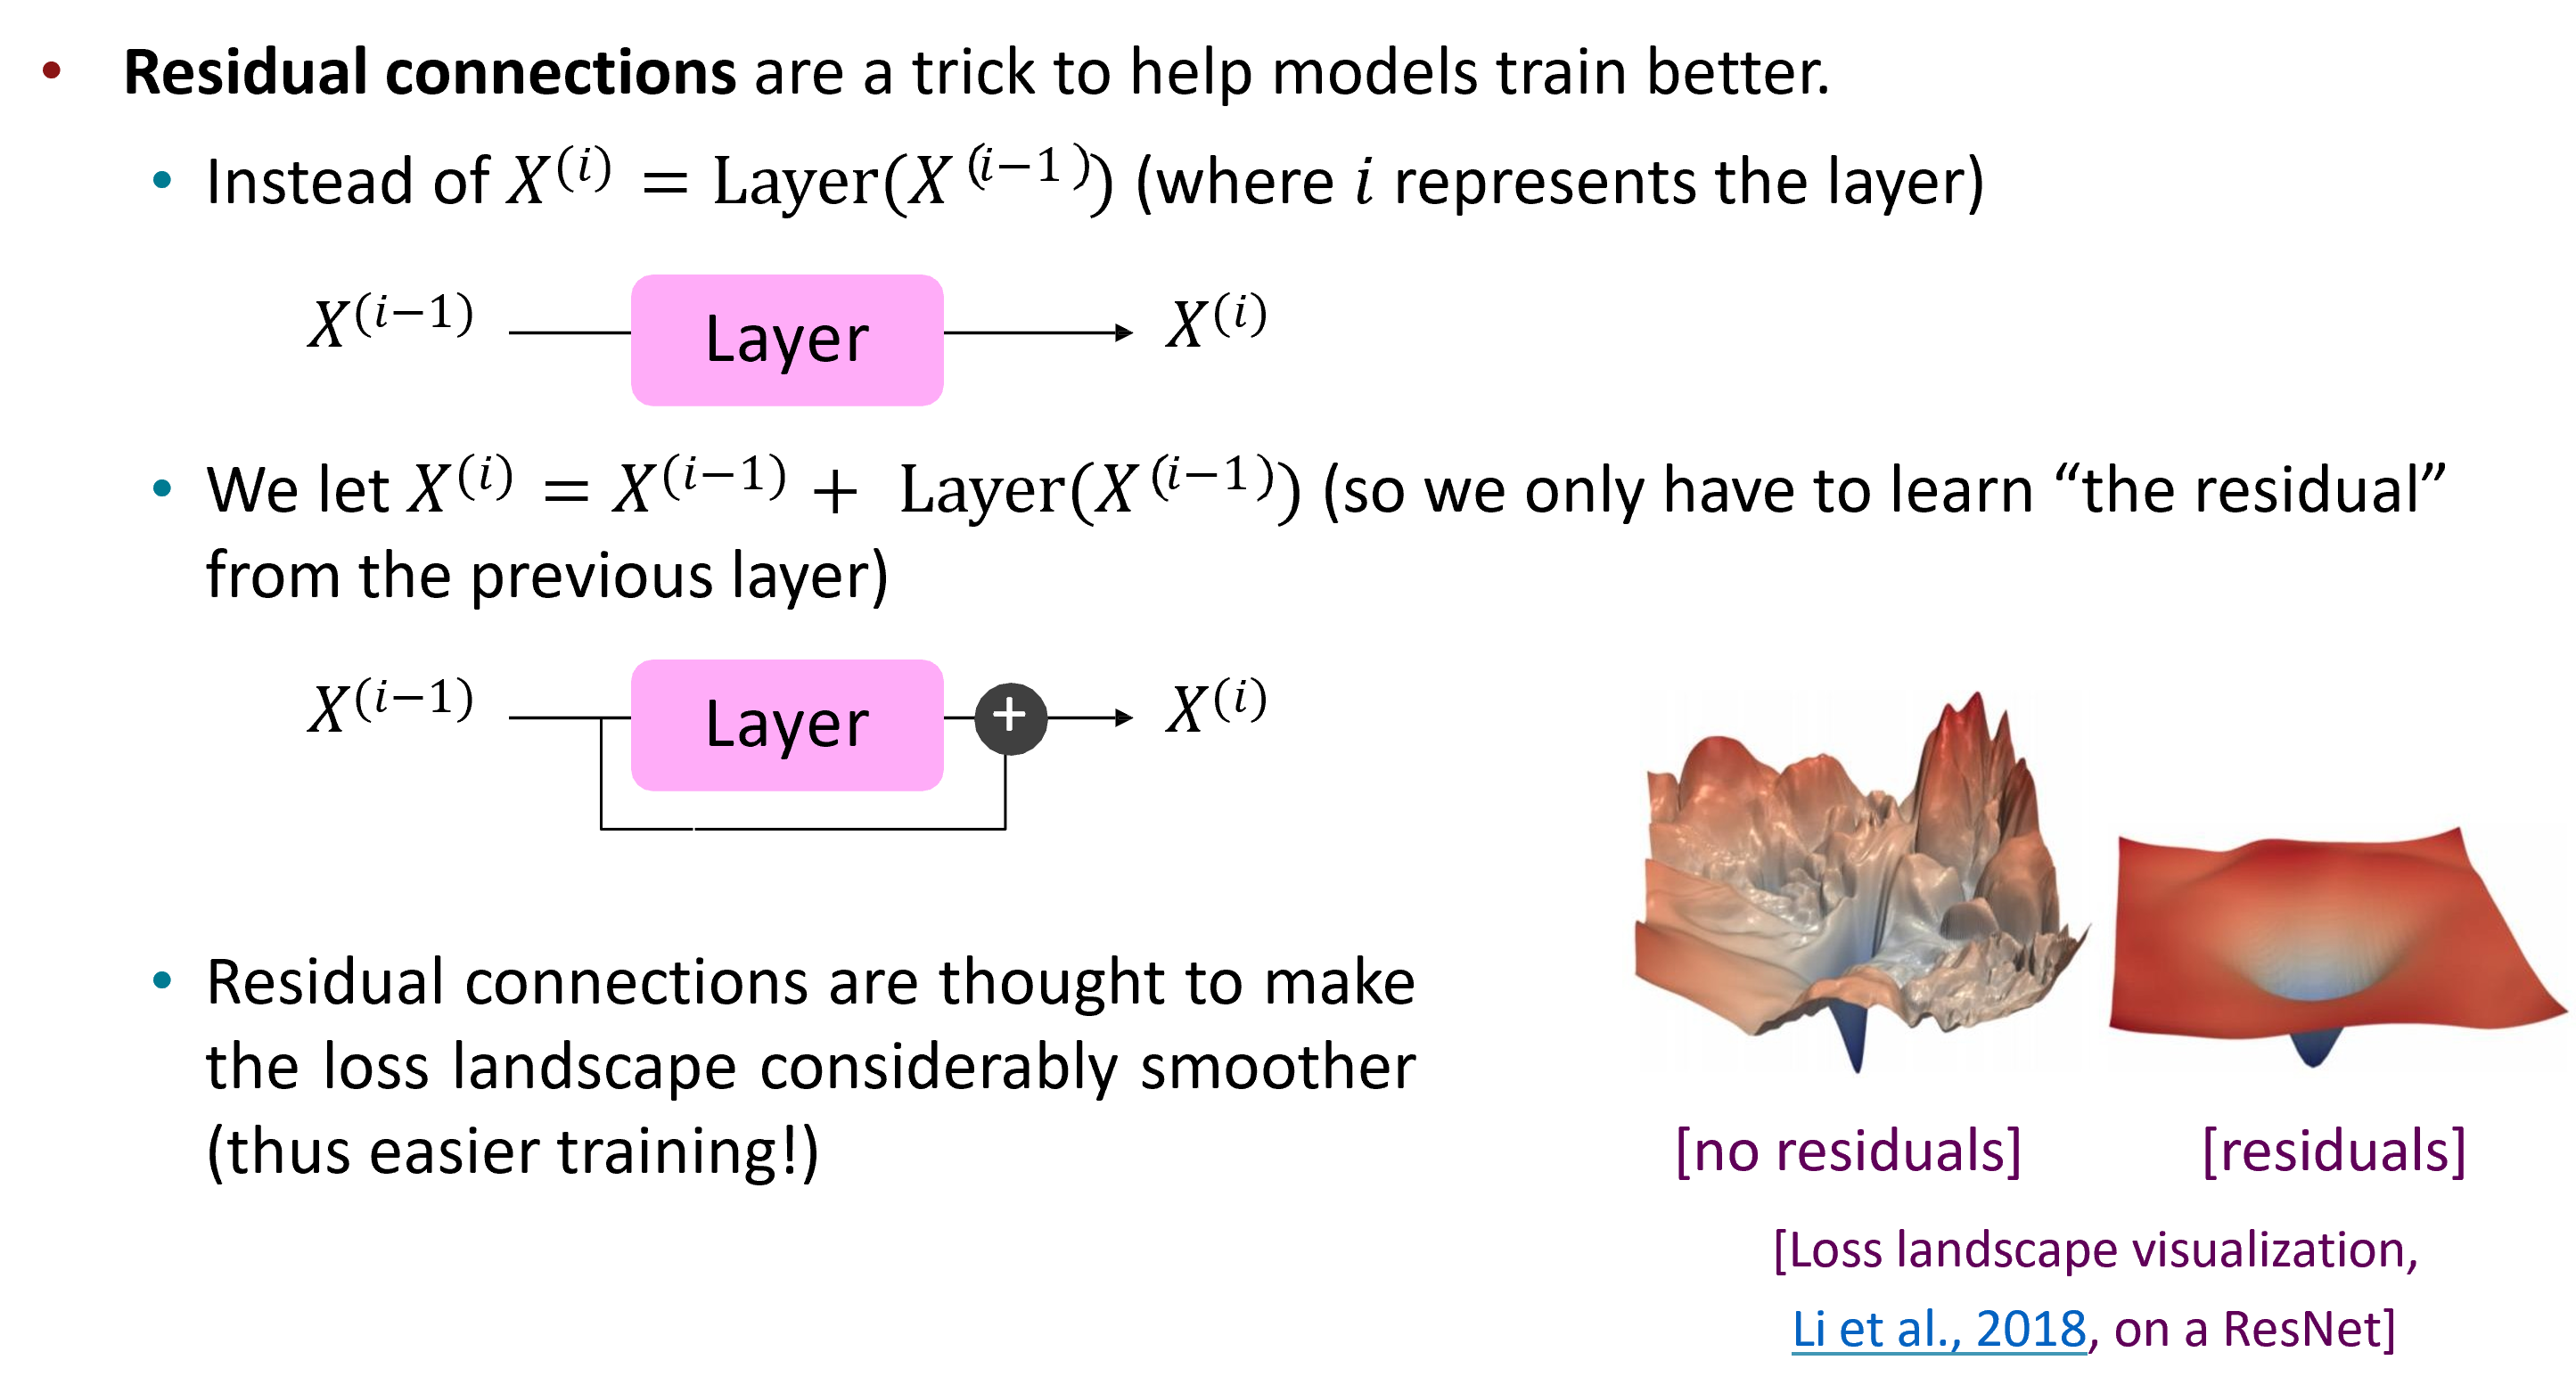
\includegraphics[width=\linewidth,keepaspectratio]{bert82}
			% \end{center}		
			
		
			% % {\tiny (Ref: John Hewitt)}

% \end{frame}

% %%%%%%%%%%%%%%%%%%%%%%%%%%%%%%%%%%%%%%%%%%%%%%%%%%%%%%%%%%%
% \begin{frame}[fragile]\frametitle{Layer normalization}
% The Transformer Encoder: Layer normalization [Ba et al., 2016]
			
			% \begin{center}
			% 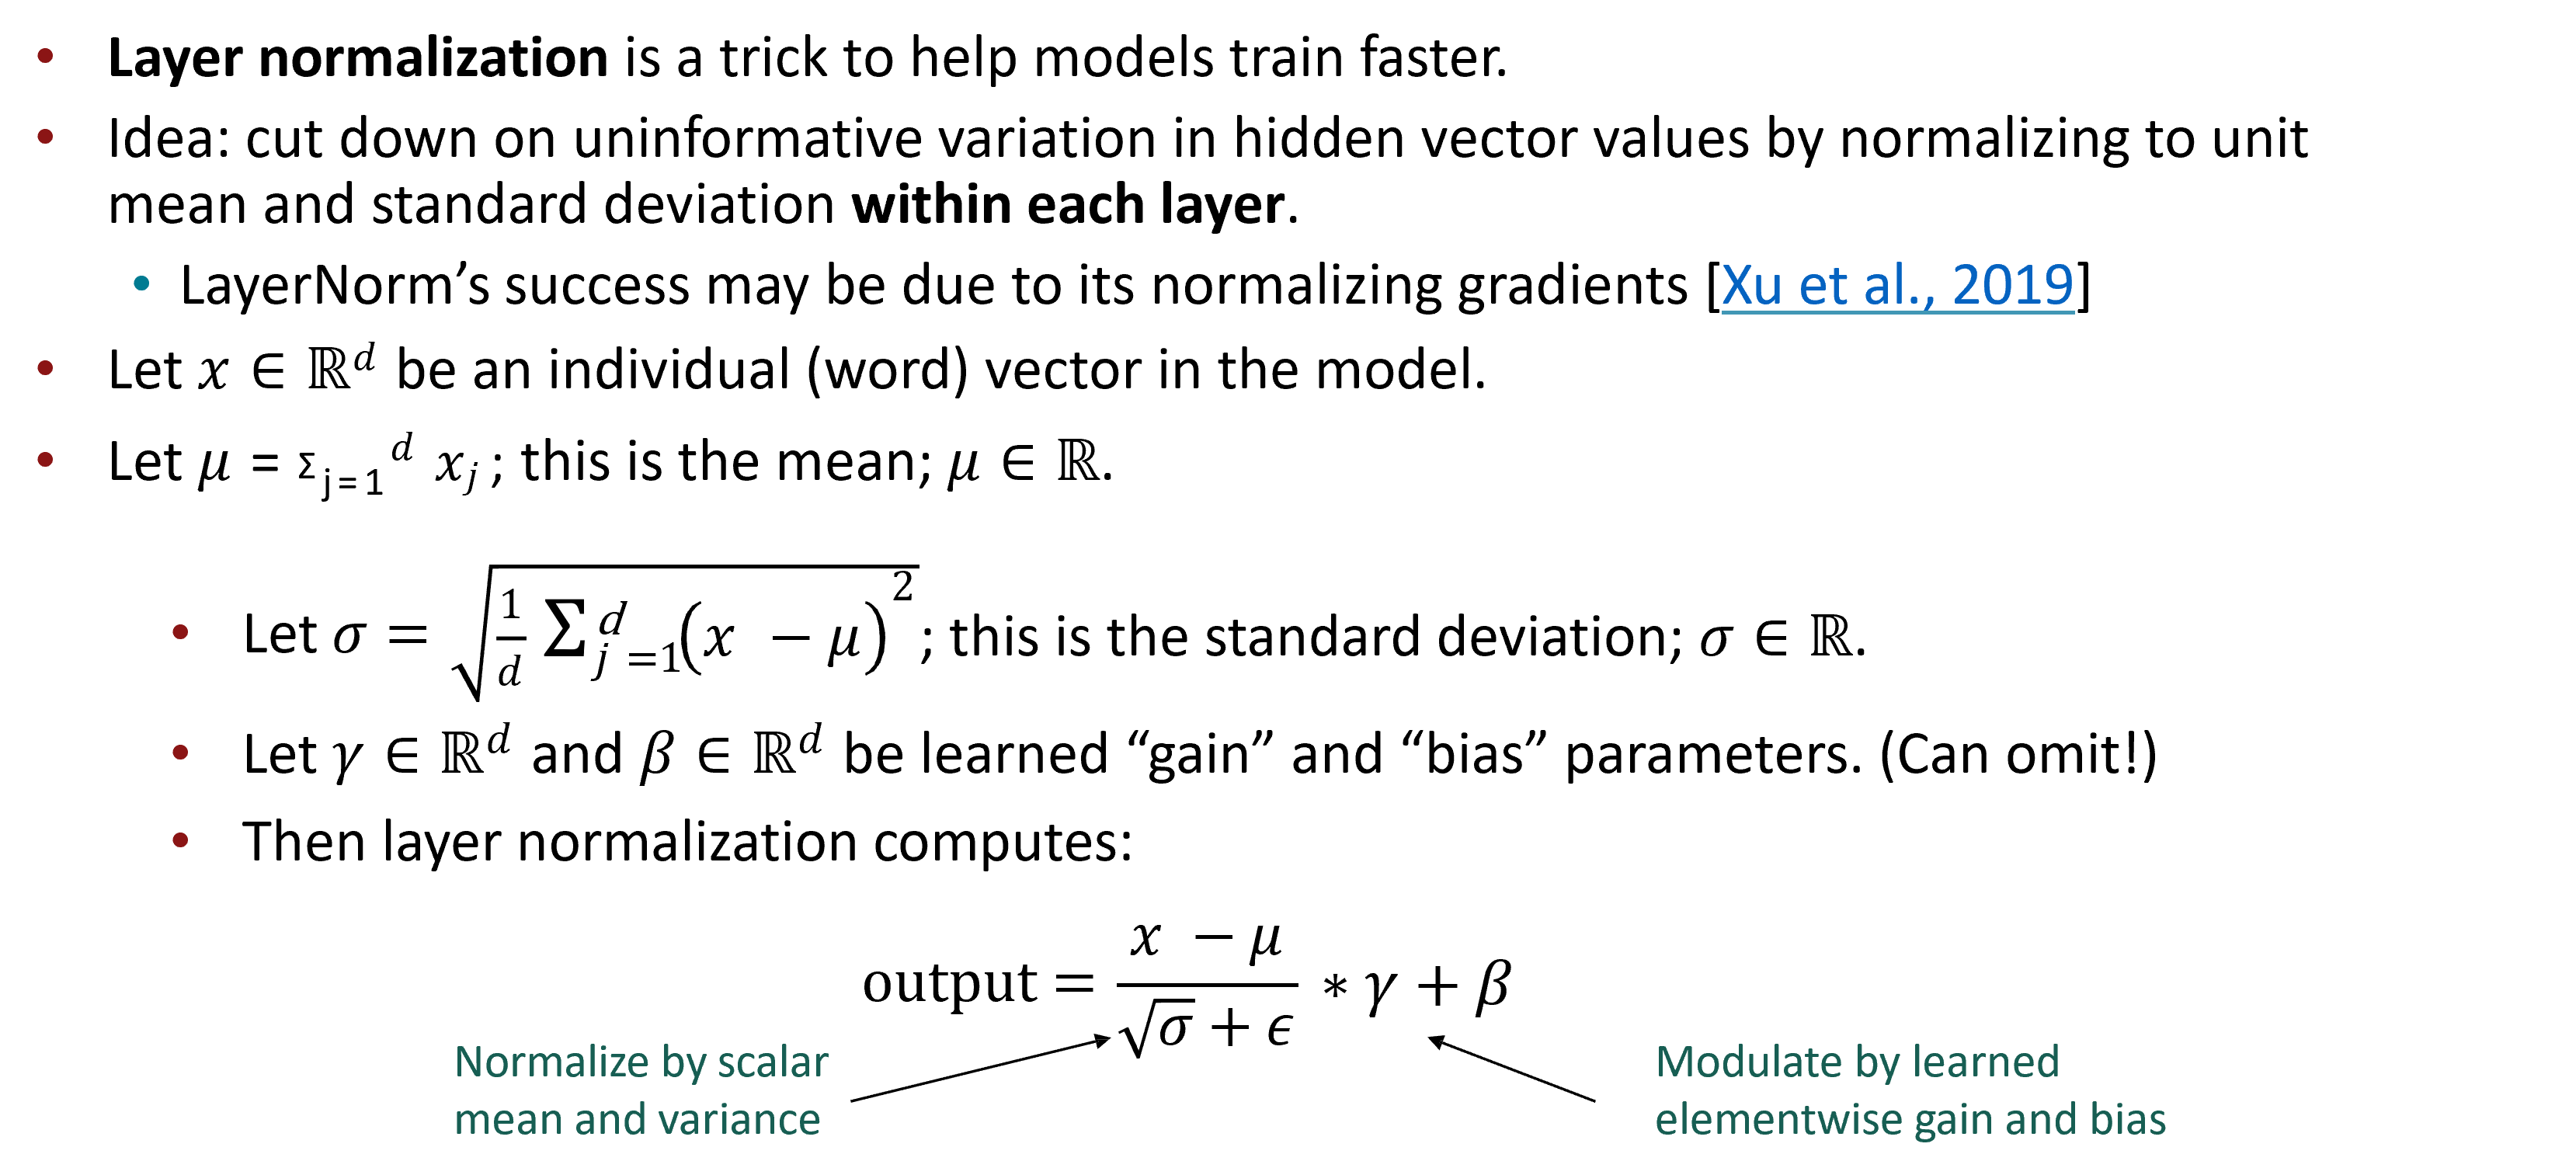
\includegraphics[width=\linewidth,keepaspectratio]{bert83}
			% \end{center}		
			
		
			% % {\tiny (Ref: John Hewitt)}

% \end{frame}

% %%%%%%%%%%%%%%%%%%%%%%%%%%%%%%%%%%%%%%%%%%%%%%%%%%%%%%%%%%%
% \begin{frame}[fragile]\frametitle{ Softmax}

			% The Transformer Encoder: Scaled Dot Product [Vaswani et al., 2017]
			% \begin{center}
			% 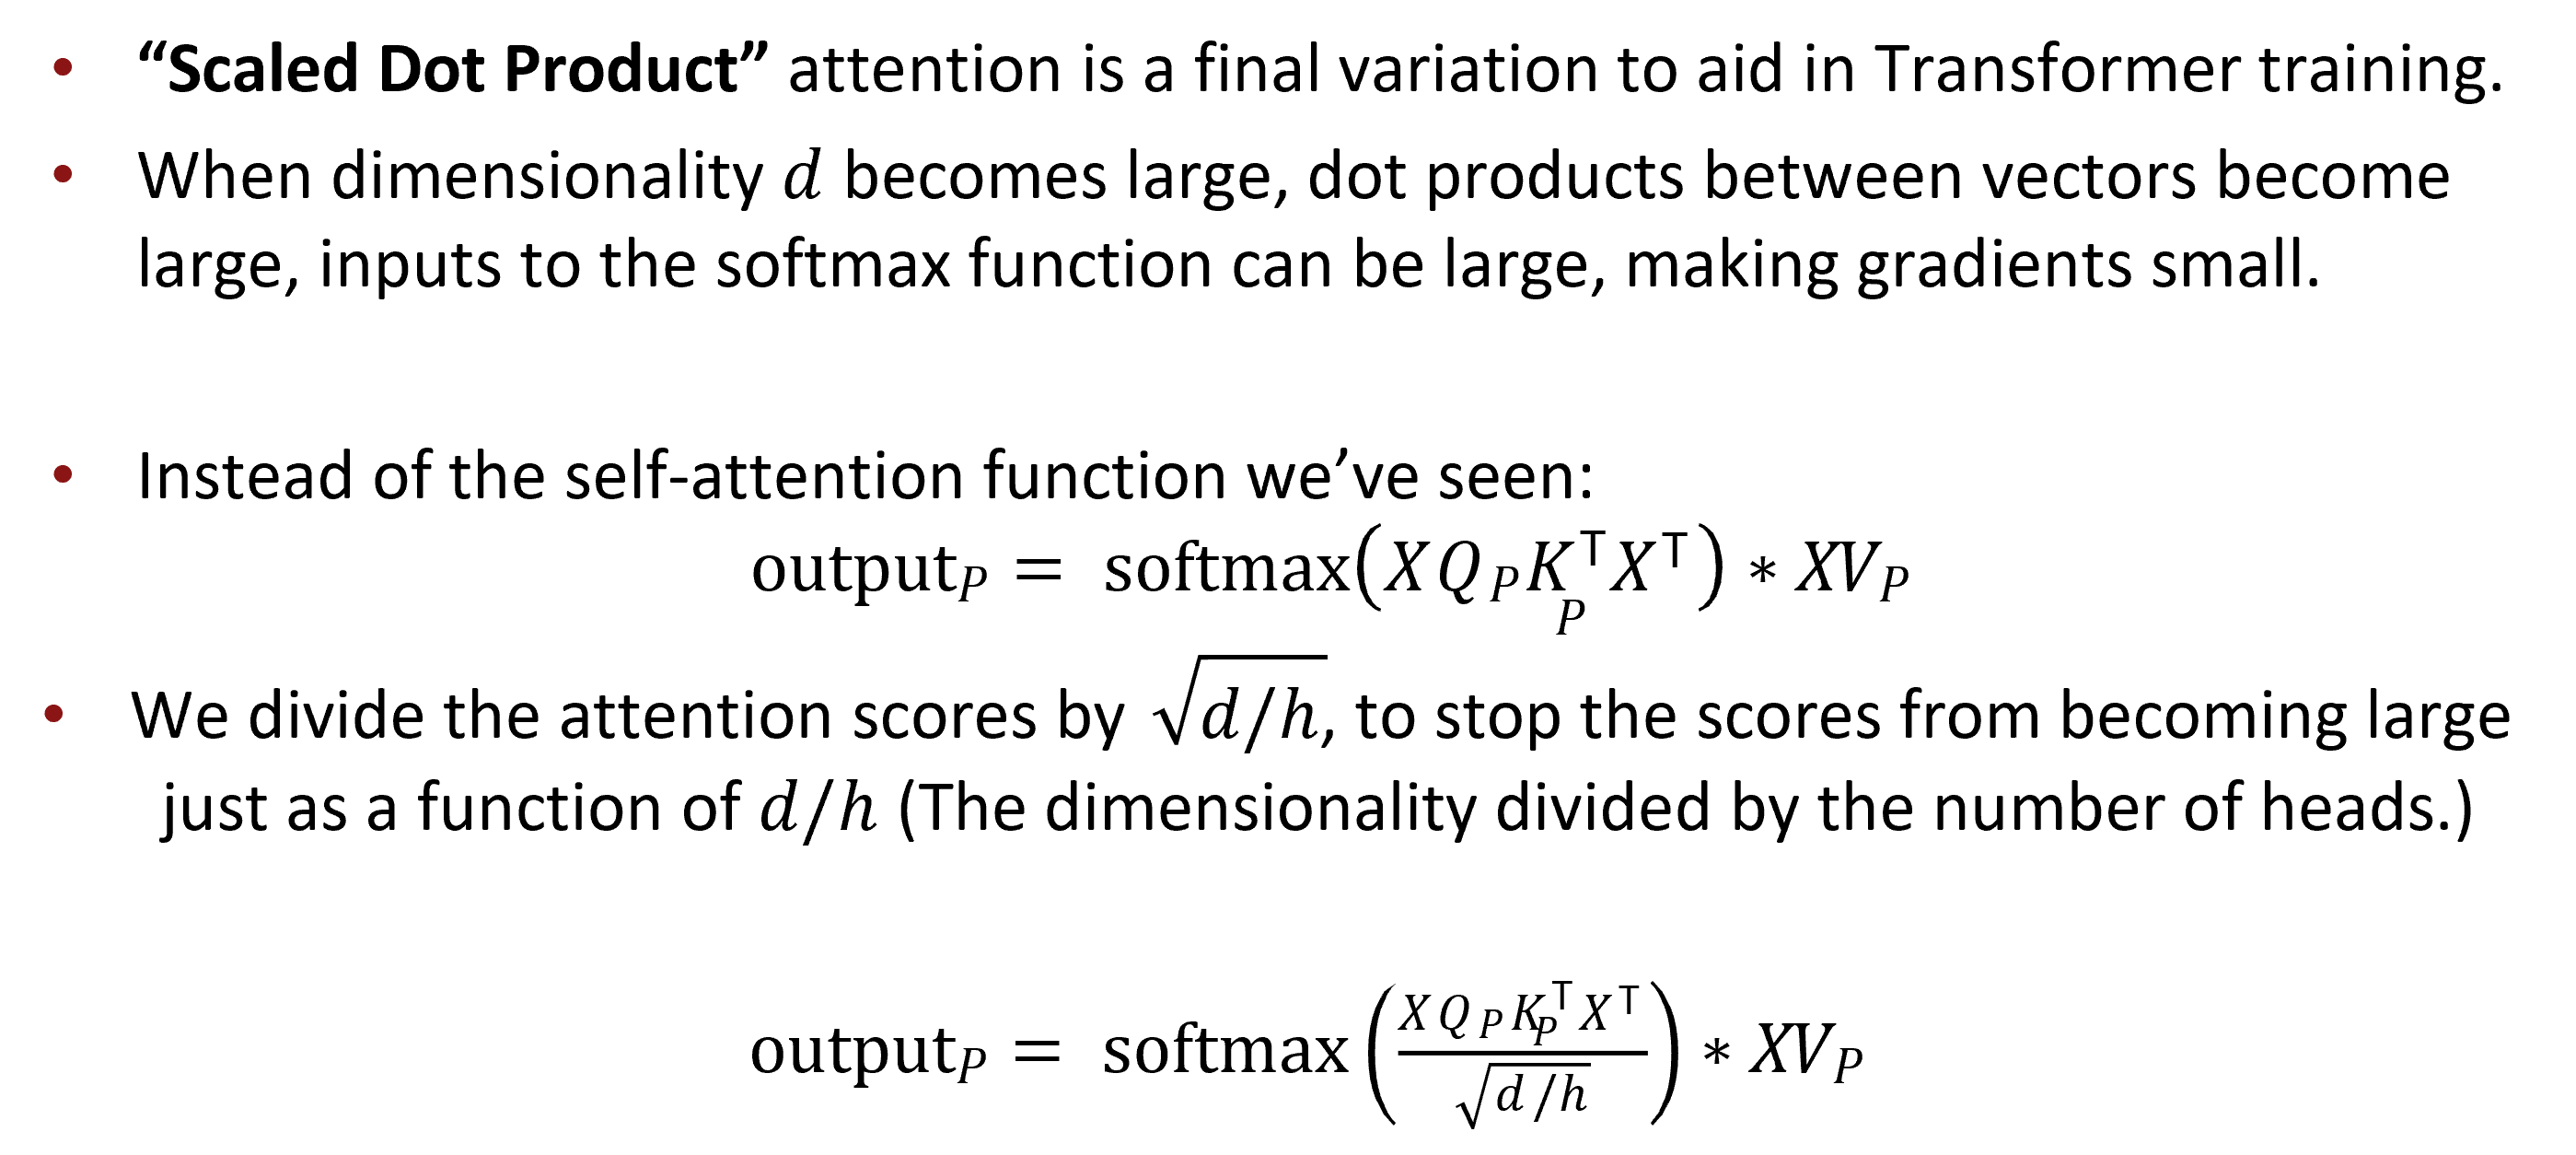
\includegraphics[width=\linewidth,keepaspectratio]{bert84}
			% \end{center}		
			
		
			% % {\tiny (Ref: John Hewitt)}

% \end{frame}

%%%%%%%%%%%%%%%%%%%%%%%%%%%%%%%%%%%%%%%%%%%%%%%%%%%%%%%%%%%%%%%%%%%%%%%%%%%%%%%%%%
\begin{frame}[fragile]\frametitle{}
\begin{center}
{\Large Encoder side is done}
\end{center}

\begin{itemize}
\item The encoder blocks then produce a final output, encoding. This vector is a rich, condensed representation of the most important information from the input.
\item So, ready with latent space, parallel word embedding of the input sentence ie BERT
\item The decoder uses self-attention and feed-forward layers, just like the encoder, however it has an additional component, the encoder-decoder attention layer. This layer allows the decoder to focus on significant places from the input sequence.
\end{itemize}

\end{frame}




%%%%%%%%%%%%%%%%%%%%%%%%%%%%%%%%%%%%%%%%%%%%%%%%%%%%%%%%%%%%%%%%%%%%%%%%%%%%%%%%%%
\begin{frame}[fragile]\frametitle{}
\begin{center}
{\Large Decoder Side}
\end{center}
\end{frame}

%%%%%%%%%%%%%%%%%%%%%%%%%%%%%%%%%%%%%%%%%%%%%%%%%%%%%%%%%%%
\begin{frame}[fragile]\frametitle{The Decoder Side - Overview}


\begin{center}
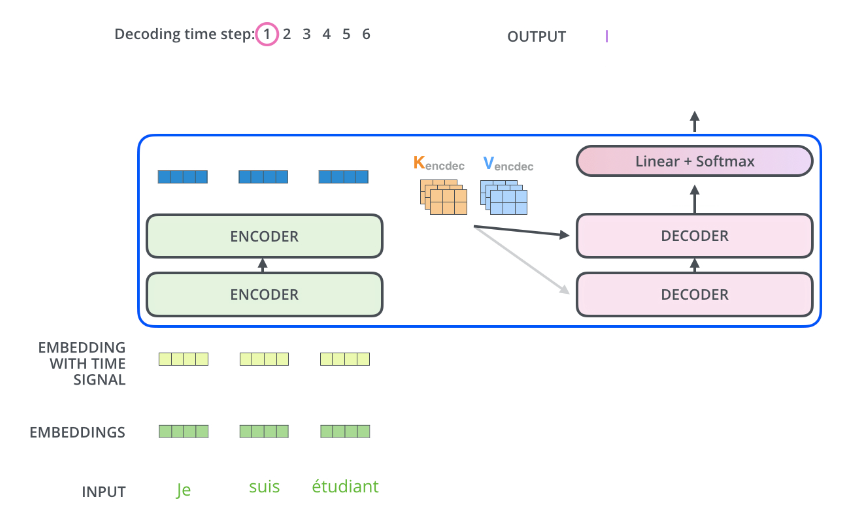
\includegraphics[width=0.8\linewidth,keepaspectratio]{transformer_decoding_1_jay}


{\tiny (Ref: ``The Illustrated Transformer'' - Jay Alammar)}
\end{center}	


The output of the top encoder is then transformed into a set of attention vectors K and V. These are to be used by each decoder in its ``encoder-decoder attention'' layer which helps the decoder focus on appropriate places in the input sequence.

\end{frame}

%%%%%%%%%%%%%%%%%%%%%%%%%%%%%%%%%%%%%%%%%%%%%%%%%%%%%%%%%%%
\begin{frame}[fragile]\frametitle{The Decoder Side - Overview}


\begin{center}
\includegraphics[width=0.8\linewidth,keepaspectratio]{transformer_decoding_2_jay}


{\tiny (Ref: ``The Illustrated Transformer'' - Jay Alammar)}
\end{center}	


The following steps repeat the process until a special symbol is reached indicating the transformer decoder has completed its output. The output of each step is fed to the bottom decoder in the next time step, and the decoders bubble up their decoding results just like the encoders did.
\end{frame}

%%%%%%%%%%%%%%%%%%%%%%%%%%%%%%%%%%%%%%%%%%%%%%%%%%%%%%%%%%%
\begin{frame}[fragile]\frametitle{The Decoder Side - Overview}



\begin{itemize}
  \item In the decoder, self-attention layers differ from those in the encoder.
    \begin{itemize}
      \item The self-attention layer in the decoder can only attend to earlier positions in the output sequence.
      \item This is achieved by masking future positions (setting them to $-\infty$) before the softmax step in the self-attention calculation.
    \end{itemize}
  \item The "Encoder-Decoder Attention" layer functions similarly to multiheaded self-attention.
    \begin{itemize}
      \item It generates its Queries matrix from the layer below it.
      \item The Keys and Values matrix are taken from the output of the encoder stack.
    \end{itemize}
\end{itemize}
\end{frame}

%%%%%%%%%%%%%%%%%%%%%%%%%%%%%%%%%%%%%%%%%%%%%%%%%%%%%%%%%%%%%%%%%%%%%%%%%%%%%%%%%%
\begin{frame}[fragile]\frametitle{}
\begin{center}
{\Large Output Embedding plus Positional Encoding}
\end{center}
\end{frame}

%%%%%%%%%%%%%%%%%%%%%%%%%%%%%%%%%%%%%%%%%%%%%%%%%%%%%%%%%%%%%%%%%%%%%%%%%%%%%%%%%%
\begin{frame}[fragile]\frametitle{}
\begin{center}
{\Large Masked Attention}
\end{center}
\end{frame}

%%%%%%%%%%%%%%%%%%%%%%%%%%%%%%%%%%%%%%%%%%%%%%%%%%%%%%%%%%%
\begin{frame}[fragile]\frametitle{Masked Attention Need}



\begin{itemize}
  \item  we need masking to make the training parallel. And the parallelization is good as it allows the model to train faster.
  \item  Example: to translate ``I love you'' to German
  \item The encoder works in parallel mode, takes the input sequence ("I love you")  and produces the numbers 11, 12, 13 as the vector representations of the input sequence.
  \item During the training we know that the translation should be ``Ich liebe dich'' with corresponding expected vector representations as 21, 22, 23.

\end{itemize}

{\tiny (Ref https://stackoverflow.com/questions/58127059/how-to-understand-masked-multi-head-attention-in-transformer)}

\end{frame}

%%%%%%%%%%%%%%%%%%%%%%%%%%%%%%%%%%%%%%%%%%%%%%%%%%%%%%%%%%%
\begin{frame}[fragile]\frametitle{Masked Attention Need}

As we actually know the expected outputs we can adjust the process and make it parallel. There's no need to wait for the previous step output.

\begin{itemize}
  \item  Parallel operation \#A. Inputs: 11, 12, 13. Trying to predict 21.
  \item Parallel operation \#B. Inputs: 11, 12, 13, and also 21. Trying to predict 22.
	\item Parallel operation \#C. Inputs: 11, 12, 13, and also 21, 22. Trying to predict 23.
\end{itemize}

All input-output pairs are ready.

{\tiny (Ref https://stackoverflow.com/questions/58127059/how-to-understand-masked-multi-head-attention-in-transformer)}

\end{frame}

%%%%%%%%%%%%%%%%%%%%%%%%%%%%%%%%%%%%%%%%%%%%%%%%%%%%%%%%%%%
\begin{frame}[fragile]\frametitle{Masked Attention Need}

Now we can clearly see why masking is done.

\begin{itemize}
  \item  Say for Parallel operation \#A. Inputs: 11, 12, 13. As it is trying to predict 21, it should not see any of 21, 22, 23, right? so all are masked.
  \item For Parallel operation \#B. Inputs: 11, 12, 13, and also 21. Trying to predict 22. Here we need 21, so thats unmasked, but 22, 23 are masked, as they to be predicted one by one. So here it hides  2nd and 3rd outputs.
	\item For Parallel operation \#C. Inputs: 11, 12, 13, and also 21, 22. Trying to predict 23. It hides 3rd output.
\end{itemize}

{\tiny (Ref https://stackoverflow.com/questions/58127059/how-to-understand-masked-multi-head-attention-in-transformer)}

\end{frame}

%%%%%%%%%%%%%%%%%%%%%%%%%%%%%%%%%%%%%%%%%%%%%%%%%%%%%%%%%%%
\begin{frame}[fragile]\frametitle{Masked Attention Need}


\begin{itemize}
  \item   implementation is inside of scaled dot-product attention by masking out (setting to $\infty$ ) all values in the input of the softmax which correspond to illegal connections.
  \item Note: during the inference (not training) the decoder works in the sequential (not parallel) mode as it doesn't know the output sequence initially. But it's different from RNN approach as Transformer inference still uses self-attention and looks at all previous outputs
\end{itemize}

{\tiny (Ref https://stackoverflow.com/questions/58127059/how-to-understand-masked-multi-head-attention-in-transformer)}

\end{frame}

%%%%%%%%%%%%%%%%%%%%%%%%%%%%%%%%%%%%%%%%%%%%%%%%%%%%%%%%%%%%%%%%%%%%%%%%%%%%%%%%%%
\begin{frame}[fragile]\frametitle{}
\begin{center}
{\Large Masked Multi-head Attention}
\end{center}
\end{frame}


%%%%%%%%%%%%%%%%%%%%%%%%%%%%%%%%%%%%%%%%%%%%%%%%%%%%%%%%%%%%%%%%%%%%%%%%%%%%%%%%%%
\begin{frame}[fragile]\frametitle{}
\begin{center}
{\Large Linear plus Softmax}
\end{center}
\end{frame}

%%%%%%%%%%%%%%%%%%%%%%%%%%%%%%%%%%%%%%%%%%%%%%%%%%%%%%%%%%%
\begin{frame}[fragile]\frametitle{The Final Linear and Softmax Layer}

\begin{itemize}
  \item The decoder stack produces a vector of floats as its output.
  \item How do we turn that into a word? That’s the job of the final Linear layer which is followed by a Softmax Layer.
  \item The Linear layer is a fully connected neural network projecting the decoder stack's output vector into a much larger vector known as a logits vector.
    \begin{itemize}
      \item Assuming a model vocabulary of 10,000 unique English words, the logits vector has 10,000 cells, each corresponding to the score of a unique word.
    \end{itemize}
  \item The softmax layer transforms these scores into probabilities, ensuring they are all positive and sum up to 1.0.
    \begin{itemize}
      \item The cell with the highest probability determines the chosen word, which serves as the output for the current time step.
    \end{itemize}
  \item Given a final vector from the neural network,
    \begin{itemize}
      \item This vector is expanded to a vocabulary-long vecto via $ m \times n$ neural network.
      \item Output is through a softmax function, causing the values to be compressed to the range of 0 to 1.
      \item Each value can be interpreted as a probability.
    \end{itemize}
  \item The index in the vocabulary vector with the highest probability determines the output word.
	
\end{itemize}
\end{frame}

%%%%%%%%%%%%%%%%%%%%%%%%%%%%%%%%%%%%%%%%%%%%%%%%%%%%%%%%%%%
\begin{frame}[fragile]\frametitle{The Final Linear and Softmax Layer}


\begin{center}
\includegraphics[width=\linewidth,keepaspectratio]{transformer_decoder_output_softmax_jay}


{\tiny (Ref: ``The Illustrated Transformer'' - Jay Alammar)}
\end{center}	

\end{frame}



% %%%%%%%%%%%%%%%%%%%%%%%%%%%%%%%%%%%%%%%%%%%%%%%%%%%%%%%%%%%
% \begin{frame}[fragile]\frametitle{Attending Encoder side}

% The Transformer Encoder: Scaled Dot Product [Vaswani et al., 2017]
			
			% \begin{center}
			% \includegraphics[width=\linewidth,keepaspectratio]{bert85}
			% \end{center}		
			
		
			% % {\tiny (Ref: John Hewitt)}

% \end{frame}

% %%%%%%%%%%%%%%%%%%%%%%%%%%%%%%%%%%%%%%%%%%%%%%%%%%%%%%%%%%%
% \begin{frame}[fragile]\frametitle{Attending Encoder side}

			% The Transformer Encoder: Scaled Dot Product [Vaswani et al., 2017]
			
			% \begin{center}
			% \includegraphics[width=\linewidth,keepaspectratio]{bert86}
			% \end{center}		
			
		
			% % {\tiny (Ref: John Hewitt)}

% \end{frame}

% %%%%%%%%%%%%%%%%%%%%%%%%%%%%%%%%%%%%%%%%%%%%%%%%%%%%%%%%%%%
% \begin{frame}[fragile]\frametitle{Attending Encoder side}

						% The Transformer Encoder: Scaled Dot Product [Vaswani et al., 2017]

			% \begin{center}
			% \includegraphics[width=\linewidth,keepaspectratio]{bert87}
			% \end{center}		
			
		
			% % {\tiny (Ref: John Hewitt)}

% \end{frame}

% %%%%%%%%%%%%%%%%%%%%%%%%%%%%%%%%%%%%%%%%%%%%%%%%%%%%%%%%%%%
% \begin{frame}[fragile]\frametitle{Attending Encoder side}

						% The Transformer Encoder: Scaled Dot Product [Vaswani et al., 2017]

			
			% \begin{center}
			% \includegraphics[width=\linewidth,keepaspectratio]{bert88}
			% \end{center}		
			
		
			% % {\tiny (Ref: John Hewitt)}

% \end{frame}

% %%%%%%%%%%%%%%%%%%%%%%%%%%%%%%%%%%%%%%%%%%%%%%%%%%%%%%%%%%%
% \begin{frame}[fragile]\frametitle{Cross-attention}

			% The Transformer Decoder: Cross-attention (details)
			
			% \begin{center}
			% \includegraphics[width=\linewidth,keepaspectratio]{bert89}
			% \end{center}		
			
		
			% % {\tiny (Ref: John Hewitt)}

% \end{frame}

% %%%%%%%%%%%%%%%%%%%%%%%%%%%%%%%%%%%%%%%%%%%%%%%%%%%%%%%%%%%
% \begin{frame}[fragile]\frametitle{Cross-attention}

			% The Transformer Decoder: Cross-attention (details)
			
			% \begin{center}
			% \includegraphics[width=\linewidth,keepaspectratio]{bert90}
			% \end{center}		
			
			% % {\tiny (Ref: John Hewitt)}

% \end{frame}

%%%%%%%%%%%%%%%%%%%%%%%%%%%%%%%%%%%%%%%%%%%%%%%%%%%%%%%%%%%%%%%%%%%%%%%%%%%%%%%%%%
\begin{frame}[fragile]\frametitle{}
\begin{center}
{\Large Backpropogation during training}
\end{center}
\end{frame}

%%%%%%%%%%%%%%%%%%%%%%%%%%%%%%%%%%%%%%%%%%%%%%%%%%%%%%%%%%%
\begin{frame}[fragile]\frametitle{Pre-training workflow}

% \begin{columns}
    % \begin{column}[T]{0.5\linewidth}
\begin{center}
\includegraphics[width=0.7\linewidth,keepaspectratio]{one-hot-vocabulary-example_jay}


{\tiny (Ref: ``The Illustrated Transformer'' - Jay Alammar)}
\end{center}		

		% \end{column}
    % \begin{column}[T]{0.5\linewidth}

\begin{itemize}
\item During training, an untrained model would go through the exact same forward pass. 
\item  But we have labeled dataset, ie inputs as well as output sentences. 
\item Say, vocab is of 6 words and using one hot encoding.
\item Assume our training sentences have only one pair, 'merci' and 'thanks'
\end{itemize}
    % \end{column}
  % \end{columns}	

\end{frame}

%%%%%%%%%%%%%%%%%%%%%%%%%%%%%%%%%%%%%%%%%%%%%%%%%%%%%%%%%%%
\begin{frame}[fragile]\frametitle{The Loss Function}

% \begin{columns}
    % \begin{column}[T]{0.5\linewidth}
\begin{center}
\includegraphics[width=0.6\linewidth,keepaspectratio]{transformer_logits_output_and_label_jay}


{\tiny (Ref: ``The Illustrated Transformer'' - Jay Alammar)}
\end{center}		

		% \end{column}
    % \begin{column}[T]{0.5\linewidth}

\begin{itemize}
\item Goal: For "merci", we want the output to be a probability distribution indicating the word ``thanks''. 
\item But since this model is not yet trained (meaning all weight matrices have random values), that’s unlikely to happen just yet.
\end{itemize}
    % \end{column}
  % \end{columns}	

\begin{itemize}
\item How do you compare two probability distributions? 
\item Say, we simply subtract one from the other. (For more details, look at cross-entropy and Kullback–Leibler divergence.)
\end{itemize}


\end{frame}

%%%%%%%%%%%%%%%%%%%%%%%%%%%%%%%%%%%%%%%%%%%%%%%%%%%%%%%%%%%
\begin{frame}[fragile]\frametitle{The Loss Function - More complex example}

For example – input: ``je suis etudiant'' and expected output: ``i am a student''. We want our model to successively output probability distributions where:

\begin{columns}
    \begin{column}[T]{0.5\linewidth}
\begin{center}
\includegraphics[width=\linewidth,keepaspectratio]{output_target_probability_distributions_jay}


{\tiny (Ref: ``The Illustrated Transformer'' - Jay Alammar)}
\end{center}		

		\end{column}
    \begin{column}[T]{0.5\linewidth}

\begin{itemize}
\item Each probability distribution is represented by a vector of width vocab\_size (6 in our toy example, but more realistically a number like 30,000 or 50,000)
\item The first probability distribution has the highest probability at the cell associated with the word ``i''
\item The second probability distribution has the highest probability at the cell associated with the word ``am''
\item And so on, until the fifth output distribution indicates ‘<EOS>’ symbol, which also has a cell associated with it from the 10,000 element vocabulary.
\end{itemize}
    \end{column}
  \end{columns}	

\end{frame}


%%%%%%%%%%%%%%%%%%%%%%%%%%%%%%%%%%%%%%%%%%%%%%%%%%%%%%%%%%%
\begin{frame}[fragile]\frametitle{The Loss Function - More complex example}

\begin{columns}
    \begin{column}[T]{0.5\linewidth}
\begin{center}
\includegraphics[width=\linewidth,keepaspectratio]{output_trained_model_probability_distributions_jay}


{\tiny (Ref: ``The Illustrated Transformer'' - Jay Alammar)}
\end{center}		

 We repeat this for positions \#2 and \#3…etc. This method is called ``beam search''
		\end{column}
    \begin{column}[T]{0.5\linewidth}

\begin{itemize}
\item Now, because the model produces the outputs one at a time, we can assume that the model is selecting the word with the highest probability from that probability distribution and throwing away the rest (greedy decoding)
\item Another way, take top 2, (say, ‘I’ and ‘a’ for example), then in the next step, run the model twice: once assuming the first output position was the word ‘I’, and another time assuming the first output position was the word ‘a’, and whichever version produced less error considering both positions \#1 and \#2 is kept.
\end{itemize}
    \end{column}
  \end{columns}	

\end{frame}

%%%%%%%%%%%%%%%%%%%%%%%%%%%%%%%%%%%%%%%%%%%%%%%%%%%%%%%%%%%
\begin{frame}[fragile]\frametitle{Pre-training workflow Summary}

\begin{columns}
     \begin{column}[T]{0.5\linewidth}
\begin{center}
\includegraphics[width=\linewidth,keepaspectratio]{transformer_training}


{\tiny (Ref: ``Transformers Explained Visually (Part 1): Overview of Functionality'' - Ketan Doshi)}
\end{center}		

		\end{column}
    \begin{column}[T]{0.5\linewidth}

\begin{itemize}
\item The input sequence is converted into Embeddings (with Position Encoding) and fed to the Encoder.
\item The stack of Encoders processes this and produces an encoded representation of the input sequence.
\item The target sequence is prepended with a start-of-sentence token, converted into Embeddings (with Position Encoding), and fed to the Decoder.
\end{itemize}
    \end{column}
  \end{columns}	

\end{frame}


%%%%%%%%%%%%%%%%%%%%%%%%%%%%%%%%%%%%%%%%%%%%%%%%%%%%%%%%%%%
\begin{frame}[fragile]\frametitle{Pre-training workflow Summary}

\begin{columns}
     \begin{column}[T]{0.5\linewidth}
\begin{center}
\includegraphics[width=\linewidth,keepaspectratio]{transformer_training}


{\tiny (Ref: ``Transformers Explained Visually (Part 1): Overview of Functionality'' - Ketan Doshi)}
\end{center}		

		\end{column}
    \begin{column}[T]{0.5\linewidth}

\begin{itemize}
\item The stack of Decoders processes this along with the Encoder stack’s encoded representation to produce an encoded representation of the target sequence.
\item The Output layer converts it into word probabilities and the final output sequence.
\item The Transformer’s Loss function compares this output sequence with the target sequence from the training data. This loss is used to generate gradients to train the Transformer during back-propagation
\end{itemize}
    \end{column}
  \end{columns}	

\end{frame}

%%%%%%%%%%%%%%%%%%%%%%%%%%%%%%%%%%%%%%%%%%%%%%%%%%%%%%%%%%%
\begin{frame}[fragile]\frametitle{Inference workflow Summary}

\begin{columns}
     \begin{column}[T]{0.5\linewidth}
\begin{center}
\includegraphics[width=\linewidth,keepaspectratio]{transformer_inference}


{\tiny (Ref: ``Transformers Explained Visually (Part 1): Overview of Functionality'' - Ketan Doshi)}
\end{center}		

		\end{column}
    \begin{column}[T]{0.5\linewidth}

\begin{itemize}
\item The input sequence is converted into Embeddings (with Position Encoding) and fed to the Encoder.
\item The stack of Encoders processes this and produces an encoded representation of the input sequence.
\item Instead of the target sequence, we use an empty sequence with only a start-of-sentence token. This is converted into Embeddings (with Position Encoding) and fed to the Decoder.
\item The stack of Decoders processes this along with the Encoder stack’s encoded representation to produce an encoded representation of the target sequence.
\end{itemize}
    \end{column}
  \end{columns}	

\end{frame}


%%%%%%%%%%%%%%%%%%%%%%%%%%%%%%%%%%%%%%%%%%%%%%%%%%%%%%%%%%%
\begin{frame}[fragile]\frametitle{Inference workflow Summary}

\begin{columns}
     \begin{column}[T]{0.5\linewidth}
\begin{center}
\includegraphics[width=\linewidth,keepaspectratio]{transformer_inference}


{\tiny (Ref: ``Transformers Explained Visually (Part 1): Overview of Functionality'' - Ketan Doshi)}
\end{center}		

Note that since the Encoder sequence does not change for each iteration, we do not have to repeat steps \#1 and \#2 each time.
		\end{column}
    \begin{column}[T]{0.5\linewidth}

\begin{itemize}
\item The Output layer converts it into word probabilities and produces an output sequence.
\item We take the last word of the output sequence as the predicted word. That word is now filled into the second position of our Decoder input sequence, which now contains a start-of-sentence token and the first word.
\item Go back to step \#3. As before, feed the new Decoder sequence into the model. Then take the second word of the output and append it to the Decoder sequence. Repeat this until it predicts an end-of-sentence token. 

\end{itemize}
    \end{column}
  \end{columns}	

\end{frame}


% %%%%%%%%%%%%%%%%%%%%%%%%%%%%%%%%%%%%%%%%%%%%%%%%%%%%%%%%%%%%%%%%%%%%%%%%%%%%%%%%%%
% \begin{frame}[fragile]\frametitle{}
% \begin{center}
% {\Large Decoder only Transformer}
% \end{center}
% \end{frame}

% %%%%%%%%%%%%%%%%%%%%%%%%%%%%%%%%%%%%%%%%%%%%%%%%%%%%%%%%%%%
% \begin{frame}[fragile]\frametitle{Steps}

% \begin{itemize}
% \item Input: Prompt + $<EOS>$ (added internally)
% \item Tokenize and covert all to vectors by same vectorizer, say word2vec
% \item Add positional embedding
% \item Masked self attention does similarity check with sentence, so far, with words added one at a time. So it looks at only past at that point in time. This is same Q K V calculation.
% \end{itemize}

% \begin{center}
% \includegraphics[width=0.6\linewidth,keepaspectratio]{masked_self_attention_1}

% {\tiny (Ref: Decoder-Only Transformers, ChatGPTs specific Transformer, Clearly Explained!!! - StatQuest with Josh Starmer)}
% \end{center}

% \end{frame}


% %%%%%%%%%%%%%%%%%%%%%%%%%%%%%%%%%%%%%%%%%%%%%%%%%%%%%%%%%%%
% \begin{frame}[fragile]\frametitle{Steps}

% Multi head masked self attention

% \begin{center}
% \includegraphics[width=\linewidth,keepaspectratio]{masked_self_attention_2}

% {\tiny (Ref: Decoder-Only Transformers, ChatGPTs specific Transformer, Clearly Explained!!! - StatQuest with Josh Starmer)}
% \end{center}

% \end{frame}


% %%%%%%%%%%%%%%%%%%%%%%%%%%%%%%%%%%%%%%%%%%%%%%%%%%%%%%%%%%%
% \begin{frame}[fragile]\frametitle{Steps}

% \begin{itemize}
% \item Add skip connection
% \item Take the first word encoded output, put it in Feed Forward fully connected layer.
% \item we already know the next word (within the prompt), that becomes output to be trained against.
% \end{itemize}

% \begin{center}
% \includegraphics[width=0.6\linewidth,keepaspectratio]{decoder_only_1}

% {\tiny (Ref: Decoder-Only Transformers, ChatGPTs specific Transformer, Clearly Explained!!! - StatQuest with Josh Starmer)}
% \end{center}

% \end{frame}